\documentclass[a4paper,12pt]{article}
 
%% Начало шапки
 
%% Настройка поддержки русского языка
\usepackage{cmap}                   % Поиск по кириллице
\usepackage{mathtext}               % Кириллица в формулах
\usepackage[T1,T2A]{fontenc}        % Кодировки шрифтов
\usepackage[utf8]{inputenc}         % Кодировка текста
\usepackage[english,russian]{babel} % Подключение поддержки языков
 
%% Настройка размеров полей
\usepackage[top=0.7in, bottom=0.75in, left=0.625in, right=0.625in]{geometry}
 
%% Математические пакеты
\usepackage{mathtools}              % Тот же amsmath, только с некоторыми поправками
\usepackage{amssymb}                % Математические символы
\usepackage{amsthm}                 % Оформление теорем
\usepackage{amstext}                % Текстовые вставки в формулы
\usepackage{amsfonts}               % Математические шрифты
\usepackage{icomma}                 % "Умная" запятая: $0,2$ --- число, $0, 2$ --- перечисление
\usepackage{enumitem}               % Для выравнивания itemize (\begin{itemize}[align=left])
\usepackage{array}                  % Таблицы и матрицы
\usepackage{multirow}
 
%% Алгоритмические пакеты и их настройки
\usepackage{algorithm}              % Шапка алгоритма
\usepackage{algorithmicx}           % Написание алгоритмов
\usepackage[noend]{algpseudocode}   % Написание псевдокода; убраны end
\usepackage{listings}               % Для кода на каком-либо языке программиования
\renewcommand{\algorithmicrequire}{\textbf{Ввод:}}              % Ввод
\renewcommand{\algorithmicensure}{\textbf{Вывод:}}              % Вывод
\floatname{algorithm}{Алгоритм}                                 % Название алгоритма
\renewcommand{\algorithmiccomment}[1]{\hspace*{\fill}\{// #1\}} % Комментарии
\newcommand{\algname}[1]{\textsc{#1}}                           % Вызов функции в алгоритме
 
%% Шрифты
\usepackage{euscript}               % Шрифт Евклид
\usepackage{mathrsfs}               % \mathscr{}
 
%% Графика
\usepackage[pdftex]{graphicx}       % Вставка картинок
\graphicspath{{images/}}            % Стандартный путь к картинкам
\usepackage{tikz}                   % Рисование всего
\usepackage{pgfplots}               % Графики
 
%% Прочие пакеты
\usepackage{indentfirst}                    % Красная строка в начале текста
\usepackage{epigraph}                       % Эпиграфы
\usepackage{fancybox,fancyhdr}              % Колонтитулы
\usepackage[colorlinks=true, urlcolor=blue]{hyperref}   % Ссылки
\usepackage{titlesec}                       % Изменение формата заголовков
\usepackage[normalem]{ulem}                 % Для зачёркиваний
\usepackage[makeroom]{cancel}               % И снова зачёркивание (на этот раз косое)
\usepackage{xcolor}
 
%% Прочее
\mathtoolsset{showonlyrefs=true}        % Показывать номера только у тех формул,
                                        % на которые есть \eqref{} в тексте.
\renewcommand{\headrulewidth}{1.8pt}    % Изменяем размер верхнего отступа колонтитула
\renewcommand{\footrulewidth}{0.0pt}    % Изменяем размер нижнего отступа колонтитула

%Прочее
\usepackage{forest} % Деревья

%% Определения
\newtheorem{definition}{Определение}
\newtheorem*{defin}{Определение}
\newcommand{\Pclass}{\mathsf{P}}
\newcommand{\NPclass}{\mathsf{NP}}
\newcommand{\coNPclass}{\mathsf{coNP}}
\newcommand{\NPCclass}{\mathsf{NPC}}
\newcommand{\Time}{\mathsf{TIME}}
\newcommand{\NTime}{\mathsf{NTIME}}
\newcommand{\ETime}{\mathsf{EXPTIME}}
\newcommand{\Class}{\mathsf{Class}}
\renewcommand{\P}{\mathcal{P}}
\newcommand{\E}{\mathsf{E}}

\newtheorem*{on1n}{Задача}
\newtheorem*{on1n1}{Задача №1}

\newtheorem{fulllemma}{Лемма}
\newtheorem*{sl1}{Следствие 1}
\newtheorem*{sl2}{Следствие 2}
\newtheorem*{scheme}{Утверждение 1}
\newtheorem{theorem}{Теорема}
\newtheorem*{proposal}{Предложение}
\newtheorem*{notice}{Замечание}
\newtheorem{statement}{Утверждение}
\newtheorem{consequence}{Следствие}
\newtheorem*{lemma}{Лемма}
\newtheorem*{kuk}{Теорема Кука-Левина}
\newtheorem*{timeteor}{Теорема об иерархии задач по времени}

\newcommand{\note}{\underline{Замечание:} }
\newcommand{\fact}{\underline{\textbf{Факт}:} }
\newcommand{\example}{\underline{Пример:} }
\newcommand{\sign}{\underline{Обозначения:} }
\newcommand{\statements}{\underline{Утверждения:} }

\newcommand{\Z}{\mathbb{Z}}
\newcommand{\N}{\mathbb{N}}
\newcommand{\Q}{\mathbb{Q}}
\newcommand{\R}{\mathbb{R}}
\renewcommand{\C}{\mathbb{C}}
\renewcommand{\L}{\mathscr{L}}
\newcommand{\A}{\mathcal{A}}
\newcommand{\B}{\mathcal{B}}
\newcommand{\Bb}{\mathcal{B}}
\newcommand{\Rr}{\mathcal{R}}
 
%% Информация об авторах
\title{\Huge{Алгоритмы и Структуры Данных \\ Мини-Кормен 2}}
\author{Вадим Гринберг\\по лекциям Сергея Александровича Объедкова}
\date{}

\begin{document}

\begin{titlepage}
  \begin{center}
  
  	{\HugeАлгоритмы и Структуры Данных}
	\\ \
	\\ \
	\\ \
	{\Huge \textbf{Мини-Кормен 2}}
    \\ \
    \\ \
    
    \begin{figure}[h]
    \begin{center}
        \begin{minipage}[h]{\linewidth}
        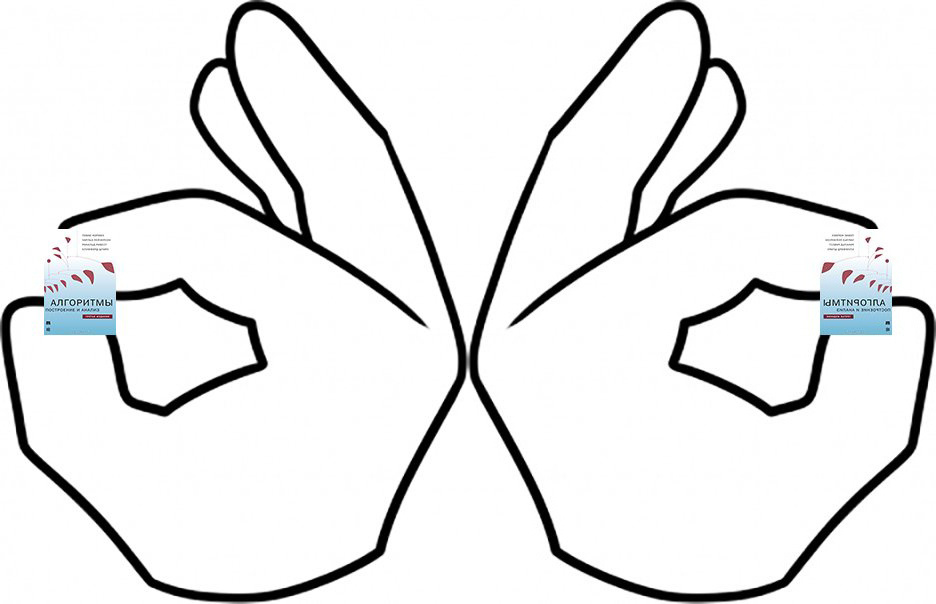
\includegraphics[height=18cm, width=\linewidth]{mini-kormen-2.jpg}
        \end{minipage}
    \end{center}
    \end{figure}
    \ \\
    
    {\Large Вадим Гринберг}\\\ \\
    {\large по лекциям Сергея Александровича Объедкова}
   
\end{center}
\end{titlepage}
 
\tableofcontents
\newpage
\section{Машины Тьюринга}

\subsection{Детерминированные МТ}

\begin{definition}
\textbf{Машина Тьюринга (МТ)} -- это кортеж из семи элементов:\\ $\langle Q,\ \Sigma,\ \Gamma,\ \delta,\ q_0,\ q_{accept},\ q_{reject}\rangle$, где 
\begin{itemize}
    \item $Q$ -- это множество состояний машины
    \item $\Sigma$ -- это алфавит
    \item $\Gamma$ -- это рабочий алфавит, в котором помимо алфавита $\Sigma$ есть также различные вспомогательные символы, такие как пробел $\textbf{\_}$, символ-разделитель $\#$ и другие.
    \item $\delta$ -- функция перехода: $\delta : Q \times \Gamma \to Q \times \Gamma \times \big\{\mathcal{L},\ \mathcal{R}\big\}$, которая сопоставляет паре из состояния и символа, на который сейчас смотрит головка МТ, тройку из нового состояния, символа, который головка записала на ленту, и направления, куда сдвинулась головка -- налево ($\mathcal{L}$), или направо ($\mathcal{R}$). 
    
    \example{$(q_{25},\ 'b') \to (q_7,\ 'a',\ \mathcal{L})$ -- изначально МТ была в состоянии 25, и головка смотрела на символ $b$. Затем МТ перешла в состояние 7, записала в ячейку символа $b$ на ленте символ $a$, и сдвинулась на ячейку влево.}
    \item $q_0$ -- начальное состояние МТ
    \item $q_{accept}$ -- допущение входной строки, состояние остановки
    \item $q_{reject}$ -- отвержение входной строки, состояние остановки
\end{itemize}
\end{definition}

Это было определение одноленточной МТ. Определение многоленточной Машины Тьюринга отличается функцией перехода $\delta$, которая для МТ с $k$ лентами примет следующий вид: $\delta : Q\times \Gamma^k \to Q \times \Gamma^k \times \big\{\mathcal{L},\ \mathcal{R}\big\}^k$, то есть, учитываются символы, на которые смотрит головка каждой из $k$ лент, и движения этих $k$ головок. 

\note{Можно также добавить символ движения $\mathcal{S}$, соответствующий случаю, когда головка не перемещается, а остаётся на месте, но обычно в этом нет необходимости.}

\note{$q_{accept} \neq q_{reject}$. При этом $q_0$ либо одно из данных состояний, либо не совпадает с ними.}

\begin{definition}
\textbf{Разрешаемый язык}, или \textbf{Множество допускаемых слов} $\mathscr{L}(M) = \{w \in \Sigma^*\ |\ \text{машина}\ M\ \text{допускает слово}\ w\}$. Иначе говоря, это множество слов, таких, что, получив на вход слово из данного множества, Машина Тьюринга $M$ в результате работы придёт в состояние $q_{accept}$.
\end{definition}

В частности, если $q_0 = q_{accept}$, то $\mathscr{L}(M) = \{\Sigma^*\}$, а если $q_0 = q_{reject}$, то $\mathscr{L}(M) = \varnothing$.

\begin{statement}
Одноленточные и многоленточные Машины Тьюринга эквивалентны в смысле полиномиальности времени работы.
\end{statement}
\begin{proof}
\ 
\begin{itemize}
    \item 1-МТ $\to$ $k$-МТ
    
        Заметим, что одноленточная МТ -- частный случай многоленточной, поэтому в эту сторону и доказывать нечего.
    \item $k$-МТ $\to$ 1-МТ
    
        Будем строить одноленточную Машину Тьюринга, эквивалентную имеющейся $k$-ленточной МТ. Предпримем следующие действия:
        \begin{enumerate}
            \item Добавим в рабочий язык $\Gamma$ символ-разделитель $\#$, которым мы разделим ленту по порядку на $k$ частей, каждая из которых будет соответствовать определённой строке $k$-ленточной МТ.
            \item Нужно при этом помнить, где находится (на какой смотрит символ) каждая из $k$ головок многоленточной МТ. Для этого на нашей одноленточной МТ в каждой из частей, соответствующих своим лентам в $k$-МТ, будем помечать символы (фактически добавляя в алфавит такой же символ, но "помеченный"), на которые смотрит головка МТ на соответственно каждой ленте.
            \item Начальное состояние МТ будет выглядеть так:\[\overset{\nabla}{c}w\underbrace{\#,\ \#, \ldots, \#}_{k - 1}\] где $c$ -- первый символ входного слова, $w$ -- оставшаяся его часть. Головка смотрит на $c$. Между разделителями ничего пока что нет (так как в $k$-МТ входное слово изначально появляется только в первой строке).
        \end{enumerate}
        
        Теперь проанализируем время имитации одноленточной МТ одного шага $k$-ленточной Машины Тьюринга. Посчитаем для начала время одного шага $k$-МТ. Ясно, что $T_k$ -- время одного шага $= O(\text{число всех занятых ячеек})$. Однако, на каждой ленте может находиться не более $t(n)$ символов, где $t$ -- какая-то полиномиальная функция, характеризующая время работы многоленточной МТ на каком-то входе размера $n$. Всего лент $k$, значит, на всех лентах суммарно не более $k \cdot t(n)$ занятых ячеек. Отсюда получаем, что размер ленты нашей одноленточной Машины Тьюринга составляет $O\big(t(n)\big)$. Тогда для того, чтобы сымитировать один шаг $k$-ленточной МТ, нам понадобится $O\big(t(n)^2\big)$ времени, что полиномиально зависит от времени одного шага на многоленточной МТ.
\end{itemize}

Итак, мы доказали, что одноленточные и многоленточные Машины Тьюринга эквивалентны в смысле полиномиальности времени работы.
\end{proof}

\subsection{Недетерминированные МТ}

\begin{definition}
\textbf{Недетерминированная Машина Тьюринга (НМТ)} -- та же обычная МТ, которая отличается только функцией перехода $\delta$:
\[\delta : Q \times \Gamma \to 2^{Q \times \Gamma \times \big\{\mathcal{L},\ \mathcal{R}\big\}}\] которая сопоставляет паре из состояния и символа, на который сейчас смотрит головка МТ, подмножество из троек типа (состояние, символ, движение).
\end{definition}
\example{$(q_{25},\ 'b') \to \begin{cases}(q_3,\ 'a',\ \mathcal{L}) \\ (q_4,\ 'c',\ \mathcal{R})\end{cases}$ -- выполняется лишь один из переходов.}

Машины Тьюринга можно представлять в виде деревьев выбора c ветвями. Тогда ДМТ выглядит так ($\bigcirc$ обозначает состояние):
\begin{center}
\begin{forest}
    for tree={
        if n children=0{
        font=\itshape,
        }{},
    }
    [$\bigcirc$ [$\bigcirc$[$\bigcirc$[$\bigcirc$]]]]
\end{forest}
\end{center}
А НМТ, соответственно, выглядит так:
\begin{center}
\begin{forest}
    for tree={
        if n children=0{
        font=\itshape,
        }{},
    }
    [$\bigcirc$ [$\bigcirc$ [$\bigcirc$] [$\bigcirc$]
                    [$\bigcirc$ [$\bigcirc$] [$\bigcirc$]]]
            [$\bigcirc$  [$\bigcirc$ [$\bigcirc$]]
                    [$\bigcirc$]]]]
\end{forest}
\end{center}

\begin{definition}
Говорят, что Машина Тьюринга \textbf{допускает} слово $w$, если в её дереве выбора, соответствующем данному входному слову, есть хотя бы один лист, отвечающий состоянию \(q_{accept}\).
\end{definition}
Можно провести аналог с ДКА и НКА. В частности, ДМТ допускает слово, если приходит в состояние $q_{accept}$, а НМТ допускает слово, если в $q_{accept}$ приходит хотя бы одна из её ветвей.

\note{\textbf{Временем работы} МТ является максимальная длина ветви дерева данной Машины Тьюринга.}
\newpage
\section{Основы теории вычислительной сложности. Основные классы}
\subsection{Абстрактные задачи. Кодирование.}
Ранее нами в курсе алгоритмов разбирались задачи, для которых есть алгоритм с полиномиальной сложностью. Это означает, что если размер входа равен \(n\), то сложность этого алгоритма равна \(O(n^k)\) для какой-то константы \(k\). Можно ли найти такой алгоритм для \emph{любой} задачи? К сожалению, нет. Стоит вспомнить знаменитую ``проблему останова'', которую невозможно решить на компьютере, сколько бы времени на неё не выделяли. Также есть примеры задач, для которых есть алгоритмы решения, но их сложность не является полиномиальной. Поэтому часто говорят, что полиномиальные задачи ``просты''.
    
Перед тем, как идти дальше, нужно понять~--- а как формально ввести понятие "задача"? Введём его так:
\begin{definition}
    \textbf{Задача} \(Q\)~--- это бинарное отношение на множестве \(I\) (множестве \textbf{экземпляров}) и множестве \(S\) (множестве \textbf{решений}).
\end{definition}
В теории вычислительной сложности в основном рассматривают \textbf{задачи разрешимости}, т.е. задачи, в которых \(S = \left\{0, 1\right\}\)~--- ``нет'' или же ``да''. 

Для того, чтобы компьютер решил задачу, нам необходимо передавать ему входные данные в понятном для него виде. Для этого используется \textbf{кодировка}~--- представление входных данных в виде слов над бинарным алфавитом. Вообще, всё может быть закодировано:
\begin{itemize}
    \item \textbf{Кодирование целого числа} -- полиномиально связано с его двоичным представлением.
    \item \textbf{Кодирование конечного множества} -- полиномиально связано с его кодированием в виде списка элементов.
    \item \textbf{Кодирование графа} -- полиномиально связано с количеством узлов в нём. Можно кодировать как в виде списка узлов и рёбер, так и в виде матрицы смежности.
\end{itemize}

\subsection{Класс \(\Pclass\)}
Будем полагать, что множество экземпляров~--- это \(\{0, 1\}^*\). Тогда язык, соответствующий задаче \(Q\) можно определить так:
\[L = \left\{x \in \{0, 1\}^* \mid Q(x) = 1\right\}\]
Теперь введём понятие \textbf{класса задач} \(\Pclass\) (Polynomial):
\begin{definition}
    \[\Pclass = \left\{\mathscr{L}(M) \mid M\text{~--- МТ с полиномиальным временем работы}\right\}\]
\end{definition}
Другими словами: задача лежит в классе \(\Pclass\) тогда и только тогда, когда для соответствующего ей языка можно построить допускающую детерминированную МТ с полиномиальным временем работы.
    
Теперь рассмотрим пару задач:
\begin{itemize}
    \item Задача о поиске пути между вершинами в графе. Очевидно, что она лежит в \(\Pclass\), так как входные данные представляют собой вершины и рёбра, а алгоритм решения (обход в ширину) полиномиален от количества вершин и рёбер.
    \item Задача проверки чисел на взаимную простоту: на вход подаются два числа \(x\) и \(y\), каждое из которых кодируется \(n\) символами. Взаимно просты ли они?
    Попробуем составить наивный алгоритм проверки:
    \begin{algorithm}[H]
        \caption{Наивная проверка чисел на взаимную простоту.}
        \begin{algorithmic}[1]
            \Statex
            \Require{Пара чисел \(x, y\)}
            \Ensure{Ответ на вопрос ``Верно ли, что \(x\) и \(y\) взаимно просты?''}
            \Statex
            \For{\(t = 1\) \textbf{to} min\((x, y)\)}
                \If{\(t \mid x\) \textbf{and} \(t \mid y\)}
                    \State \textbf{return} false
                \EndIf
            \EndFor
            \State \textbf{return} true
        \end{algorithmic}
    \end{algorithm}
    Как видно, он требует \(O(\text{min}(x, y))\) операций. Так как каждое число кодируется с помощью \(n\) нулей и единиц, то итоговая сложность составляет \(O(2^n)\). Не подходит.
        
    Значит ли это, что эта задача не имеет полиномиального решения? \emph{Нет.} Рассмотрим модификацию этого алгоритма, использующую алгоритм Евклида:
    \begin{algorithm}[H]
        \caption{Проверка чисел на взаимную простоту с использованием алгоритма Евклида.}
        \begin{algorithmic}[1]
            \Statex
            \Require{Пара чисел \(x, y\)}
            \Ensure{Ответ на вопрос ``Верно ли, что \(x\) и \(y\) взаимно просты?''}
            \Statex
            \State \(r \gets x \bmod y\)
            \While{\(r \neq 0\)}
                \State \(x \gets y\)
                \State \(y \gets r\)
                \State \(r \gets x \bmod y\)
            \EndWhile
            \State \textbf{return} \(y = 1\)
        \end{algorithmic}
    \end{algorithm}
    Теперь заметим следующее: за каждые две итерации цикла одно из чисел уменьшается по крайней мере вдвое. Для этого достаточно рассмотреть два случая~--- когда одно число меньше удвоенного второго или же больше его. Тогда алгоритм будет требовать \(O(\log(\text{min}(x, y))\) операций. Следовательно, сложность алгоритма составляет \(O(n)\) и эта задача принадлежит классу \(\Pclass\).
    \end{itemize}
    
Ранее мы говорили, что для того, чтобы компьютер решил задачу, входные данные нужно закодировать. Может ли кодировка повлиять на время работы алгоритма? Рассмотрим следующую задачу:

\textbf{Вход:} \(k \in \mathbb{Z}\)

\textbf{Время работы:} \(O(k)\)

Теперь рассмотрим, как будет зависить время работы от кодировки:
\begin{itemize}
\item \textbf{Унарная кодировка}: \(n = k \implies O(n)\)
\item \textbf{Бинарная кодировка}: \(n = \lfloor\log_2 k\rfloor + 1 \implies O(2^n)\)
\end{itemize}
Важно выбирать правильную кодировку. 

Стоит сказать, что, например, двоичная и десятичная кодировки полиномиально связаны (т.е. время работы алгоритма в одном и в другом случае будет отличаться с точностью до умножения на полином какой-то степени).

    \subsection{Классы \(\NPclass\) и \(\coNPclass\)}
    В теории вычислительной сложности также существует класс \(\NPclass\), который прославился с помощью гипотезы \(\Pclass = \NPclass\). Введём формальное определение:
    \begin{definition}
        \textbf{Класс} \(\NPclass\)~--- это класс задач таких, что они могут быть \textbf{верифицированы} за полиномиальное время.
    \end{definition}
    Что значит ``верифицировать'' задачу? Если язык \(\mathscr{L}\) лежит в классе \(\NPclass\), то существует функция от двух аргументов \(A(x, y)\)~--- \textbf{алгоритм верификации}~---  с полиномиальной сложностью от \(x\) такая, что \(x\) лежит в \(\mathscr{L}\) тогда и только тогда, когда для него существует \(y\) (его принято называть \textbf{сертификатом}) такой, что \(A(x, y) = 1\). При этом сертификат должен быть полиномиально зависим от размера \(x\).
    
    Достаточно логично, что \(\Pclass \subseteq \NPclass\), так как для задачи из класса \(\Pclass\) алгоритмом верификации служит сам алгоритм решения.
    
    Пример задачи из класса \(\NPclass\)~--- задача о распознании составных чисел.
    
    Возникает вопрос: а есть ли задача, которую нельзя верифицировать за полиномиальное время? \emph{Да.} Приведём пример, предварительно введя определение:
     \begin{definition}
        Неориентированный граф называется \textbf{Гамильтоновым}, если он содержит \textbf{Гамильтонов цикл} -- простой цикл, содержащий все вершины графа.
    \end{definition}
    \begin{algorithm}[H]
        \caption{Проверка графа на Гамильтоновость.}
        \begin{algorithmic}[3]
            \Require{граф \(G = (V, E)\)}
            \Ensure{Ответ на вопрос: ``Содержит ли граф \(G\) гамильтонов цикл?''}
            \State сформировать список перестановок вершин графа \(G\)
            \State проверить каждую перестановку
        \end{algorithmic}
    \end{algorithm}
    Проанализируем время работы. Пусть граф $G$ дан на вход в виде матрицы смежности размера $n$. Тогда $|V| = O(\sqrt{n})$, и время работы всего алгоритма проверки каждой перестановки составит $O(\sqrt{n!})$.
    
    Ещё один пример задачи, которая не факт, что входит в $\NPclass$ (на самом деле, она из $\coNPclass$, о котором будет сказано позднее):
    \begin{algorithmic}
        \Require{граф \(G\)}
        \Ensure{Ответ на вопрос: ``Правда ли, что граф \(G\) не гамильтонов?''}
    \end{algorithmic}
    В данном случае сертификат будет экспоненциален от размера входных данных, так как придётся проверить все циклы в графе, которых экспоненциальное от числа вершин количество.
    
    Ранее было введено определение недетерминированной машины Тьюринга. Теперь можно сформулировать другое определение класса \(\NPclass\) (Nondetermi\-nistic Polynomial, а не Not Polynomial, как может сначала показаться):
    \begin{definition}
        \textbf{Класс} \(\NPclass\)~--- это множество языков \(\mathscr{L}(M)\), где \(M\)~--- это недетерминированная машина Тьюринга с полиномиальным временем работы.
    \end{definition}
    Возникает разумный вопрос~--- а почему это определение равносильно предыдущему? Ясно, что по алгоритму верификации можно построить недетерминированную Машину Тьюринга (случайно выбираем сертификат и запускаем работу). Обратно: если имеется НМТ, то путь по ветвям, оканчивающийся $q_{accept}$, и является сертификатом.
    
    Также принято параллельно с классом \(\NPclass\) вводить класс \(\coNPclass\):
    \begin{definition}
        \[\coNPclass = \left\{\overline{\mathscr{L}} = \Sigma^* \setminus \mathscr{L} \mid \mathscr{L} \in \NPclass \right\}\]
    \end{definition}
    Иначе говоря, класс \(\coNPclass\) суть класс дополнений языков из \(\NPclass\).
    В качестве упражнения покажите, что \(\Pclass \subseteq \coNPclass\).
\newpage
\section{\(\NPclass\)-полные задачи}

\note{По поводу терминологии: вообще понятия "языка" и "задачи" в теории алгоритмов являются различными, но мы их используем почти как синонимы. Формально, задача -- это <<условие>> и <<ответ>> (\textbf{да} или \textbf{нет}). А язык -- это множество условий, на которые ответ \textbf{да}. Просто, когда мы говорим о языке, мы рассматриваем МТ, разрешающую (допускающую) данный язык, то есть, определяющую, лежит ли поданное на вход слово в рассматриваемом языке. В то же время, если говорить о задаче, то мы рассматриваем МТ, решающую данную задачу (на которую ответом будет \textbf{да} или \textbf{нет}, что аналогично допущению языка). Поэтому можно говорить о классах $\Pclass$ и $\NPclass$ как о классах языков, так и о классах задач.}

Введём пока что условное определение $\NPclass$-полных задач.

\begin{defin}[неформальное]
    \textbf{Класс} \(\NPCclass\)~--- это множество самых трудных задач, которые далеко не факт, что имеют решение за полиномиальное время.
\end{defin}
Один из самых важных вопросов современной науки об алгоритмах -- это вопрос "совпадают ли классы $\Pclass$ и $\NPclass$" ($\Pclass = \NPclass\ ??$). Причём оба возможных варианта ответа -- \textbf{да} или \textbf{нет}. Ответ неизвестен, однако понятие $\NPclass$-полноты, облегчает поиск ответа на данный вопрос, \textbf{каким бы ответ ни был}.
\begin{itemize}
    \item \textbf{ДА} -- тогда достаточно взять $\NPCclass$ задачу и придумать к ней полиномиальное решение.
    \item \textbf{НЕТ} -- привести пример такой $\NPclass$-полной задачи $\NPclass$, которая точно не лежит в $\Pclass$.
\end{itemize}
Проблема в том, что неизвестно, есть ли что-то помимо $\NPCclass$ и $\Pclass$, так как некоторые $\NPclass$ задачи на самом деле являются $\Pclass$. Более того, вполне может оказаться, что даже для $\NPCclass$ задачи существует полиномиальное решение. Отсюда разделение на подобные классы весьма условно.

Будем рассматривать некоторые задачи $\NPCclass$.
\begin{algorithm}[H]
    \caption{\textbf{Задача} $SAT$}
    \begin{algorithmic}
        \Require{Булева формула}
        \Ensure{Ответ на вопрос: ``выполнима ли булева формула??''}
    \end{algorithmic}
\end{algorithm}
\begin{definition}
    Булева формула называется \textbf{выполнимой}, если существует такое \textbf{означивание} -- упорядоченная комбинация значений переменных формулы -- что формула при данном означивании принимает значение 1 (Истина).
\end{definition}
Пример выполнимой булевой формулы: $x \vee y$. Пример невыполнимой булевой формулы: $x \wedge \neg x$. Одним из возможных решений задачи $SAT$ является полный перебор всех возможных означиваний, однако такое решение будет экспоненциально зависеть от числа переменных.

Несложно заметить, что $SAT \in \NPclass$, так как существует полиномиальный алгоритм верификации, сертификатом для которого будут просто значения переменных при означивании. Хороший вопрос, решается ли задача $SAT$ за полиномиальное время. Была сформулирована и доказана следующая теорема:
\begin{kuk}
\[SAT \in \Pclass \Longleftrightarrow \Pclass = \NPclass\]
\end{kuk}
В ней, по факту, подразумевается следующее: если для задачи $SAT$ существует решение за полиномиальное время, то для всех остальных языков (задач) класса $\NPclass$ также существует решение за полиномиальное время. Как это вообще возможно? Суть в том, что все эти языки $\textbf{сводятся}$ к задаче $SAT$ за полиномиальное время. Дадим строгое определение \textbf{сводимости}.
\begin{definition}
    Функция $f : \Sigma^* \to \Sigma^*$ называется \textbf{вычислимой за полиномиальное время}, если существует такая ДМТ с полиномиальным временем работы, которая, получая на вход слово $w \in \Sigma^*$, заканчивает работу с $f(w)$ на ленте.
\end{definition}
\begin{definition}
    Язык $A$ \textbf{сводится} к языку $B$ за полиномиальное время, если существует функция $f$, вычислимая за полиномиальное время, такая, что $w \in A \Longleftrightarrow f(w) \in B$.
    
    Обозначение: $A \leqslant_p B$.
\end{definition}
Докажем основное утверждение о сводимости:
\begin{statement}
    Пусть $A \leqslant_p B$ и $B \in \Pclass$ (существует полиномиальный алгоритм решения задачи). Тогда $A \in \Pclass$.
\end{statement}
\begin{proof}
 Достаточно построить алгоритм, показывающий, что для языка $A$ тоже существует полиномиальное решение. Пусть у нас имеются Машины Тьюринга $M_A$, допускающая язык $A$, и $M_B$, допускающая язык $B$. Поскольку $A \leqslant_p B$, то $\exists$ полиномиальная $f$, удовлетворяющая определению выше. Построим алгоритм вычисления $M_A$:
 \begin{algorithmic}
    \Require{слово $w$}
    \State вычислить $f(w)$
    \State \Return $M_B\big(f(w)\big)$
 \end{algorithmic}
 Поскольку сама функция $f$ является вычислимой за полиномиальное время, то вычисление $f(w)$ потратит полиномиальное время. Кроме того, поскольку $B \in \Pclass$, то вычисление $M_B\big(f(w)\big)$ также займёт полиномиальное время (от размера $f(w)$, но $f(w)$ также вычисляется за полином)! Отсюда $M_A(w)$ также допускает слово $w$ за полиномальное время, что по определению означает, что $A \in \Pclass$.
\end{proof}
Теперь можно ввести два важных определения:
\begin{definition}
    Язык $\mathscr{L}$ -- $\NPclass$-трудный, если для любого языка $\mathscr{L}' \in \NPclass$ выполнено, что $\mathscr{L}' \leqslant_p \mathscr{L}$. (Сам $\mathscr{L}$ не обязательно лежит в $\NPclass$).
\end{definition}
\begin{definition}
    Язык $\mathscr{L}$ -- $\NPclass$-полный, если $\mathscr{L} \in \NPclass$ и $\mathscr{L}$ -- $\NPclass$-трудный.
\end{definition}
\newpage
\section{Примеры полиномиальных сведений}

Рассмотрим следующую задачу, именуемую \textbf{Задачей о КНФ}, или же $3SAT$:
\begin{algorithm}[H]
    \caption{\textbf{Задача} $3SAT$}
    \begin{algorithmic}
        \Require{3-КНФ $\varphi$ -- конъюнкция дизъюнкций из 3-х элементов}
        \Ensure{Ответ на вопрос: ``выполнима ли $\varphi$??''}
    \end{algorithmic}
\end{algorithm}
Пример 3-КНФ: $(\neg x \vee y \vee \neg z) \wedge (x \vee \neg y \vee z)$. Она выполнима -- решением будет означивание из всех 0. В более же сложных случаях весьма непросто ответить на поставленный вопрос.

Однако, данную задачу можно свести к другой, именуемой $NOT-ALL-EQUAL-3SAT$ $(NAE-3SAT)$:
\begin{algorithm}[H]
    \caption{\textbf{Задача} $NAE-3SAT$}
    \begin{algorithmic}
        \Require{3-КНФ $\varphi$}
        \Ensure{Ответ на вопрос: ``существует ли такое выполняющее означивание, что ни в какой скобке значения всех 3-х литер не одинаковы??''}
    \end{algorithmic}
\end{algorithm}
Сведём задачу $3SAT$ к $NAE-3SAT$. Но делать это будем не сразу, а провернём сначала один приём: сведём задачу $3SAT$ к так называемой $NAE-4SAT$ -- задаче с теми же условиями, что и для $NAE-3SAT$, только с 4 литерами в скобках. Для этого возьмём функцию $f$, вычислимую за полиномиальное время, которая получает на вход 3-КНФ $\varphi$, и каждую скобку переписывает так:
\begin{enumerate}
    \item Пусть есть дизъюнкция $(l_1 \vee l_2 \vee l_3)$
    \item Заменим её на скобку вида $(l_1 \circ l_2 \circ l_3 \circ t)$, добавив переменную $t \notin \varphi$, одну и ту же для всех скобок. $\circ$ условно обозначает следующую операцию: \textit{выражение из элементов, связанных $\circ$, истинно тогда и только тогда, когда среди связанных литер не все литеры одинаковы}.
\end{enumerate}
Наша форма из примера выше приобретёт следующий вид: $(\neg x \circ y \circ \neg z\circ t)\wedge(x \circ \neg y \circ z \circ t)$.
\begin{statement}
    $3SAT \leqslant_p NAE-4SAT$
\end{statement}
\begin{proof}
    Докажем по определению, используя введённую ранее функцию $f$: $\varphi \in 3SAT \Longleftrightarrow f(\varphi) \in NAE-4SAT$. Иными словами, нужно показать, что $\varphi$ является выполнимой $3SAT$ формулой тогда и только тогда, когда $f(\varphi)$ является выполнимой $NAE-4SAT$ формулой.
    \begin{itemize}
        \item $\varphi \in 3SAT \Longrightarrow f(\varphi) \in NAE-4SAT$
        
        Пусть $\varphi \in 3SAT$. Тогда существует  такое означивание, что $\varphi$ истинно. Зафиксируем это выполняющее означивание. При данном означивании в каждой скобке $(l_1 \circ l_2 \circ l_3 \circ t)$ \underline{хотя бы одна} из литер $l_1,\ l_2,\ l_3$ истинна. По свойству $NAE$-КНФ, чтобы скобка была истинна, не все литеры должны быть одинаковы. Но тогда сделаем $t$ ложной (равной 0) -- таким образом мы добьёмся выполнения условий задачи $NAE-4SAT$. В итоге мы, применив функцию $f$ к $\varphi \in 3SAT$, получили $f(\varphi) \in NAE-4SAT$.
        \item $f(\varphi) \in NAE-4SAT \Longrightarrow  \varphi \in 3SAT$
        
        Пусть $f(\varphi)$ -- выполнимая $NAE-4SAT$ КНФ. Рассмотрим выполняющее означивание для данной формы, перебрав все возможные варианты переменной $t$:
        \begin{itemize}
            \item $t = 0$. В таком случае в каждой скобке $(l_1 \circ l_2 \circ l_3 \circ t)$ \underline{хотя бы одна} литера истинна (аналогично рассуждению выше). Но тогда, соотвественно, $(l_1 \vee l_2 \vee l_3) = 1$, и рассматриваемое означивание является выполняющим и для $\varphi$. 
            \item $t = 1$. В таком случае в каждой скобке $(l_1 \circ l_2 \circ l_3 \circ t)$ \underline{хотя бы одна} литера ложна (аналогично рассуждению выше). Но тогда можно просто инвертировать все литеры -- тогда $t$ станет равной 0, в каждой скобке хотя бы одна литера истинна, что приведёт нас к предыдущему случаю. Но тогда означивание, обратное рассматриваемому, будет выполняющим для $\varphi$.
        \end{itemize}
        В обоих случаях мы доказали существование выполняющего означивания для $\varphi \in 3SAT$. Отсюда напрямую следует, что $f(\varphi) \in NAE-4SAT \Longrightarrow  \varphi \in3SAT$.
    \end{itemize}
    Таким образом, наше утверждение доказано в обе стороны, и \\$3SAT \leqslant_p NAE-4SAT$.
\end{proof}

Теперь приступим к доказательству следующей сводимости:
\begin{statement}
    $NAE-4SAT \leqslant_p NAE-3SAT$
\end{statement}
\begin{proof}
    Зададим следующую функцию $f$: пусть у нас имеется скобка $(l_1 \circ l_2 \circ l_3 \circ l_4) = c_i$ -- один из конъюнктов ($i$-й) типа $NAE-4SAT$. Наша функция $f$ будет сопоставлять скобке $c_i$ конъюнкцию из пары скобок: $f(c_i) = (l_1 \circ l_2 \circ \xi_i) \wedge (l_3 \circ l_4 \circ \neg \xi_i)$, где $\xi_i$ -- новая переменная, уникальная для каждой скобки. Докажем по определению, используя данную функцию $f$, что $\varphi \in NAE-4SAT \Longleftrightarrow f(\varphi) \in NAE-3SAT$.
    \begin{itemize}
        \item $\varphi \in NAE-4SAT \Longrightarrow f(\varphi) \in NAE-3SAT$
        
        Пусть $\varphi \in NAE-4SAT$ выполнима. Тогда рассмотрим выполняющее означивание. В данном означивании некая скобка $c_i = (l_1 \circ l_2 \circ l_3 \circ l_4)$ принимает значение 1. По свойству $NAE-4SAT$, в скобке должна содержаться \underline{хотя бы одна} истина -- какая-то $l_k,\ k \in \{1,\ 2,\ 3,\ 4\}$, и \underline{хотя бы одна} ложь -- какая-то $l_r,\ r \in \{1,\ 2,\ 3,\ 4\}$, причём $k \neq r$. Переберём все возможные варианты $k$ и $r$:
        \begin{itemize}
            \item $[k,\ r] = [1,\ 2]$, что аналогично варианту $[k,\ r] = [3,\ 4]$. Рассмотрим первый. В данном случае в выражении $(l_1 \circ l_2 \circ \xi_i) \wedge (l_3 \circ l_4 \circ \neg \xi_i)$ первая скобка истинна вне зависимости от значения $\xi_i$. Тогда подбираем значениие $\xi_i$ таким, чтобы $l_3 \circ l_4 \circ \neg \xi_i = 1$ и выполнялись свойства $NAE-3SAT$ -- тогда выбранное означивание для $NAE-4SAT$ станет выполняющим и для $NAE-3SAT$.
            \item $k = [1,\ 2],\ r = [3,\ 4]$. В данном случае делаем $\xi_i$ ложным (равным 0). В таком случае в скобке $(l_1 \circ l_2 \circ \xi_i)$ есть как истина ($l_k$), так и ложь ($\xi_i$), и в скобке $(l_3 \circ l_4 \circ \neg \xi_i)$ есть как истина ($\neg \xi_i$), так и ложь ($l_r$). Тогда каждая из скобок будет принимать значение 1, отвечая свойствам $NAE-3SAT$, и выбранное означивание для $NAE-4SAT$ будет выполняющим и для $NAE-3SAT$.
        \end{itemize}
        Отсюда следует, что получившееся $f(\varphi) \in NAE-3SAT$, и, соотвественно, $\varphi \in NAE-4SAT \Longrightarrow f(\varphi) \in NAE-3SAT$.
        \item $f(\varphi) \in NAE-3SAT \Longrightarrow  \varphi \in NAE-4SAT$
        
        Пусть $f(\varphi)$ выполнима. Тогда рассмотрим выполняющее означивание. Пускай в полученной $f(\varphi)$ есть конъюнкция скобок $(l_1 \circ l_2 \circ \xi_i) \wedge (l_3 \circ l_4 \circ \neg \xi_i)$. 
        
        Предположим, что $l_1 = l_2 = l_3 = l_4 = 1$. Но тогда, чтобы удовлетворять свойствам $NAE-3SAT$, в скобке $(l_1 \circ l_2 \circ \xi_i)$ $\xi_i$ должно быть равно 0, и в то же время в скобке $(l_3 \circ l_4 \circ \neg \xi_i)$ $\neg \xi_i$ также должно быть равно 0, что невозможно. Аналогично для случая $l_1 = l_2 = l_3 = l_4 = 0$. Значит, случай, когда все литеры $l_1,\ l_2,\ l_3,\ l_4$ равны, получиться не мог, и хотя бы одна литера должны отличаться от остальных. Но это означает, что в исходной скобке $(l_1 \circ l_2 \circ l_3 \circ l_4)$ не все литеры равны между собой, и скобка удовлетворяет свойствам $NAE-4SAT$. Отсюда уже следует, что если полученная форма выполнима в смысле $NAE-3SAT$, то исходная форма также выполнима в смысле $NAE-4SAT$. А это, собственно, ровно то, что надо было доказать:  $f(\varphi) \in NAE-3SAT \Longrightarrow  \varphi \in NAE-4SAT$.
    \end{itemize}
    Таким образом, наше утверждение доказано в обе стороны, и $NAE-4SAT \leqslant_p NAE-3SAT$.
\end{proof}
Теперь можно легко доказать ранее высказанное утверждение:
\begin{statement}
    $3SAT \leqslant_p NAE-3SAT$
\end{statement}
\begin{proof}
    \[\begin{cases}3SAT \leqslant_p NAE-4SAT\\ NAE-4SAT \leqslant_p NAE-3SAT\end{cases} \Longrightarrow 3SAT \leqslant_p NAE-3SAT\]
\end{proof}

\newpage
\section{\(\NPCclass\)-языки}
Повторим определения, введёные на прошлой лекции:
\begin{definition}
    Язык $\mathscr{L}$ -- $\NPclass$-трудный, если $\forall\ \mathscr{L}' \in \NPclass: \mathscr{L}' \leqslant_p \mathscr{L}$. (Сам $\mathscr{L}$ не обязательно лежит в $\NPclass$).
\end{definition}
\begin{definition}
    Язык $\mathscr{L}$ -- $\NPclass$-полный, если:
    \begin{enumerate}
        \item $\mathscr{L} \in \NPclass$
        \item $\mathscr{L}$ -- $\NPclass$-трудный
    \end{enumerate}
    $\NPclass$-полные языки обозначаются как $\NPCclass$ (Nondeterme\-nistic Polynomial Complete).
\end{definition}
Докажем пару теорем.
\begin{theorem}
Пусть $\L \in \NPCclass$. Тогда, если $\L \in \Pclass$, то $\Pclass = \NPclass$.
\end{theorem}
\begin{proof}
    Пусть $\L' \in \NPclass$. Так как $\L \in \NPCclass$, то $\L' \leqslant_p \L$. Но, поскольку $\L \in \Pclass$, то $\L' \in \Pclass$, откуда $\Pclass = \NPclass$.
    
\end{proof}
\begin{theorem}
Если $B \in \NPCclass$ и $B \leqslant_p C \in \NPclass$, то $C \in \NPCclass$.
\end{theorem}
\begin{proof}
    Проверим оба условия, входящих в определение $\NPclass$-полного класса.
    \begin{enumerate}
        \item $C \in \NPclass$ -- по условию.
        \item Пусть $\L' \in \NPclass$. Так как $B \in \NPCclass$, то $\L' \leqslant_p B$, что по определению означает, что существует некая функция $f_{\L'B}$, вычислимая за полиномиальное время. Кроме того, $B \leqslant_p C$, что по определению означает, что существует некая функция $f_{BC}$, вычислимая за полиномиальное время.
        
        Но это означает, что $\L' \leqslant_p C$, так как существует функция $f_{\L'C}$, такая, что $f_{\L'C}(w) = f_{BC}\big(f_{\L'B}(w)\big)$ -- она также является вычислимой за полиномиальное время.
        
        Следовательно, $\forall\ \L' \in \NPclass: \L' \leqslant_p C$, откуда $C$ -- $\NPclass$-трудный по определению.
    \end{enumerate}
    Оба условия выполняются, значит, $C \in \NPCclass$.
\end{proof}
Посмотрим более пристально на задачу о выполнимости булевой формулы.
\textbf{Задача} $SAT$
\begin{algorithmic}
    \Require{Булева формула $\varphi(\vec{x})$, где $\vec{x}$ -- булев вектор $(x_1,\ x_2,\ \ldots,\ x_n)$}
    \Ensure{Ответ на вопрос: существует ли $\vec{x}$ такой, что $\varphi(\vec{x}) = 1$?}
\end{algorithmic}
Задачи различных классов можно трактовать несколько иначе, приведя эквивалентные определениям условия:
\begin{itemize}
    \item $A \in \NPclass\ ?? \Longleftrightarrow $ существует ли такой набор $\vec{y}$, что $P(\vec{y}) = 1$, где $P$ -- функция-описание (условие) задачи. По сути, $\vec{y}$ -- это сертификат. $P(y)$ должна работать за полиномиальное от размера описания (входа) время.
    \item $B \in \coNPclass\ ?? \Longleftrightarrow $ для любого ли набора $\vec{y}$ выполнено, что $Q(\vec{y}) = 1$, где $Q$ -- полиномиально проверяемое свойство. Мы перебираем все возможные $\vec{y}$. Если $B = \overline{A}$, то $Q = \neg P$. 
\end{itemize}


\newpage
\section{SAT и компания}
\subsection{Теорема Кука-Левина}
Ранее мы упоминали \textbf{Теорему Кука-Левина}. У неё существует альтернативная аналогичная формулировка, которую мы будем доказывать:
\begin{kuk}
\[SAT \in \NPCclass\]
\end{kuk}
\begin{proof}
    Сначала докажем следующую лемму:
    \begin{lemma}
    Пусть язык (задача) $\mathscr{A} \in \NPclass$. Тогда $\mathscr{A} \leqslant_p SAT$.
    \end{lemma}
    \begin{proof}
        Пусть $M$ -- НМТ со временем работы не больше $n^k - 3$ ($n$ -- длина входа, $k$ -- некое натуральное число), такая, что $\L(M) = \mathscr{A}$.
        
        Далее провернём следующий приём: пусть имеется какая-то конфигурация машины $M$: $acdb\overset{\nabla^{q_6}}{e}ac\textbf{\_}\textbf{\_}\ldots$ -- $M$ находится в состоянии $q_6$, головка смотрит на $e$. Преобразуем её к следующему виду:
        \[acdb\overset{\nabla^{q_6}}{e}ac\textbf{\_}\textbf{\_}\ldots \Longrightarrow \#acdbq_6eac\textbf{\_}\textbf{\_}\ldots\#\] -- записали всё в одну строку (состояние перед символом, на который указывает головка), и ограничили с обеих сторон символом-разделителем $\#$ (который не был в рабочем алфавите МТ изначально).
        
        Построим функцию $f$, необходимую для сводимости. 
        
        Рассмотрим одну ветвь НМТ и будем записывать получаемые конфигурации в специальную таблицу -- всего будет не более $n^k$ (время работы не более $n^k - 3$, и "влезет" ветвь любой длины), а столбцов, соответственно, не более $n^k - 3 + 3 = n^k$ (ко входному слову добавляются символ состояния и два символа разделителя $\#$).
        
        Пусть на вход $M$ было подано слово $w = w_1w_2w_3\ldots w_n$. Тогда таблица будет иметь следующий вид:
        \[ \bordermatrix{       
                & & & & & & & n^k & & & & & \cr
                & \# & q_0 & w_1 & w_2 &\ldots&w_n &\textbf{\_} &\textbf{\_} &\ldots&\ldots&\ldots &\textbf{\_} &\# \cr
                & \# & p_1 & q_1 & w_2 &\ldots&w_n &\textbf{\_} &\textbf{\_} &\ldots&\ldots&\ldots &\textbf{\_} &\# \cr
                &\dots &\dots &\dots &\dots &\dots &\dots &\dots &\dots &\dots &\dots&\dots&\dots &\dots \cr
            n^k &\dots &\dots &\dots &\dots &\dots &\dots &\dots &\dots &\dots&\dots&\dots         &\dots &\dots \cr
                &\#& p_1 & p_2 &\ldots&\ldots&\ldots& p_{m - 1} &q_{accept} &p_{m} &\textbf{\_} &\ldots &\textbf{\_} &\#  \cr
                &\dots &\dots &\dots &\dots &\dots &\dots &\dots &\dots&\dots&\dots&\dots &\dots &\dots \cr
                &\dots &\dots &\dots &\dots &\dots &\dots &\dots &\dots &\dots&\dots&\dots &\dots &\dots \cr}
        \]-- после окончания слова стоят пробельные символы \textbf{\_}.
        
        Функция $f$ будет сначала строить описание всех возможных ветвей МТ (по состояниям) в виде таблицы, со строками, заполненными по принципу выше.
        
        \fact{Слово $w$ находится в языке $\mathscr{A}$ тогда и только тогда, когда таблицу можно заполнить так, чтобы в какой-то из её ячеек появилось $q_{accept}$}
        
        Далее наша функция $f$ будет записывать факт выше в виде булевой формулы. То есть, выдаёт булеву формулу, описывающую все возможные ветви вычисления МТ $M$ на данном входном слове $w$. Это и позволит нам свести задачу к $SAT$.
        
        Пусть $Q$ -- множество состояний $M$, $\Gamma$ -- рабочий алфавит $M$. Множество $C = Q \cup \Gamma \cup \{\#\}$ -- символы, которыми мы заполняем таблицу.
        
        На входе МТ у нас всё то же слово $w$. Мы хотим получить такую булеву формулу $\varphi$, что $w \in \mathscr{A} \Longleftrightarrow \varphi \in SAT$. Наша $\varphi$ будет конъюнкцией 4-х формул:
        \[\varphi = \varphi_{cell} \wedge \varphi_{start} \wedge \varphi_{accept} \wedge \varphi_{move}\] где:
        \begin{itemize}
            \item $\varphi_{cell}$ -- условие, что в каждой ячейке таблицы ровно 1 элемент, причем этот элемент -- символ из рабочего алфавита
            \item $\varphi_{start}$ -- условие, что вход записан правильно
            \item $\varphi_{accept}$ -- условие, что в какой-то ячейке таблицы есть $q_{accept}$
            \item $\varphi_{move}$ -- условие, согласовывающее работу МТ
        \end{itemize}
        
        В нашей булевой формуле будут использоваться следующие переменные: $x_{ijs} = 1,\ i,\ j \in [1,\ n^k]$ означает, что в ячейке $(i,\ j)$ находится символ $s \in C$. Всего будет $O(n^{2k})$ переменных такого вида (по числу занятых ячеек таблицы).
        
        Теперь запишем все 4 формулы при помощи данных переменных:
        \[\varphi_{cell} = \bigwedge_{i,\ j \in [1,\ n^k]}\Biggl[\bigvee_{s \in C}x_{ijs} \wedge \bigwedge_{s \neq t \in C}(\neg x_{ijs} \vee \neg x_{ijt})  \Biggl]\] -- берём конъюнкцию по всем ячейкам на условие, что хотя бы 1 символ из $C$ да и есть в ячейке (большая дизъюнкция), но при этом в этой ячейке нет более никакого другого символа (а точнее, есть только этот), кроме данного (конъюнкция с большой конъюнкцией).
        \[\varphi_{start} = x_{11\#} \wedge x_{12q_0} \wedge x_{13w_1} \wedge \ldots \wedge x_{1(n+2)w_n} \wedge x_{1(n + 3)\_} \wedge \ldots \wedge x_{1(n^k - 1)\_} \wedge x_{1n^k\#}\] -- напрямую проверяем, что на вход подали именно то самое входное слово $w = w_1w_2w_3\ldots w_n$ и ни что иное.
        \[\varphi_{accept} = \bigvee_{i,\ j \in [1,\ n^k]}x_{ijq_{accept}}\] -- проверяем по всем ячейкам таблицы, что хотя бы в одной из них есть символ $q_{accept}$.
        
        Перед тем, как записывать в виде булевой формулы $\varphi_{move}$, введём понятие \textbf{допустимого окна}.
        \begin{definition}
            \textbf{Допустимым окном} -- \begin{tabular}{|c|*{3}{r|}|}
        \hline
        $a$ & $b$ & $c$ \\
        \hline
        $d$ & $e$ & $f$\\
        \hline
        \end{tabular}\\ -- будем называть прямоугольный срез таблицы ветви НМТ, такой, что каждая строка среза, начиная со второй, может быть получена за один такт работы данной Машины Тьюринга из предыдущей строки (в соответствии с правилами нашей МТ).
        \end{definition}
        Примеры допустимых и недопустимых окон :\\
        \begin{tabular}{|c|*{3}{r|}|}
        \hline
        $a $& $b$ & $q_1$ \\
        \hline
        $a$ & $q_2$ & $b$\\
        \hline
        $q_3$ & $a$ & $c$\\
        \hline
        \end{tabular} --допустимо,
        \begin{tabular}{|c|*{2}{r|}|}
        \hline
        $\#$ & $a$ \\
        \hline
        $\#$ & $a$\\
        \hline
        \end{tabular} -- допустимо,
        \begin{tabular}{|c|*{4}{r|}|}
        \hline
        $a$ & $b$ & $c$ & $q_3$ \\
        \hline
        $a$ & $q_3$ & $c$ & $d$\\ 
        \hline
        \end{tabular}--не допустимо,
        \ \\
        \ \\
        \begin{tabular}{|c|*{3}{r|}|}
        \hline
        $q_1$ & $a$& $a$ \\
        \hline
        $a$ & $q_2$ & $a$\\ 
        \hline
        \end{tabular} при отсутствии перехода $(q_1,\ a) \to$ -- не допустимо.
        
        Последний пример как раз иллюстрирует случай, когда в целом такое окно могло существовать, но по правилам перехода нашей МТ такой ситуации возникнуть не могло, и окно допустимым не является.
        
        С этого момента будем использовать допустимые окна размерами только $2\times 3$. Теперь будем описывать условия $\varphi_{move}$, используя допустимые окна. Пусть верхняя строка нашей таблицы -- это начальная конфигурация, и пусть каждое окно в нашей таблице допустимо -- иными словами, каждая строка таблицы, начиная со второй -- это конфигурация, легально следующая за конфигурацией предыдущей строки.
        
        Рассмотрим два случая, какие ячейки вообще могли получиться, и почему МТ будет работать корректно:
        \begin{enumerate}
            \item Ячейка не граничит с $q_i$ -- ячейкой с символом состояния -- и не содержит символы состояния. Тогда после одного такта Машины Тьюринга в ячейке всё останется без изменений -- соответственно в следующей строке таблицы содержимое данной ячейки ленты останется тем же, и МТ работает корректно.
            \item Ячейка граничит с $q_i$. Тогда рассмотрим \\окно $2\times 3$: \ \begin{tabular}{|c|*{3}{r|}|}
                        \hline
                         $a$& $q_i$ &$b$  \\
                        \hline
                         $c$& $d$ &$e$ \\ 
                        \hline
                        \end{tabular} -- на месте $a,\ b,\ c,\ d,\ e$ -- какие-то символы из $C$. Ячейка с состоянием в верхней строке посередине. По предположению, такое окно является допустимым. Но тогда и переход с первой строки на вторую будет легален, и Машина работает корректно.
        \end{enumerate}
        Теперь мы можем записать $\varphi_{move}$, используя терминологию допустимых окон:
        \begin{gather*}
        \varphi_{move} = \bigwedge_{\substack{1 \leqslant i < n^k \\ 1 < j < n ^ k}}\underset{j}{\begin{tabular}{|c|*{3}{r|}|}
                        \hline
                         &  & \\
                        \hline
                         &  & \\ 
                        \hline
                        \end{tabular}}\  i-\textbf{допустимые} \\
        \underset{j}{\begin{tabular}{|c|*{3}{r|}|}
                        \hline
                         &  & \\
                        \hline
                         &  & \\ 
                        \hline
                        \end{tabular}}\ i-\textbf{допустимые} = \bigvee_{\begin{tabular}{|c|*{3}{r|}|}
                        \hline
                         $a$& $b$ &$c$  \\
                        \hline
                         $d$& $e$ &$f$ \\ 
                        \hline
                        \end{tabular}-\text{допустимое окно}}\overset{\wedge}{x}\\
                \overset{\wedge}{x} = x_{i(j-1)a}\wedge x_{ijb} \wedge x_{i(j+1)c} \wedge x_{(i + 1)(j - 1)d} \wedge x_{(i + 1)je} \wedge x_{(i + 1)(j + 1)f} 
        \end{gather*}
    То есть, мы берём конъюнкцию по дизъюнкциям всех допустимых окон размера $2 \times 3$, у которых верхняя строка имеет номер $i$, а средний столбец -- номер $j$, таких, что эти окна являются допустимыми только при данных значениях этих 6 переменных в окне.
    
    Итак, мы закончили описание второго шага нашей функции $f$. Условие $w \in \mathscr{A} \Longleftrightarrow f(w) = \varphi \in SAT$ выполнено по построению. Осталось показать, что $f$ является вычислимой за полиномиальное время:
    \begin{itemize}
        \item $\varphi_{cell}$ -- так как $|C| = const$, то значит, пройдясь по всем ячейкам за $O(n^{2k})$, мы совершим на каждом шаге лишь константное число операций. Значит, время вычисления $\varphi_{cell}$ равно $O(n^{2k})$.
        \item $\varphi_{start}$ -- в первой строке у нас входное слово размера $n$, и ещё множество пробелов вплоть до конца строки. Тогда время проверки всей строки займёт $O(n^k)$, за которое и вычисляется $\varphi_{start}$.
        \item $\varphi_{accept}$ -- чтобы отыскать $q_{accept}$, нужно пробежаться по всем ячейкам таблицы, что потребует от $\varphi_{accept}$ времени $O(n^{2k})$.
        \item $\varphi_{move}$ -- мы идём по всем допустимым окнам, которые зависят от выбранных $(i,\ j)$, каждый не более $n^k$ -- это даёт минимум $O(n^{2k})$ действий. Далее, в каждом из окон мы ведём перебор содержимого -- для каждой из 6 ячеек мы проверяем $|C|$ значений, и всё это вместе. В итоге будет $|C|^6$ вариантов -- но это константная величина. Следовательно, ассимптотически это число ни на что не влияет. В итоге получаем время вычисления $O(n^{2k})$.
    \end{itemize}
    Как можно заметить, каждая из частей вычисляется за \underline{полиномиальное от $n$} время. Ну а так как\[\varphi = \varphi_{cell} \wedge \varphi_{start} \wedge \varphi_{accept} \wedge \varphi_{move}\] то для вычисления всего $\varphi$ мы просто последовательно будем вычислять каждую из 4 частей. Что, опять же, в итоге даст время вычисления $4 \cdot O(n^{2k}) = O(n^{2k})$ -- полиномиальное от $n$ -- размера входа.
    
    Таким образом, мы привели функцию $f$, вычислимую за полиномиальное время, такую, что $w \in \mathscr{A} \Longleftrightarrow f(w) = \varphi \in SAT$. А это по определению означает, что $\mathscr{A} \leqslant_p SAT$.
    
    Лемма таки доказана!
    \end{proof}
    Теперь проверим оба условия из определения $\NPclass$-полной задачи:
    \begin{enumerate}
        \item $SAT \in \NPclass$, так как сертификатом в алгоритме верификации будет любое выполняющее означивание (вычислимое за полиномиальное от входа время).
        \item Согласно лемме выше, $\forall\ \mathscr{A} \in \NPclass: \mathscr{A} \leqslant_p SAT$, что соответствует определению $\NPclass$-трудного языка.
    \end{enumerate}
    Оба условия выполняются, значит, $SAT \in \NPCclass$.
\end{proof}
\subsection{Сведения SAT}
Задачу $SAT$ можно свести к ещё более простым.

Для начала, представим $\varphi \in SAT$ в виде КНФ, то есть, чтобы вместо любых выполнимых булевых формул у нас были только КНФ. Рассмотрим для этого части $\varphi$ из предыдущей теоремы. $\varphi_{cell}$, $\varphi_{start}$,\ $\varphi_{accept}$ уже являются КНФ сами по себе. В $\varphi_{move}$ нужно просто раскрыть скобки в конъюнкции от дизъюнкций допустимых окон, и мы тоже придём к КНФ! Значит, задачу $\phi \in SAT$ можно представить в виде КНФ, не повлияв на время вычисления формулы (всего $O(n^{2k})$ скобок, на каждую потратим константное время).
\begin{statement}
    $SAT \leqslant_p 3SAT$
\end{statement}
\begin{proof}
    Докажем по определению, что существует такая вычислимая за полиномиальное время функция $f$, что $\varphi \in SAT \Longleftrightarrow f(\varphi) \in 3SAT$.
    
    Пусть $\varphi \in SAT$. Для начала представим её в виде КНФ, что не повлияет на ассимптотику. Достаточно просто предъявить алгоритм построения формулы из $3SAT$ по КНФ из $SAT$, сделав так, чтобы в скобках с дизъюнкциями было ровно 3 литеры.
    
    Приведём общий алгоритм для различного числа литер в дизъюнкции из $SAT$:
    \begin{enumerate}
        \item $(l_1) \Longrightarrow (l_1 \vee l_1 \vee l_1)$ -- повторяем 3 раза
        \item $(l_1 \vee l_2) \Longrightarrow (l_1 \vee l_1 \vee l_2)$ -- повторяем какую-то из двух литер ещё раз
        \item $(l_1 \vee l_2 \vee l_3) \Longrightarrow (l_1 \vee l_2 \vee l_3)$
        \item $(l_1 \vee l_2 \vee l_3 \vee l_4)$ -- введём дополнительную переменную $\xi$ --\\ $\Longrightarrow (l_1 \vee l_2 \vee \xi) \wedge (l_3 \vee l_4 \vee \neg \xi)$
        \item $(l_1 \vee l_2 \vee l_3 \vee l_4 \vee l_5)$ -- введём 2 дополнительных переменных $\xi_1$ и $\xi_2$ -- \\ $\Longrightarrow (l_1 \vee l_2 \vee \xi_1) \wedge (l_3 \vee \neg\xi_1 \vee \xi_2) \wedge (l_4 \vee l_5 \vee \neg\xi_2)$
        \item $(l_1 \vee l_2 \vee l_3 \vee l_4 \vee l_5 \vee l_6)$ -- аналогично случаю для 4 и 5 литер.
        \item И так далее...
    \end{enumerate}
    Корректность переходов для 1, 2 и 3 литер очевидна. Корректность перехода для 4 литер мы доказывали в предыдущем разделе. Корректность переходов для пяти и более литер доказывается аналогично случаю для 4 литер.
    
    Как мы видим, построение $f(\varphi) \in 3SAT$ по $\varphi \in SAT$ вида КНФ занимает полиномиальное от размера $\varphi$ время. В совокупности с тем, что перевод $\varphi$ в КНФ также занимает полиномиальное от размера $\varphi$ время, можно заключить, что функция $f$ является вычислимой за полиномиальное время.
    
    Таким образом, существует такая вычислимая за полиномиальное время функция $f$, что $\varphi \in SAT \Longleftrightarrow f(\varphi) \in 3SAT$. А это по определению означает, что $SAT \leqslant_p 3SAT$.
\end{proof}


\newpage
\section{\(\NPCclass\) задачи и SAT}
\subsection{Задача о сумме подмножества}
Рассмотрим теперь другую задачу, совершенно непохожую на $SAT$ на первый взгляд -- \textbf{Задача сумме подмножества}, или $Subset-Sum$.

\textbf{Subset-Sum}
\begin{algorithmic}
    \Require{числа $(x_1,\ \ldots,\ x_q)$, число $T\in \N$}
    \Ensure{Ответ на вопрос: ``существует ли подмножество индексов $S \subseteq \{1,\ \ldots,\ q\}$, такое, что $\sum\limits_{i \in S}x_i = T$ ??''}
\end{algorithmic}
\begin{theorem}
$Subset-Sum \in \NPCclass$
\end{theorem}
\begin{proof}
    Для начала докажем следующую лемму:
    \begin{lemma}
    $3SAT \leqslant_p Subset-Sum$
    \end{lemma}
    \begin{proof}
        Для начала, приведём такую функцию $f$, которая за полиномиальное время будет сводить задачу $3SAT$ к задаче о сумме подмножества, то есть:
        \[(l_1^1 \vee l_2^1 \vee l_3^1) \wedge \ldots \wedge (l_1^n \vee l_2^n \vee l_3^n) \overset{f}{\longrightarrow} (x_1,\ \ldots,\ x_q),\ T\]
        Пусть $y_i$ -- \underline{переменная} в $3SAT$. Сопоставим каждому $y_i$ две новых переменных: $a_i := y_i$ и $b_i := \neg y_i$. Иначе говоря, $\begin{cases}a_i\ \text{истинно} \Longleftrightarrow y_i\ \text{истинно} \\ b_i\ \text{истинно} \Longleftrightarrow y_i\ \text{ложно}\end{cases}$
        
        Мы хотим, чтобы в подмножестве $(x_1, \ldots, x_q)$ была от каждого $y_i$ выбрана ровно 1 переменная. Какими тогда должны быть $a_i,\ b_i,\ T$?
        
        Сделаем следующее. Пусть имеются переменные $y_1,\ \ldots,\ y_k$.
        Построим следующую таблицу, которая представляет собой соответствие между означиванием $3SAT$ и суммой.
        
        В ней будет сначала $k$ (по числу переменных) столбцов -- назовём их столбцами значений, потом ещё $n$ (по числу скобок) столбцов -- назовём их столбцами скобок. В строках мы будем последовательно записывать переменные $a_1,\ b_1,\ a_2,\ b_2,\ \ldots,\ a_k,\ b_k$, соотвествующие $y_1,\ \ldots,\ y_k$. Для каждого $a_i$ и $b_i$ в таблице в $i$-х столбцах значений будут записаны единицы (1). Для всех $j < i$ в стоблцах значений будут записаны 0, для всех $j > i$ в столбцах значений не будет записано ничего. В столбцах скобок мы для каждой переменной запишем символ $\ast$, такой, что: $\ast := \begin{cases}1,\ \text{если данная переменная есть в этой скобке}\\ 0,\ \text{если данной переменной нет в этой скобке}\end{cases}$
        
        Далее, запишем в строки по 2 переменные на каждую скобку: $c_{i1}$ и $c_{i2}$. В итоге получится $c_{11},\ c_{12},\ \ldots,\ c_{n1},\ c_{n2}$ -- $2n$ дополнительных переменных. В таблице для $c_{i1}$ и $c_{i2}$ мы для обеих в $i$-х столбцах скобок будут записаны единицы (1). Для всех $j > i$ в стоблцах скобок будут записаны 0, для всех $j < i$ в столбцах скобок не будет записано ничего. В столбцах значений у данных переменных пустота.
        
        В последней строке запишем число $T$. Во всех столбцах значений для $T$ пишем 1, во всех столбцах скобок для $T$ пишем 3.
        
        В общем виде таблица будет выглядеть так:
        \begin{gather*}
            \Downarrow\Downarrow\Downarrow\Downarrow\\
            \Downarrow\Downarrow\Downarrow\Downarrow\\
            \Downarrow\Downarrow\Downarrow\Downarrow\\
            \Downarrow\Downarrow\Downarrow\Downarrow\\
            \Downarrow\Downarrow\Downarrow\Downarrow\\
            \Downarrow\Downarrow\Downarrow\Downarrow
        \end{gather*}
        \begin{center}
        \begin{tabular}{||c||*{6}{r|}|*{5}{r|}|}
        \hline
        \hline
        Переменные\ $\downarrow\ \backslash$\ Разряды\ $\rightarrow$& $k$ & $k - 1$ & $\ldots$ & $3$ & $2$ & $1$ & 1 & 2 & $\ldots$ & $n - 1$ & $n$ \\
        \hline
        \hline
        $a_1$ & & &$\ldots$ & & &1 &$\ast$&$\ast$ &$\ldots$ & $\ast$ & $\ast$\\
        \hline
        $b_1$ & & &$\ldots$ & & &1 &$\ast$ &$\ast$ &$\ldots$ & $\ast$ & $\ast$ \\
        \hline
        $a_2$ & & &$\ldots$ & & 1&0 &$\ast$ &$\ast$ &$\ldots$ & $\ast$ & $\ast$\\
        \hline
        $b_2$ & & &$\ldots$ & & 1&0 &$\ast$ &$\ast$ &$\ldots$ & $\ast$& $\ast$ \\
        \hline
        $a_3$ & & &$\ldots$ &1 & 0&0 &$\ast$ &$\ast$ &$\ldots$ & $\ast$ & $\ast$\\
        \hline
        $b_3$ & & &$\ldots$ &1 &0 &0 &$\ast$ &$\ast$ &$\ldots$ & $\ast$ & $\ast$\\
        \hline 
        $\vdots$ & $\vdots$ &$\vdots$ &$\vdots$ &$\vdots$ &$\vdots$ &$\vdots$ &$\vdots$ &$\vdots$ &$\vdots$ &$\vdots$ &$\vdots$ \\
        \hline
        $a_{k - 1}$ & & 1&$\ldots$ & 0& 0&0 &$\ast$ &$\ast$ &$\ldots$ & $\ast$ & $\ast$\\
        \hline
        $b_{k - 1}$ & &1 &$\ldots$ & 0& 0&0 &$\ast$ &$\ast$ &$\ldots$ & $\ast$ & $\ast$\\
        \hline
        $a_k$ &1 & 0&$\ldots$ & 0& 0&0 &$\ast$ &$\ast$ &$\ldots$ & $\ast$ & $\ast$\\
        \hline
        $b_k$ &1 &0 &$\ldots$ & 0& 0&0 &$\ast$ &$\ast$ &$\ldots$ & $\ast$ & $\ast$\\
        \hline
        \hline
        $c_{11}$ & & &$\ldots$ & & & &1 &0 &$\ldots$ & 0 & 0\\
        \hline
        $c_{12}$ & & &$\ldots$ & & & &1 &0 &$\ldots$ & 0 & 0\\
        \hline
        $c_{21}$ & & &$\ldots$ & & & & &1 &$\ldots$ & 0 & 0\\
        \hline
        $c_{22}$ & & &$\ldots$ & & & & &1 &$\ldots$ & 0 & 0\\
        \hline 
        $\vdots$ & $\vdots$ &$\vdots$ &$\vdots$ &$\vdots$ &$\vdots$ &$\vdots$ &$\vdots$ &$\vdots$ &$\vdots$ &$\vdots$ &$\vdots$ \\
        \hline
        $c_{(n - 1)1}$ & & &$\ldots$ & & & & &&$\ldots$& 1 & 0\\
        \hline
        $c_{(n - 1)2}$ & & &$\ldots$ & & & & & &$\ldots$& 1 & 0\\
        \hline
        $c_{n1}$ & & &$\ldots$ & & & & &&$\ldots$&  & 1\\
        \hline
        $c_{n2}$ & & &$\ldots$ & & & & & &$\ldots$&  & 1\\
        \hline
        \hline
        $T$ &1 & 1&$\ldots$ & 1& 1&1 &3 &3 &$\ldots$ & 3 & 3\\
        \hline
        \hline
        \end{tabular}
        \end{center}
        В частности, для булевой формулы \[(y_1\vee \neg y_2 \vee \neg y_3) \wedge (\neg y_1 \vee \neg y_2 \vee y_3)\] таблица получится следующей:
        \begin{center}
        \begin{tabular}{||c||*{3}{r|}|*{2}{r|}|}
        \hline
        \hline
        Переменные\ $\downarrow\ \backslash$\ Разряды\ $\rightarrow$& $3$ & $2$ & $1$ & 1 & 2 \\
        \hline
        \hline
        $a_1$ & & & 1& 1& 0\\
        \hline
        $b_1$ & & & 1& 0&1 \\
        \hline
        $a_2$ & & 1& 0& 0&0 \\
        \hline
        $b_2$ & & 1& 0& 1& 1\\
        \hline
        $a_3$ & 1& 0& 0& 0&1 \\
        \hline
        $b_3$ & 1& 0& 0& 1& 0\\
        \hline
        \hline 
        $c_{11}$ & & & & 1& 0\\
        \hline
        $c_{12}$ & & & & 1& 0\\
        \hline
        $c_{21}$ & & & & & 1\\
        \hline
        $c_{22}$ & & & & & 1\\
        \hline
        \hline
        $T$ & 1& 1& 1& 3& 3\\
        \hline
        \hline
        \end{tabular}\end{center}
        
        Теперь объясним, а во имя чего, собственно, строить такую таблицу. Суть в том, что числа по строкам, что получились из $a_i$, $b_i$ и $c_{j1}$ с $c_{j2}$ -- это и есть наши числа $(x_1,\ \ldots,\ x_q)$, а получившееся число $T$ внизу таблицы -- это и есть то самое $T$, для которого необходимо найти суммирующее подмножество. Нам необходимо выбрать для каждой переменной $y_i$ одно из чисел $a_i$ или $b_j$ и только одно. Их мы будем складывать. Так как для $y_i$ у $a_i$ и $b_i$ единица стоит только в $i$-м столбце значений, то следовательно, при сложении мы в числе $T$ получим в начале ровно $k$ единиц. В $3SAT$ в каждой скобке по 3 литеры. Это значит, что в каждом из последних $n$ разрядов у числа $T$ будет стоять либо цифра 1 (как минимум, ведь булева формула должна быть выполнимой, раз она из языка $3SAT$), либо 2, либо 3 (максимум, так как в каждой скобке по 3 литеры) -- в зависимости от того, в каких скобках есть $a_i$ или $b_j$. Мы хотим, чтобы в последних $n$ разрядах в каждом суммарно вышло по 3. Для этого и заводятся $c_{ij}$, чтобы для каждой скобки докинуть от 0 до 2 дополнительных переменных, увеличив тем самым сумму в разряде до 3.
        
        В итоге мы получаем числа $a_i = 10^{i - 1} \cdot 10^n + d_{ai}$, $b_i = 10^{i - 1} \cdot 10^n + d_{bi}$, где числа $d_{ai}$ и $d_{bi}$ представляют из себя как раз те части из $\ast$. Ещё мы имеем числа $c_{j1}$ и $c_{j2}$, каждое из которых равно $10^{n - j}$. Также есть число $T$, которое в первых $k$ разрядах имеет 1, в последних $n$ разрядах имеет 3. Тогда:
        \begin{gather*}
            \{x_1,\ x_2,\ \ldots,\ x_q\} = \big\{a_1,\ \ldots a_k,\ b_1,\ \ldots,\ b_k,\ c_{11},\ c_{12},\ \ldots,\ c_{n1},\ c_{n2}\big\}\\
            T = \underbrace{11\ldots11}_{k}\underbrace{33\ldots33}_{n}
        \end{gather*}
        Тем самым мы свели задачу к $Subset-Sum$. Размер таблицы получился $(2n + 2k + 1)\times (n + k)$ -- полиномиальный от размера булевой формулы на входе функции $f$.
        
        Покажем теперь, что сведение корректно, то есть, $\varphi \in 3SAT \Longleftrightarrow f(\varphi) \in Subset-Sum$:
        \begin{itemize}
            \item $\varphi \in 3SAT \Longrightarrow f(\varphi) \in Subset-Sum$
            
            Пусть $\varphi \in 3SAT$ выполнима. Тогда существует выполняющее означивание. Рассмотрим его. Для каждой пары литер $y$ и $\neg y$ только одна из них истинна. Тогда, если $y_i = 1$, то выбираем к сумме $a_i$, если $y_i = 0$, то выбираем к сумме $b_i$. После этого в старших разрядах суммы (числа $T$ мы как раз получим $k$ единиц).
            
            Так как означивание выполняющее, то в каждой скобке 1, 2 или 3 литеры истинны. Тогда в последних разрядах $T$ получим 1, 2 или 3. Если получили 3, то не добираем $c_{j1}$ или $c_{j2}$. Если 2 -- докидываем к набору, образующему сумму, одно из $c_{j1}$ и $c_{j2}$. Если 1, то добавляем оба. Таким образом в сумме мы получили 3 в разряде.
            
            Это означает, что существует такое подмножество (которое мы набрали) чисел $a_i$, $b_i$ и $c_{j1}$ с $c_{j2}$, что в сумме дают $T = \underbrace{11\ldots11}_{k}\underbrace{33\ldots33}_{n}$, и задача лежит в  $Subset-Sum$.
            \item $f(\varphi) \in Subset-Sum \Longrightarrow \varphi \in 3SAT$
            
            Пусть в таблице, что мы получили, у нас существует подмножество чисел $a_i$, $b_i$ и $c_{j1}$ с $c_{j2}$, что в сумме дают число $T$ из таблицы же. Заметим, что в каждом столбце скобок находится ровно 5 единиц -- так как в скобках у нас было по 3 литеры, к каждой скобке ещё по единичке от $c_{j1}$ и $c_{j2}$. Это означает, что в итоговой сумме нет переносов разряда, и сумма корректна -- если написано 3, то суммируем 3 числа, если написано 1, то только одно число. Рассмотрим теперь $a_i$ и $b_i$. Если в наборе есть $a_i$, то значит, $y_i = 1$. Если в наборе есть $b_i$, то значит, $y_i = 0$. Следовательно, получаем некое означивание переменных $y_1,\ \ldots,\ y_k$.
            
            Покажем, что оно является выполняющим. Пусть $(l_1^j \vee l_2^j \vee l_3^j)$ -- $j$-я скобка. В $j$-м столбце скобок в строке числа $T$ стоит 3 -- значит, было выбрано 3 числа. Так как из чисел $c_{j1}$ и $c_{j2}$ мы могли выбрать максимум 2, то следовательно, было выбрано хотя бы одно число  из множеств $a_i$ и $b_i$, которе имеет 1 в $j$-м столбце скобок, и хотя бы одна из литер $l_1^j,\ l_2^j,\ l_3^j$ истинна. Но тогда и вся дизъюнкция истинна. Так для каждой скобки. В итоге получаем, что действительно существует выполняющее означивание, по которому строится набоо суммирования числа $T$.
        \end{itemize}
        Таким образом, мы привели функцию $f$, вычислимую за полиномиальное время, такую, что $\varphi \in 3SAT \Longleftrightarrow f(\varphi) \in Subset-Sum$. А это по определению означает,\\ что $3SAT \leqslant_p Subset-Sum$.
    \end{proof}
    Теперь проверим оба условия из определения $\NPclass$-полной задачи:
    \begin{enumerate}
        \item $Subset-Sum \in \NPclass$, так как сертификатом в алгоритме верификации будет просто набор индексов, таких, что соответствующие числа образуют в сумме $T$. Суммировать числа и сравнивать мы можем за полиномиальное время.
        \item Согласно лемме выше, $3SAT \leqslant_p Subset-Sum$, а так как $3SAT \in \NPCclass$, то значит, $\forall\ \mathscr{A} \in \NPclass: \mathscr{A} \leqslant_p 3SAT \leqslant_p Subset-Sum$, что соответствует определению $\NPclass$-трудного языка.
    \end{enumerate}
    Оба условия выполняются, значит, $Subset-Sum \in \NPCclass$.
\end{proof}

\subsection{Задача о рюкзаке}
Вспомним задачу о рюкзаке:

\textbf{Knapsack}
\begin{algorithmic}
    \Require{числа $(w_1,\ \ldots,\ w_q)$ -- веса предметов\\ числа $(v_1,\ \ldots,\ v_q)$ -- стоимости предметов \\ $W$ -- максимальный вес рюкзака}
    \Ensure{Набор предметов как можно большей суммарной стоимости при данных ограничениях на вес}
\end{algorithmic}
Переформулируем задачу следующим образом:
\begin{algorithmic}
    \Require{числа $(w_1,\ \ldots,\ w_q)$ -- веса предметов\\ числа $(v_1,\ \ldots,\ v_q)$ -- стоимости предметов \\ $W$ -- максимальный вес рюкзака \\ $V$ -- стоимость}
    \Ensure{Ответ на вопрос: ``Существует ли подмножество индексов\\ $S \subseteq \{1,\ \ldots,\ q\}$, такое, что $\sum\limits_{i \in S}w_i \leqslant W$ и $\sum\limits_{i \in S}v_i \geqslant V$ ??''}
\end{algorithmic}
Будем теперь рассматривать задачу о рюкзаке в данной формулировке.
\begin{theorem}
$Knapsack \in \NPCclass$.
\end{theorem}
\begin{proof}
    Для начала докажем следующую лемму:
    \begin{lemma}
    $Subset-Sum \leqslant_p Knapsack$
    \end{lemma}
    \begin{proof}
        Приведём функцию $f$, преобразующую задачу о сумме подмножества к задаче о рюкзаке напрямую за полиномиальное время.
        
        Пусть имеется множество чисел $\{x_1,\ x_2,\ \ldots,\ x_q\}$ и число $T$, которое надо суммировать. Тогда сделаем $q$ предметов с весами $x_1,\ x_2,\ \ldots,\ x_q$ соотвественно, стоимостями тоже $x_1,\ x_2,\ \ldots,\ x_q$ соответственно. Пускай максимальный вес рюкзака будет равен числу $T$, и ему же пусть будет равна стоимость $V$. Все эти действия делаются за полином.
        
        Тогда получаем задачу о рюкзаке с условием: ``Существует ли подмножество индексов\\ $S \subseteq \{1,\ \ldots,\ q\}$, такое, что $\sum\limits_{i \in S}x_i \leqslant T$ и $\sum\limits_{i \in S}x_i \geqslant T$ ??''. Очевидно, что оно эквивалентно условию задачи о сумме подмножества.
        
        Таким образом, мы привели функцию $f$, вычислимую за полиномиальное время, такую, что переводит задачу о сумме подмножества в эквивалентную задачу о рюкзаке. А это по определению означает, что $Subset-Sum \leqslant_p Knapsack$.
    \end{proof}
    Теперь проверим оба условия из определения $\NPclass$-полной задачи:
    \begin{enumerate}
        \item $Knapsack \in \NPclass$, так как сертификатом в алгоритме верификации будет просто набор индексов, таких, что соответствующие предметы по весам и стоимостям удовлетворяют ограничениям на $W$ и $V$. Суммировать числа и сравнивать мы можем за полиномиальное время.
        \item Согласно лемме выше, $Subset-Sum \leqslant_p Knapsack$, а так как $Subset-Sum \in \NPCclass$, то значит, $\forall\ \mathscr{A} \in \NPclass: \mathscr{A} \leqslant_p Subset-Sum \leqslant_p Knapsack$, что соответствует определению $\NPclass$-трудного языка.
    \end{enumerate}
    Оба условия выполняются, значит, $Knapsack \in \NPCclass$.
\end{proof}

\subsection{Задача о поиске максимального разреза}
Вспомним задачу о поиске максимального разреза:

\textbf{Max-Cut}
\begin{algorithmic}
    \Require{$G = (V,\ E),\ k \in \N$ -- невзвешенный неориентированный граф}
    \Ensure{Ответ на вопрос: ``Существует ли $(A,\ B)$ -- разбиение вершиин графа на два множества, такое, что $A \cup B = V$, $A \cap B = \varnothing$, $A \neq \varnothing$, $B \neq \varnothing$, причём количество рёбер, соединяющих вершины из разных множеств -- $|\{(u,\ v)\ |\ u \in A,\ v\in B\}| \geqslant k$ ??''}
\end{algorithmic}
\begin{theorem}
$Max-Cut \in \NPCclass$
\end{theorem}
\begin{proof}
    Для начала докажем следующую лемму:
    \begin{lemma}
    $NAE-3SAT \leqslant_p Max-Cut$
    \end{lemma}
    \begin{proof}
        Приведём функцию $f$, вычислимую за полиномиальное время, которая сводит задачу $NAE-3SAT$ к задаче о поиске максимального разреза, строя необходимый граф по булевой формуле.
        
        Пускай у нас имеется булева формула на $l$ переменных и $n$ скобок. Будем считать, сколько у нас вышло рёбер в разрезе. Опишем общий алгоритм, параллельно показывая на примере. Пускай имеется формула $\varphi \in NAE-3SAT$:\[(x \circ \neg y \circ z) \wedge (\neg x \circ \neg y \circ \neg z)\] Идея построения графа заключается в том, чтобы в получившемся максимальном разрезе $(\mathcal{T},\ \mathcal{F})$ с одной стороны были все истинные литеры, а с другой -- все ложные.
        
        Для начала, каждой переменной $p$ задаём 2 вершины -- $(p)$ и $(\neg p)$ -- и соединяем их ребром:
        
        \begin{tikzpicture} \tikzstyle{every node}=[draw,circle,fill=white,minimum size=6pt,
                            inner sep=0pt]
        \draw (0,0) node (p) [label=left:$(p)$] {}
        -- ++(0:1.5cm) node (pp) [label=right:$(\neg p)$] {};
        \end{tikzpicture} Обозначим такую пару вершин, соединённых ребром, \textbf{гаджет-переменной}. Всего $l$ переменных, значит, проведём $l$ рёбер.
        Тогда для нашей булевой формулы выйдет такая конструкция:
        \begin{center}
        \begin{tikzpicture}
        \tikzstyle{every node}=[draw,circle,fill=white,minimum size=6pt,
                            inner sep=0pt]

        \draw (0,0) node (x) [label=left:$(x)$] {}
        -- ++(0:1.5cm) node (xx) [label=right:$(\neg x)$] {};
        
        \draw (4,0) node (y) [label=left:$(y)$] {}
        -- ++(0:1.5cm) node (yy) [label=right:$(\neg y)$] {};
        
        \draw (8,0) node (z) [label=left:$(z)$] {}
        -- ++(0:1.5cm) node (zz) [label=right:$(\neg z)$] {};
        
        
        \end{tikzpicture}
        \end{center}
        
        Затем, для каждой скобки мы делаем по <<треугольнику>>, создавая по вершине на каждую литеру скобки и соединяя их друг с другом рёбрами.
        \begin{center}
        \begin{tikzpicture}
        \tikzstyle{every node}=[draw,circle,fill=white,minimum size=6pt,
                            inner sep=0pt]

        \draw (0,0) node (x_1) [label=above:$(x)$] {}
        -- ++(240:1.5cm) node (y_1) [label=left:$(\neg y)$] {}
        -- ++(0:1.5cm) node (z_1) [label=right:$(z)$] {}
        -- (x_1);
        
        \draw (4,0) node (x_2) [label=above:$(\neg x)$] {}
        -- ++(240:1.5cm) node (y_2) [label=left:$(\neg y)$] {}
        -- ++(0:1.5cm) node (z_2) [label=right:$(\neg z)$] {}
        -- (x_2);

        \end{tikzpicture}
        \end{center}
        Обозначим такой треугольник из трёх вершин, попарно соединённых рёбрами, \textbf{гаджет-скобкой}. Всего у нас $n$ скобок, и каждая скобка будет либо полностью входить в какую-то часть разреза (если все литеры одинаковы), либо одна вершина в одной части, две оставшиеся в другой. В последенем случае разрез пересекают 2 ребра, и все гаджет-скобки добавят $2n$ рёбер к разрезу.
        
        Далее, для каждой вершины гаджет-скобки делаем следующее: соединяем её ребром с вершинной гаджет-переменной, такой, что отвечает противоположному значению литеры данной вершины. То есть, $(p)$ соединяем с $(\neg p)$, и соответственно $(\neg p)$ соединяем с $(p)$:
        \begin{center}
        \begin{tikzpicture}
        \tikzstyle{every node}=[draw,circle,fill=white,minimum size=6pt,
                            inner sep=0pt]

        \draw (0,0) node (x) [label=left:$(x)$] {}
        -- ++(0:1.5cm) node (xx) [label=right:$(\neg x)$] {};
        
        \draw (4,0) node (y) [label=left:$(y)$] {}
        -- ++(0:1.5cm) node (yy) [label=right:$(\neg y)$] {};
        
        \draw (8,0) node (z) [label=left:$(z)$] {}
        -- ++(0:1.5cm) node (zz) [label=right:$(\neg z)$] {};
        
        
        \draw (2,-2) node (x_1) [label=left:$(x)$] {}
        -- ++(240:1.5cm) node (y_1) [label=left:$(\neg y)$] {}
        -- ++(0:1.5cm) node (z_1) [label=below:$(z)$] {}
        -- (x_1);
        
        \draw (8,-2) node (x_2) [label=right:$(\neg x)$] {}
        -- ++(240:1.5cm) node (y_2) [label=left:$(\neg y)$] {}
        -- ++(0:1.5cm) node (z_2) [label=below:$(\neg z)$] {}
        -- (x_2);
        
        \draw (x_1) -- (xx);
        \draw (x) to [out=-40,in=165] (x_2);
        \draw (y_1) to [out=15,in=260] (y);
        \draw (y) -- (y_2);
        \draw (z_1) to [out=20,in=-130] (zz);
        \draw (z_2) to [out=50,in=-20] (z);
        
        \end{tikzpicture}
        \end{center}
        От каждой гаджет-скобки мы проводим по 3 ребра, соединяющие вершины гаджет-скобки с <<противоположными>> вершинами гаджет-переменных. Следовательно, все рёбра будут пересекать разрез, что даёт ещё $3n$ рёбер.
        
        Получили граф. Подсчитаем количество рёбер разреза графа, тем самым оценив время работы $f$. 
        
        Наша функция строит разрез $(\mathcal{T},\ \mathcal{F})$ так, чтобы все истинные литеры были в одной части разреза -- в $\mathcal{T}$, а все ложные -- в другой, $\mathcal{F}$. Каждая гаджет-переменная добавляет к разрезу по ребру, каждая гаджет-скобка -- по 2 ребра, и соединение гаджет-скобок с гаджет-переменными даст нам ещё по 3 ребра на гаджет скобку. Тогда всего получается $l + 2n + 3n = l + 5n$ рёбер, значит, разрез имеет полиномиальный от входа размер, и наша функция $f$ является вычислимой за полиномиальное время.
        
        Покажем теперь, что сведение корректно, то есть, $\varphi \in NAE-3SAT \Longleftrightarrow f(\varphi) \in Max-Cut$:
        \begin{itemize}
            \item $\varphi \in NAE-3SAT \Longrightarrow f(\varphi) \in Max-Cut$
            
            Пусть $\varphi$ -- выполнимая $NAE-3SAT$. Тогда возьмём выполняющее означивание и рассмотрим разрез $(\mathcal{T},\ \mathcal{F})$, где в $\mathcal{T}$ входят все вершины, отвечающие истинным литерам, а в $\mathcal{F}$ все, отвечающие ложным. Например, для нашего примера выполняющим будет означивание $x = 1,\ y = 1,\ z = 0$, и граф с разрезом примет вид:
            \begin{center}
            \begin{tikzpicture}

            \draw (0,0) node[draw,circle,fill=green,minimum size=6pt,
                            inner sep=0pt] (x) [label=left:$(x)$] {}
            -- ++(0:1.5cm) node[draw,circle,fill=red,minimum size=6pt,
                            inner sep=0pt] (xx) [label=right:$(\neg x)$] {};
        
            \draw (4,0) node[draw,circle,fill=green,minimum size=6pt,
                            inner sep=0pt] (y) [label=left:$(y)$] {}
            -- ++(0:1.5cm) node[draw,circle,fill=red,minimum size=6pt,
                            inner sep=0pt] (yy) [label=right:$(\neg y)$] {};
        
            \draw (8,0) node[draw,circle,fill=red,minimum size=6pt,
                            inner sep=0pt] (z) [label=left:$(z)$] {}
            -- ++(0:1.5cm) node[draw,circle,fill=green,minimum size=6pt,
                            inner sep=0pt] (zz) [label=right:$(\neg z)$] {};
        
        
            \draw (2,-2) node[draw,circle,fill=green,minimum size=6pt,
                            inner sep=0pt] (x_1) [label=left:$(x)$] {}
            -- ++(240:1.5cm) node[draw,circle,fill=red,minimum size=6pt,
                            inner sep=0pt] (y_1) [label=left:$(\neg y)$] {}
            -- ++(0:1.5cm) node[draw,circle,fill=red,minimum size=6pt,
                            inner sep=0pt] (z_1) [label=below:$(z)$] {}
            -- (x_1);
        
            \draw (8,-2) node[draw,circle,fill=red,minimum size=6pt,
                            inner sep=0pt] (x_2) [label=right:$(\neg x)$] {}
            -- ++(240:1.5cm) node[draw,circle,fill=red,minimum size=6pt,
                            inner sep=0pt] (y_2) [label=left:$(\neg y)$] {}
            -- ++(0:1.5cm) node[draw,circle,fill=green,minimum size=6pt,
                            inner sep=0pt] (z_2) [label=below:$(\neg z)$] {}
            -- (x_2);
        
            \draw (x_1) -- (xx);
            \draw (x) to [out=-40,in=165] (x_2);
            \draw (y_1) to [out=15,in=260] (y);
            \draw (y) -- (y_2);
            \draw (z_1) to [out=20,in=-130] (zz);
            \draw (z_2) to [out=50,in=-20] (z);
            
            \node[align=left, below] at (-2,-2) {$\mathcal{T} = \textbf{\textcolor{green}{green}}$\\$\mathcal{F} = \textbf{\textcolor{red}{red}}$};
        
            \end{tikzpicture}
            \end{center}
            Покажем, что размер полученного разреза равен в точности $l + 5n$.
            
            Каждая гаджет-переменная к размеру разреза добавит по одному ребру, так как только одна литера из $p$ и $\neg p$ может быть истинной, вторая уже ложна. Значит, $l$ рёбер от гаджет переменных.
        
            Далее, так как $\varphi \in NAE-3SAT$ выполнима, то в каждой скобке в точности одна литера отлична от двух других. Значит, в гаджет-скобке какая-то вершина будет в одной части разреза, а две оставшиеся в другой. Тогда гаджет-скобка даст 2 ребра к размеру разреза. Значит, так как всего у нас $n$ скобок и каждая истинна, то соотвественно $n$ гаджет-скобок, которые добавят $2n$ рёбер к размеру разреза.
        
            После этого мы соединили вершины в гаджет-скобках с вершинами в гаджет-переменных. Так как мы соединяли противоположные по значению литеры, то каждое ребро будет пересекать разрез. Всего у нас $n$ гаджет-скобок, и от каждой мы провели 3 ребра, принадлежащие разрезу. Это даёт $3n$ рёбер.
        
            Всего получается $l + 2n + 3n = l + 5n$ рёбер. Следовательно, мы получили разрез максимального размера, и $(\mathcal{T},\ \mathcal{F}) = f(\varphi) \in Max-Cut$.
            
            \item $f(\varphi) \in Max-Cut \Longrightarrow \varphi \in NAE-3SAT$
            
            Пусть имеется максимальный разрез $(\mathcal{T},\ \mathcal{F}) = f(\varphi) \in Max-Cut$ размера $l + 5n$. Докажем, что в таком случае $\varphi$ выполнима.
            
            Покажем для начала корректность разреза, то есть, что он берёт по ребру от гаджет-переменных, по 2 ребра от гаджет-скобок и по 3 ребра от соединений гаджетов.
            
            Через разрез не могут одновременно проходить все три ребра гаджет-скобки в силу того факта, что граф двумерен. Значит, либо все 3 вершины по одну сторону разреза, либо две вершины в одной части разреза, и оставшаяся вершина в другой. Значит, рёбра гаджет-скобки либо вообще не пересекают разрез, либо ровно 2 ребра его пересекают. Следовательно, так как всего $n$ гаджет-скобок, может быть \underline{не более} $2n$ рёбер от них, принадлежащих разрезу.
            
            В таком случае, у нас остаётся \underline{не менее} $l + 3n$ рёбер, которые \textbf{обязаны} пересечь разрез, чтобы получить необходимый необходимый размер -- $l + 5n$. Следовательно, оставшиеся $l + 3n$ рёбер -- те, что от гаджет-переменных, и те, что от соединений гаджетов -- точно пересекают разрез. Но тогда выходит, что разрез берёт по ребру от каждой из $l$ гаджет-переменных и по 3 ребра от каждого из $n$ соединений гаджетов. Тогда оставшимся $2n$ рёбрам разреза ничего не остаётся, кроме как принадлежать гаджет-скобкам. Значит, разрез корректен.
            
            Теперь построим выполняющее означивание по разрезу, чтобы доказать выполнимость $\varphi$.
            
            Имеем разрез $(\mathcal{T},\ \mathcal{F})$. Для каждого ребра из разреза мы знаем, что одна из вершин ребра принадлежит $\mathcal{T}$, а другая -- $\mathcal{F}$.\\ Действуем:$\begin{cases}\text{все чистые переменные литер вершин из }\mathcal{T}\text{ делаем истинными }(1)\\\text{все чистые переменные литер вершин из }\mathcal{F}\text{ делаем ложными }(0)\end{cases}$
            
            Покажем, что это даст нам необходимое означивание, то есть, что в каждой скобке есть хотя бы одна истинная литера и хотя бы одна ложная. 
            
            Рассмотрим какую-то гаджет-скобку:
            \begin{center}
            \begin{tikzpicture}
            \tikzstyle{every node}=[draw,circle,fill=white,minimum size=6pt,inner sep=0pt]

            \draw (1,0) node (l_1) [label=above:$\overset{\bigtriangleup}{(l_1)}$] {}
            -- ++(240:1.5cm) node (l_2) [label=below:$\overset{\bigtriangleup}{(l_2)}$] {}
            -- ++(0:1.5cm) node (l_3) [label=below:$\overset{\bigtriangleup}{(l_3)}$] {}
            -- (l_1);
            
            \draw (-3,1) node (l2) [label=left:$(l_2)$] {}
            -- ++(0:1.5cm) node (ll2) [label=right:$(\neg l_2)$] {};
        
            \draw (3, 1) node (l3) [label=left:$(l_3)$] {}
            -- ++(0:1.5cm) node (ll3) [label=right:$(\neg l_3)$] {};
            
            \draw (ll2) to [out=-70,in=165] (l_2);
            
            \draw (l_3) to [out=20,in=-130] (ll3);

            \end{tikzpicture}
            \end{center}
            Без ограничения общности, положим $(l_2) \in \mathcal{T}$, $(l_3) \in \mathcal{F}$. Они соединены рёбрами с $(\neg l_2)$ и $(\neg l_3)$ соответственно. Рёбра гаджет-переменных принадлежат разрезу, значит, $(\neg l_2) \in \mathcal{F}$ и $(\neg l_3) \in \mathcal{T}$. Посмотрим на вершину гаджет-скобки $\overset{\bigtriangleup}{(l_2)}$. Она соединена ребром с вершиной гаджет-переменной -- $(\neg l_2)$. Как мы установили ранее, это ребро из разреза, следовательно, $\overset{\bigtriangleup}{(l_2)}$ и $(\neg l_2)$ в разных частях разреза. Так как  $(\neg l_2) \in \mathcal{F}$, то значит $\overset{\bigtriangleup}{(l_2)}\in \mathcal{T}$. Посмотрим на вершину гаджет-скобки $\overset{\bigtriangleup}{(l_3)}$. Она соединена ребром с вершиной гаджет-переменной -- $(\neg l_3)$. Как мы установили ранее, это ребро из разреза, следовательно, $\overset{\bigtriangleup}{(l_3)}$ и $(\neg l_3)$ в разных частях разреза. Так как  $(\neg l_3) \in \mathcal{T}$, то значит $\overset{\bigtriangleup}{(l_3)}\in \mathcal{F}$. 
            
            Значит, для этой гаджет скобки $\overset{\bigtriangleup}{(l_2)}\in \mathcal{T}$ и $\overset{\bigtriangleup}{(l_3)}\in \mathcal{F}$ -- есть две вершины, принадлежащие разным частям разреза. Тогда соответственно в скобке формулы $\varphi$, соответсвующей данной гаджет-скобке -- $(l_1 \circ l_2 \circ l_3)$ -- будет хотя бы одна истинная литера -- $l_2$ -- и хотя бы одна ложная литера -- $l_3$. В таком случае, $(l_1 \circ l_2 \circ l_3)$ истинна.
            
            Получается, что при вышеуказанном действии (все из $\mathcal{T}$ равны 1, все из $\mathcal{F}$ равны 0) все скобки $\varphi$ будут истинны. Следовательно, это даст нам выполняющее означивание, откуда $\varphi \in NAE-3SAT$.
        \end{itemize}
        Таким образом, мы привели функцию $f$, вычислимую за полиномиальное время, такую, что $\varphi \in NAE-3SAT \Longleftrightarrow f(\varphi) \in Max-Cut$. А это по определению означает,\\ что $NAE-3SAT \leqslant_p Max-Cut$.
    \end{proof}
    Теперь проверим оба условия из определения $\NPclass$-полной задачи:
    \begin{enumerate}
        \item $Max-Cut \in \NPclass$, так как сертификатом в алгоритме верификации будет сам разрез, то есть, два набора вершин. Проверка рёбер между наборами занимает полиномиальное от размера входа время.
        \item Согласно лемме выше, $NAE-3SAT \leqslant_p Max-Cut$, а так как $NAE-3SAT \in \NPCclass$, то значит, $\forall\ \mathscr{A} \in \NPclass: \mathscr{A} \leqslant_p NAE-3SAT \leqslant_p Max-Cut$, что соответствует определению $\NPclass$-трудного языка.
    \end{enumerate}
    Оба условия выполняются, значит, $Max-Cut \in \NPCclass$.
\end{proof}

\newpage
\section{\(\Time\) и языковая иерархия}

\subsection{Классы \(\Time\)}
\begin{definition}
    $\Time\big(t(n)\big)$ -- множество языков, разрешимых за время $O\big(t(n)\big)$ на Детерминированной МТ.
\end{definition}
\begin{definition}
    $\NTime\big(t(n)\big)$ -- множество языков, разрешимых за время $O\big(t(n)\big)$ на Недетерминированной МТ.
\end{definition}
Через $\Time$ и $\NTime$ можно переопределить понятния $\Pclass$ и $\NPclass$:
\begin{defin}
    $\Pclass = \bigcup\limits_{k \in \R}\Time(n^k)$
\end{defin}
\begin{defin}
    $\NPclass = \bigcup\limits_{k \in \R}\NTime(n^k)$
\end{defin}
Дадим определение ещё одному классу языков.
\begin{definition}
    $\ETime\big(t(n)\big)$ -- множество языков, разрешимых за экспоненциальное -- $O\big(2^{t(n)}\big)$ -- время на ДМТ.
    
    Иначе говоря, $\ETime = \bigcup\limits_{k \in \R}\Time\big(2^{O(n^k)}\big)$.
\end{definition}
Выполняется следующее включение: $\Pclass \subseteq \NPclass \subseteq \ETime$, и вполне может быть, что либо $\Pclass = \NPclass$, либо $\NPclass = \ETime$, но это пока что неизвестно.

Вспомним, что $\NPclass$ -- класс задач с полиномиальным алгоритмом верификации, за полиномиальное время проверяющим какой-то сертификат. Так вот: $\ETime$ язык перебирает все возможные сертификаты, то есть, $|\Sigma|^{n^k}$ сертификатов. Таким образом, все $\NPclass$-языки можно разрешить за $\ETime$ на ДМТ.

\begin{definition}
    Функция $t : \N \to \N$, такая что $t(n) \geq n \log n$, называется
\textbf{конструируемой по времени}, если существует ДМТ, перерабатывающая слово из $n$ единиц в двоичное представление $t(n)$ за $O\big(t(n)\big)$ шагов.
\end{definition}
\textbf{Примеры $t(n)$}: $n \log n$, $n\sqrt{n}$, $n^2$ и подобные.

Такая ДМТ работет по следующему принципу: сначала она перерабатывает слово из $n$ единиц в двоичное представление числа $n$, а уже затем вычисляет $t(n)$. Приведём эффективный алгоритм перевода слова $1^n$  в двоичное представление $n$.

Пусть у нас есть слово $\underbrace{11\ldots11}_{n}$ на ленте ДМТ. Действуем так:
\begin{enumerate}
    \item Заводим двоичный счётчик в свободной ячейке ленты.
    \item Считаем единицы. При прочтении одной единицы увеличиваем счётчик на 1.
\end{enumerate}
Стоит отметить, что если просто держать счётчик в каком-то месте ленты, то при прочтении очередной единицы придётся бежать до него, потом обратно. И так много раз, что довольно-таки долго. Поэтому будем <<таскать счётчик за собой>>:
\begin{itemize}
    \item Заводим счётчик прямо перед началом входного слова.
    \item При прочтении единицы стираем её, увеличиваем счётчик на 1 (с изменением цифр).
    \item Каждый раз, когда между счётчиком и оставшейся частью входного слова возникает свободная ячейка, сдвигаем счётчик на ячейку вправо, чтобы он опять оказался в начале слова.
\end{itemize}
Покажем работу алгоритма на примере:
\begin{gather*}
    \overset{\bigtriangledown}{\circ}||1|1|1|1|1 \Rightarrow \overset{\bigtriangledown}{1}||1|1|1|1\Rightarrow 1\overset{\bigtriangledown}{0}||1|1|1\Rightarrow 11\overset{\bigtriangledown}{\circ}||1|1\\ \Downarrow\{\text{ сдвиг }\}\Downarrow\\
    \circ1\overset{\bigtriangledown}{1}||1|1 \Rightarrow 10\overset{\bigtriangledown}{0}||1 \Rightarrow 101\overset{\bigtriangledown}{\circ}|| \\\Downarrow\{\text{ сдвиг }\}\Downarrow\\ 
    \circ10\overset{\bigtriangledown}{1}||
\end{gather*}

Можно оценить время работы алгоритма. Всего он совершает $n$ шагов, и каждые 2 шага приходится сдвигать счётчик, на ДМТ тратит $\log n $ времени. Тогда общее время работы будет $O(n\log n)$, и алгоритм работает практически за линейное время.

Далее уже из двоичного представления $n$ мы можем считать $t(n)$.


\subsection{Теорема об иерархии задач по времени}
\begin{timeteor}
Пусть $t$ -- функция, конструируемая по времени. Тогда существует язык $\L$, разрешимый за время $O\big(t(n)\big)$, но не за время $o\left(\frac{t(n)}{\log t(n)}\right)$.
\end{timeteor}
\begin{proof}
    Нужно построить машину Тьюринга $D$, работающую в течение времени $O\big(t(n)\big)$ и разрешающей язык $\L$, неразрешимый за время $o\left(\frac{t(n)}{\log t(n)}\right)$. Чтобы не переработать, машина должна вычислить значение $t(n)$ и следить за тем, чтобы не выйти за ограничения по времени. Заметим, что $D$ должна быть одноленточной -- иначе рискуем выйти за ограничение в силу различных полиномиальных оценок работы.
    
    Пусть наша МТ $D$ получила на вход слово $w$. Будем действовать по следующему алгоритму:
    \begin{enumerate}
        \item Заведём на ленте МТ переменную $n = |w|$.
        \item Вычислим $t(n)$ и сохраним значение $\left\lceil \frac{t(n)}{\log t(n)}\right\rceil$ в двоичном счетчике на ленте. Будем уменьшать счетчик перед каждым следующим шагом МТ. Если на каком-то шаге счётчик достигнет 0, <<отвергаем>> входное слово, переходя в $q_{reject}$.
        \item Теперь наша МТ будет воспринимать входное слово следующим образом: сначала отбросим все нули в конце слова, пока в конце не окажется единица. После чего убираем и эту единицу. То бишь поделим слово так: $w = \langle M \rangle 10^*$. Смотрим на слово $M$, оставшееся на ленте. Если $M$ -- код некоторой Машины Тьюринга, то продолжаем работу. Если $M$ таковым не является, то переходим в $q_{reject}$.
        \item Имитируем работу Машины $M$ на слове $w$ (на полном слове $w$).
        \item Если в результате работы на слове $w$ машина $M$ перешла в состояние $q_{accept}$, то наша машина $D$ говорит <<нет>>, переходя в состояние $q_{reject}$. Если же $M(w) = q_{reject}$, то говорим <<да>> и переходим в $q_{accept}$.
    \end{enumerate}
    Такая машина $D$ существует попросту по построению -- можно <<запрограммировать>> на МТ шаги 1 -- 5. Все шаги, кроме третьего, выполняются вполне естественно. Рассмотрим подробнее, как именно машина $D$ имитирует $M$ на входе $w$.
    
    По факту, нужно хранить 3 вещи:
    \begin{enumerate}
        \item \textit{что} находится на ленте $M$
        \item \textit{как именно} работает МТ $M$
        \item \textit{счётчик времени}
    \end{enumerate}
    Идея заключается в том, что у нашей $D$ будет 3 дорожки на ленте, которые соотвественно хранят:
    \begin{enumerate}
        \item всю информацию на ленте $M$
        \item текущее состояние и функции переходов $M$
        \item счётчик шагов
    \end{enumerate}
    Для того, чтобы хранить все эти дорожки на одной ленте, интуитивно хочется попросту поделить ленту на 3 части, обособленные разделителями. Однако, головке МТ придётся тогда постоянно перебегать между тремя частями по многу раз. Сделаем следующее: поделим всю ленту на тройки ячеек:\begin{tabular}{|c|*{3}{r|}|}\hline$1$& $2$ &$3$\\\hline\end{tabular} В первых ячейках троек мы храним информацию на ленте, во вторых -- состояния и переходы, в третьих -- счётчик. При перемещении головки машины $M$ информация на второй дорожке (2-е ячейки троек) и третьей дорожке (3-и ячейки троек) сдвигается в том же направлении. 
    
    Покажем, что это позволяет нам уложиться во временные ограничения, рассмотрев подробнее вторую дорожку:
    \begin{itemize}
        \item Размер информации на второй дорожке зависит только от $M$ (а не от слова, поступающего ей на вход), значит, передвижение занимает константное время.
        \item  Время, затрачиваемое на имитацию работы $M$, -- $O\big(g(n)\big)$, где $g(n)$ -- время работы $M$.
    \end{itemize}
    Теперь поговорим подробнее о третьей дорожке. Максимальное значение счетчика равно $\left\lceil \frac{t(n)}{\log t(n)}\right\rceil$. Счётчик занимает всего $\log\left(\left\lceil \frac{t(n)}{\log t(n)}\right\rceil\right) = O\big(\log t(n)\big)$ ячеек, откуда общее время работы будет $O\big(t(n)\big)$.
    
    Теперь покажем, что для разрешения языка $\L$ не будет достаточно времени $\left\lceil \frac{t(n)}{\log t(n)}\right\rceil$.
    
    Пусть Пусть $M$ -- машина Тьюринга, разрешающая $\L$ за время $g(n) = o\left(\frac{t(n)}{\log t(n)}\right)$. Тогда, подав $D$ на вход слово $w = \langle M\rangle 10^*$, машине $D$ для имитации работы $M$ потребуется $O\big(g(n)\big) = c\cdot g(n)$ времени, где $c$ -- константа. Но тогда, по определению, $\exists\ n_0 \in \N\ |\ \forall\ n\geq n_0:\ cg(n) < \frac{t(n)}{\log t(n)}$. 
    
    За это время $D$ успевает полностью считать вход и сымитировать машину $M$ на входном слове $w = \langle M\rangle 10^{n_0}$ и выдать ответ, противоположный ответу $M$ (по построению нашей МТ, ведь счётчик ещё не обнулился).
    
    Но таким образом, на слове из $\L \in \L(M)$ машина $D$ пришла в $q_{reject}$, откуда следует, что $\L$ неразрешим за $\left\lceil \frac{t(n)}{\log t(n)}\right\rceil$.
    
\end{proof}
\begin{consequence}
Для любых двух функций $t_1$, $t_2:\ \N \to \N$, таких что $t_1(n) =
o\left(\frac{t_2(n)}{\log t_2(n)}\right)$ и $t_2$ — функция, конструируемая по времени,\[\Time\big(t_1(n)\big) \subsetneq \Time\big(t_2(n)\big)\]
\end{consequence}
\begin{consequence}
Для любых двух вещественных чисел $1 \leq k < m$:
\[\Time(n^k) \subsetneq \Time(n^m)\]
\end{consequence}
\begin{consequence}
\[\Pclass \subsetneq \ETime = \bigcup\limits_k\Time(2^{n^k})\]
\end{consequence}

\subsection{Полиномиальная иерархия}

Взглянем на классы $\NPclass$ и $\coNPclass$ ещё с другого ракурса. Можно сказать, что $\NPclass$ -- класс языков, таких, что $\exists\ y\ |\ A(y) = 1$, где $A(y)$ -- проверяемое за полиномиальное время условие (функция, проверяющая принадлежность языку). В данном случае подразумеваем, что $y$ зависит от задачи, как и само условие. Аналогично, $\coNPclass$ -- класс языков, таких, что $\forall\ y:\ A(y) = 1$.

Однако, можно определить ещё один класс задач аналогичным образом: $\Class_1$ -- класс языков, таких, что $\exists\ y\ |\ \forall\ z:\ A(y,\ z) = 1$ -- $y$ и $z$ являются параметрами, зависящими от языка, которые опять же проверяются условием $A$. Примером задачи из $\Class_1$ является следующая: <<Существует ли $\varphi(x)$ -- булева функция, такая, что для любого булева вектора $\vec{x}$: $\varphi(\vec{x}) = \psi(\vec{x})$, но $|\varphi(x)| < |\psi(x)|$?>>, или, проще говоря, <<правда ли, что булева функция $\psi(x)$ не минимальна?>>.

Подобных классов, оказывается, существует довольно-таки много, и для них есть специальные обозначения.
\begin{definition}
    $\sum_k\Pclass$ -- класс задач, таких, что\\ $\exists\ x_1\ |\ \forall\ x_2\ \exists\ x_3\ |\ \ldots\ \mathsf{Q}_kx_k: A(x_1,\ x_2,\ \ldots,\ x_k) = 1$, где $A$ -- полиномиально проверяемое условие, а $\mathsf{Q} \in \{\exists,\ \forall\}$ -- квантор, зависящий от очерёдности: $\mathsf{Q}_k = \begin{cases}\exists,\ \mathsf{Q}_{k - 1} = \forall\\ \forall,\ \mathsf{Q}_{k - 1} = \exists\end{cases}$, причём $\mathsf{Q}_1 = \exists$.
\end{definition}
\begin{definition}
    $\prod_k\Pclass$ -- класс задач, таких, что\\ $\forall\ x_1\ \exists\ x_2\ |\ \forall x_3\ \ldots\ \mathsf{Q}_kx_k: A(x_1,\ x_2,\ \ldots,\ x_k) = 1$, где $A$ -- полиномиально проверяемое условие, а $\mathsf{Q} \in \{\exists,\ \forall\}$ -- квантор, зависящий от очерёдности: $\mathsf{Q}_k = \begin{cases}\exists,\ \mathsf{Q}_{k - 1} = \forall\\ \forall,\ \mathsf{Q}_{k - 1} = \exists\end{cases}$, причём $\mathsf{Q}_1 = \forall$.
\end{definition}
Таким образом, $\NPclass = \sum_1\Pclass$, а $\coNPclass = \prod_1\Pclass$, и если вдруг окажется, что $\Pclass = \NPclass$, то $\sum_2\Pclass = \prod_2\Pclass$, $\sum_3\Pclass = \prod_3\Pclass$ и так далее.

\newpage
\section{Экспоненциальные алгоритмы.\\ Метод локального поиска}
\subsection{Задача о вершинном покрытии}
\textbf{Vertex-Cover}
\begin{algorithmic}
    \Require{$G = (V,\ E),\ k \in \N$ -- невзвешенный неориентированный граф и число $k$}
    \Ensure{Ответ на вопрос: ``Существует ли вершинное покрытие графа размера $\leqslant k$, то есть\\ $V' \subseteq V\ |\ |V'| \leqslant k,\ \forall\ (u,\ v) \in E: u \in V',\ v \in V \setminus V'$ ??''}
\end{algorithmic}
Скажем сразу: задача $Vertex-Cover \in \NPCclass$. Вполне естественный вопрос -- а как вообще решать подобные задачи в плане реализации, какие использовать методы? Существует три подхода к решению $\NPclass$-трудных задач:
\begin{enumerate}
    \item Эффективные алгоритмы для частных случаев -- мы наиболее часто сталкиваемся с подобными задачами не в чистом виде, а в качестве упрощённых частных случаев (например, когда граф является деревом), в этом случае можно найти полиномиальный алгоритм-решение без особого труда.
    \item Эвристические алгоритмы -- для некоторых задач существуют алгоритмы, которые долго работают в худшем случае, но быстро дают ответ в среднем (типичном) случае. Зачастую про такие алгоритмы нет строгих теорем, но на практике оказывается, что работают они вполне неплохо. Разумеется, часто они ищут не точное, а приближённое решение. Но для некоторых задач они ищут и точное решение, в частности, задача коммивояджера для нескольких тысяч городов.
    \item Экспоненциальные алгоритмы, отличные от полного перебора -- алгоритмы, работающие за экспоненциальное от входа время, но показывающие гораздо лучший результат, нежели полный перебор всех возможных решений на каждом конкретном входе.
\end{enumerate}
Попробуем применить экспоненциальный алгоритм для решения задачи $Vertex-Cover$. Полный перебор подмножеств $V'\subseteq V$ размера $k$ займёт $O(n^k)$ времени, что довольно-таки много. Улучшим результат.
\begin{lemma}
Пусть $(u,\ v) \in G$ -- ребро. Тогда в графе $G$ существует вершинное покрытие размера $k$ если и только если в графе $G \setminus \{u\}$ -- граф $G$ без вершины $u$ и всех инцидентных ей рёбер -- или в графе $G \setminus \{v\}$ -- граф $G$ без вершины $v$ и всех инцидентных ей рёбер -- есть вершинное покрытие размера $k - 1$.
\end{lemma}
\begin{proof}
    Докажем лемму в обе стороны:
    \begin{itemize}
        \item $\Longrightarrow$
        
        Пусть существует вершинное покрытие размера $k$ в $G$.  Тогда хотя бы одна вершина ребра $(u,\ v)$ должна быть в  вершинном покрытии. Без ограничения общности, считаем, что $u$ в нём.
        
        Положим $u \in V'$, где $V'$ -- вершинное покрытие графа $G$, $|V'| = k$. Посмотрим теперь на граф $G \setminus \{u\}$ -- фактически при получении этого графа из исходного $G$ мы удаляем из $V'$ вершину $u$. Так как $u$ покрывает все вершины, не принадлежащие $G \setminus \{u\}$, а в $G \setminus \{u\}$ нет вершин, связанных с $u$, то значит, $V' \setminus \{u\}$ -- множество $V'$ без вершины $u$ -- суть вершинное покрытие в $G \setminus \{u\}$. Тогда очевидно, что $|V' \setminus \{u\}| = |V'| - 1 = k - 1$.
        \item $\Longleftarrow$
        
        Пусть $V'$ -- вершинное покрытие в $G \setminus \{u\}$, $|V'| = k - 1$. Тогда объединим $V'$ с $u \notin G \setminus \{u\}$. Таким образом, мы получили, что $V' \cup \{u\}$ -- вершинное покрытие в $G$, и $|V' \cup \{u\}| = |V'| + 1 = k$.
    \end{itemize}
\end{proof}
Используя эту лемму, можно сделать эффективный алгоритм:
\begin{algorithm}[H]
        \caption{\textbf{Vertex-Cover}}
    \begin{algorithmic}[1]
        \Require{$G = (V,\ E),\ k$}
        \Statex
        \If{$|E| = 0$}
            \State \Return $\varnothing$
        \EndIf
        \State выбираем $(u,\ v) \in E$
        \If{$V' = Vertex-Cover(G \setminus \{u\},\ k - 1)$}
            \State \Return $V' \cup u$
        \EndIf
        \If{$V' = Vertex-Cover(G \setminus \{v\},\ k - 1)$}
            \State \Return $V' \cup v$
        \EndIf
        \State\Return $\mathsf{NULL}$
    \end{algorithmic}
\end{algorithm}
%G \setminus \{u\},\ k - 1
%G \setminus \{v\},\ k - 1
Получили в итоге дерево рекурсии:
\begin{center}
\begin{forest}
    for tree={
        if n children=0{
        font=\itshape,
        }{},
    }
    [$G\text{, }k$ [$G\setminus\text{ }\{u\}\text{, }k-1$[$\dots$][$\dots$]][$G\setminus\text{ }\{v\}\text{, }k-1$[$\dots$][$\dots$]]]
\end{forest}
\end{center}
Его высота равна $k$, всего $\Theta(2^k)$ узлов -- число рекурсивных вызовов в худшем случае. 

Пускай мы тратим время $O(m)$ на один вызов $m$ полиномиально от количества рёбер. Тогда общее время работы составит $O(m\cdot 2^k)$.

Изначально у нас было время $O(n^k)$, а стало $O(m\cdot 2^k)$, что значительно улучшило время, пускай алгоритм и экспоненциальный! Более того, если $k = \log n$, то $O(m\cdot 2^k) = O(m\cdot n) = O(n^2)$ -- полиномиальное от входа время!

\subsection{Метод локального поиска}

Продолжим анализировать задачу $Vertex-Cover$.

Пускай $S$ -- какое-то решение (вершинное покрытие). С каждым $S$ ассоциируется его стоимость -- $c(S)$. Кроме того, с каждым $S$ ассоциируются <<соседние решения>> -- получаются добавлением или удалением одной вершины из $S$. Введём несколько обозначений:
\\
\begin{tabular}{|c|*{3}{r|}|}
    \hline
    Термин& Обозначение & Суть \\
    \hline
    Решение & $S$ & вершинное покрытие\\
    \hline
    Стоимость & $c(S)$ & $|S|$\\
    \hline
    Соседние &  & $S_+ = S \cup \{u\}$\\
    решения& $N(S)$& $S_- = S \setminus \{u\}$\\
    \hline
\end{tabular}
\\ 

Составим схему алгоритма поиска оптимального решения, используя новые термины:
\begin{algorithmic}
     \State Выбираем $S$
     \While{выполняется некое условие}
        \State берём соседа $S_*,\ S_* \in N(S) = \{S_+,\ S_-\}$
        \If{$S_*$ лучше $S$}
            \State $S = S_*$
        \EndIf
    \EndWhile
    \State\Return лучшее $S$
\end{algorithmic}
Теперь конкретизируем алгоритм -- будем использовать \textbf{градиентный спуск} для поиска оптимального решения:
\begin{algorithm}[H]
        \caption{\textbf{Градиентный спуск}}
    \begin{algorithmic}[1]
        \Statex
        \State Выбираем $S$
        \While{$\exists\ S_* \in N(S)\ |\ c(S_*) < c(S)$}
            \State $S = \underset{S_* \in N(S)}{\textbf{argmin}}\ c(S_*)$ -- берём лучшего из соседей.
        \EndWhile
        \State\Return$S$
    \end{algorithmic}
\end{algorithm}
Есть одно НО -- градиентный спуск может угодить в локальный минимум, из которого не выберется. Модифицируем градиентный спуск, чтобы он всегда выдавал оптимальные решения. Напрашивается сделать все вершины соседями, но это плохо -- получится полный перебор. Сделаем иначе -- будем избегать локальных минимумов, иногда <<идя вверх>>. А поможет нам в этом \textbf{Алгоритм Метрополиса.}
\subsection{Алгоритм Метрополиса и Имитация отжига}
Немного физики вам в графы:
\begin{definition}
    \textbf{Функцией Гиббса-Больцмана} называется следующее чудо:
    \[\exp\left(\displaystyle\frac{-E}{kT}\right),\ \exp(x) = e^x\] где $e$ --число $e$, $E$ -- энергия, $k$ -- постоянная Больцмана, $T > 0$ -- температура в Кельвинах.
    
    Данная функция имеет значением величину, пропорциональную вероятности нахождения системы в каком-то состоянии, задаваемом энергией и температурой, в данный момент времени.
\end{definition}
Идея функции в том, что энергия и температура системы в различных временных состояниях также разная. И функция Гиббса-Больцмана позволяет нам с определённой вероятностью угадать состояние по его энергии и температуре. Заметим, что если зафиксировать $T = const$, то функция Гиббса-Больцмана станет монотонно убывающей от $E$.

Алгоритм Метрополиса берёт за основу функцию Гиббса-Больцмана, проводя параллель между вершинным покрытием в графе и состоянием физической системы, фиксируя $T$ и принимая $E(S) = c(S)$, $S$ -- состояние (решение).
\begin{algorithm}[H]
        \caption{\textbf{Metropolis}}
    \begin{algorithmic}[1]
        \Statex
        \State Выбираем $S$ -- состояние (решение)
        \While{$\exists\ S_* \in N(S)$}
            \State Выбираем $S_* \in N(S)$
            \If{$c(S_*) < c(S)$}
                \State $S = S_*$
            \Else
                \State с вероятностью $\exp\left(\displaystyle\frac{-\big(c(S_*) - c(S)\big)}{kT}\right)$, заменяем $S$ на $S_*$
            \EndIf
        \EndWhile
        \State\Return$S$
    \end{algorithmic}
\end{algorithm}
Пусть $f_S(t)$ -- доля тех итераций алгоритма из первых $t$, в которых мы находились в состоянии $S$. Тогда в пределе время, проводимое в данном состоянии, пропорционально отношению величины, пропорциональной вероятности нахождения системы в данном состоянии в момент времени $t$ к сумме всех таких величин для вообще всех состояний:
\[\lim\limits_{t \to \infty} f_S(t) = \displaystyle\frac{\exp\left(\displaystyle\frac{-E(S)}{kT}\right)}{\displaystyle\sum\limits_{S_i}\exp\left(\displaystyle\frac{-E(S_i)}{kT}\right)}\]

Для повышения эффективности применяется также метод \textbf{имитации отжига}. Изначально мы делаем $T$ очень большим, а по мере приближения к оптимальному решению (с увеличением номера итерации, то бишь) постепенно уменьшаем $T$ -- подобно уменьшению температуры изначально раскалённого металла. Таким образом, изначально наш алгоритм будет метаться от решения к решению, будучи <<обожжённым>>, и по мере <<остывания>> начнёт предпочитать более корректные решения. При этом, если он попадает в локальный минимум, то с неплохой вероятностью через некоторое время алгоритм оттуда <<выпрыгнет>>, и вечно скакать вокруг оптимума он также не будет, ведь, чем больше итераций, тем больше он остынет, и шансов пропустить нужное решение будет всё меньше.

В итоге, данный алгоритм способен находить вершинное покрытие графа также за экспоненциальное от размера входа время, но при этом работать он будет довольно-таки быстро, в силу превосходства своей эффективности над полиномиальными аналогами.

\newpage
\section{Метод локального поиска в \(\NPclass\)-полных задачах. Алгоритм решения задачи о максимальном разрезе.}

\subsection{Локальный поиск в общем виде}

Поговорим подробнее, в каких задачах эффективно применим метод локального поиска. Пусть у нас есть задача, в которой существует множество решений $S_1,\ S_2,\ \ldots$. Перебрать их все за полиномиальное время мы не можем. Цель задачи -- найти оптимальное решение. Кроме того, на решениях определено отношение соседства $N(S_i) = \{\text{множество соседних решений}$ $\text{для решения }S_i\}$. Стоит отметить, что перебрать всех соседей мы должны за полиномиальное время, то есть, их не должно быть очень много. Но и очень мало быть не должно, так как иначе действия сведутся к полному перебору. 

Для поиска оптимума мы изначально выбираем какое-то одно решение и начинаем последовательно переходить от текущего решения к более хорошему (более близкому к оптимальному) соседу-решению. В итоге мы остановимся на оптимальном по мнению алгоритма решению.

Заметим, что гарантировать результат мы не можем. В частности, алгоритм Градиентного спуска может упасть в локальный минимум, не дойдя до оптимального решения, а алгоритм Метрополиса имеет свойство порой ходить к более худшим соседям.

Рассмотрим подробнее \(\NPclass\)-полные задачи, где алгоритм локального поиска может гарантировать результат.

\subsection{Задача о максимальном разрезе -- идея и ассимптотика}
Рассмотрим Задачу о максимальном разрезе, но теперь граф взвешенный.
\begin{algorithmic}
    \Require{$G = (V,\ E)$ -- граф, веса $w(u,\ v),\ u,\ v \in V$. $|V| = n$}
    \Ensure{Разрез в $G$ максимального размера, то есть, такое разбиение вершин графа на два непустых множества $\A$, $\B$, что сумма весов рёбер $w(a,\ b),\ a \in \A,\ b \in \B$ максимальна.}
\end{algorithmic}
Как было доказано ранее, $Max-Cut \in \NPCclass$. Перебрать все разрезы для поиска максимального мы за полином не можем, ибо всего $2^{n - 1} - 1$ вариантов -- довольно-таки много. Тогда решим задачу методом локального поиска.

Для начала определим отношение соседства. Будем считать разрезы $(\A_i,\ \B_i)$ и $(\A_j,\ \B_j)$ соседними, если симметрическая разность множеств $|\A_i \bigtriangleup \A_j| = 1$. Иными словами, какая-то одна вершина перешла из одной части разреза в другую, то есть: $\A_j = \A_i \setminus\{v\}$, $\B_j = \B_i \cup \{v\}$. Стоит также отметить, что если у нас есть разрез $(\A,\ \B)$, то у него будет около $n$ соседей -- так как мы можем любую вершину графа перекинуть из одной части разреза в другую.

Приведём алгоритм, локальным поиском идущий от начального выбранного разреза к максимальному. Полагаем, что для каждого разреза $(\A,\ \B)$ известно множество $N\big((\A,\ \B)\big)$.
\begin{algorithm}[H]
    \caption{\textbf{Max-Cut}}
    \begin{algorithmic}[1]
        \Statex
        \State выбрать случайный разрез $(\A,\ \B)$.
        \Repeat
            \If{$\exists\ v \in \A$ такая, что $\displaystyle\sum\limits_{u \in \A}w(v,\ u) > \sum\limits_{u \in \B}w(v,\ u)$}
                \State перемещаем $v$ в $\B$.
            \EndIf
            \If{$\exists\ v \in \B$ такая, что $\displaystyle\sum\limits_{u \in \B}w(v,\ u) > \sum\limits_{u \in \A}w(v,\ u)$}
                \State перемещаем $v$ в $\A$.
            \EndIf
        \Until{не существует ни одной такой вершины $v$ из условий выше}
        \State\Return получившийся разрез $(\A^*,\ \B^*)$.
    \end{algorithmic}
\end{algorithm}
То есть, на каждом шаге мы проверяем условие: если в $\A$ есть такая вершина, для которой сумма весов рёбер, соединяющих её с другими вершинами из $\A$ же больше, чем сумма весов рёбер, соединяющих её с вершинами из другой части разреза, то для увеличения размера разреза мы перемещаем эту вершину в $\B$. Аналогично и для вершины из $\B$. Если таких вершин не осталось, то значит, мы достигли оптимального разреза. 

Оценим качество результата, который выдаёт данный алгоритм. 

Пусть $(\A^*,\ \B^*)$ -- разрез, полученный в результате работы алгоритма \textbf{Max-Cut}. Тогда, поскольку алгоритм не смог совершить ещё одну итерацию, придя к такому решению, для каждой вершины данного разреза выполненяются следующие условия:
\begin{gather*}
    \forall\ v \in \A^*: \sum\limits_{u \in \A^*}w(v,\ u) \leqslant \sum\limits_{u \in \B^*}w(v,\ u)\\
    \forall\ v \in \B^*: \sum\limits_{u \in \B^*}w(v,\ u) \leqslant \sum\limits_{u \in \A^*}w(v,\ u)
\end{gather*}
Просуммируем теперь соответственно по всем вершинам из $\A$ и из $\B$:
\begin{gather*}
    \sum\limits_{v \in \A^*}\sum\limits_{u \in \A^*}w(v,\ u) \leqslant \sum\limits_{v \in \A^*}\sum\limits_{u \in \B^*}w(v,\ u)\\
    \sum\limits_{v \in \B^*}\sum\limits_{u \in \B^*}w(v,\ u) \leqslant \sum\limits_{v \in \B^*}\sum\limits_{u \in \A^*}w(v,\ u)
\end{gather*}
Заметим, что в левых частях неравенств стоит ни что иное, как удвоенная сумма весов рёбер, соединяющих пары вершин из $\A$ и из $\B$ соответсвенно, а в правых частях неравенств стоит ни что иное, как размер разреза $(\A^*,\ \B^*)$:
\begin{gather*}
    2\sum\limits_{\substack{v \in \A^*\\u \in \A^*}}w(v,\ u) \leqslant |(\A^*,\ \B^*)|\\
    2\sum\limits_{\substack{v \in \B^*\\u \in \B^*}}w(v,\ u) \leqslant |(\A^*,\ \B^*)|
\end{gather*}
Сложим оба неравенства и поделим на 2:
\begin{gather*}
    2\sum\limits_{\substack{v \in \A^*\\u \in \A^*}}w(v,\ u) +  2\sum\limits_{\substack{v \in \B^*\\u \in \B^*}}w(v,\ u) \leqslant 2|(\A^*,\ \B^*)|\\ \Downarrow\\
    \sum\limits_{\substack{v \in \A^*\\u \in \A^*}}w(v,\ u) +  \sum\limits_{\substack{v \in \B^*\\u \in \B^*}}w(v,\ u) \leqslant |(\A^*,\ \B^*)|
\end{gather*}
Заметим, что слева у нас стоит сумма всех весов рёбер, соединяющих вершины НЕ из разреза. Прибавим к обеим частям размер разреза, тем самым получив слева сумму весов вообще всех рёбер графа:
\begin{gather*}
    \sum\limits_{\substack{v \in \A^*\\u \in \A^*}}w(v,\ u) +  \sum\limits_{\substack{v \in \B^*\\u \in \B^*}}w(v,\ u) \leqslant |(\A^*,\ \B^*)|\\ \Downarrow \\
    \sum\limits_{(v,\ u) \in E}w(v,\ u) \leqslant 2|(\A^*,\ \B^*)| \\ \Downarrow \\
    |(\A^*,\ \B^*)| \geqslant \frac{1}{2}\sum\limits_{(v,\ u) \in E}w(v,\ u)
\end{gather*}
Таким образом, мы получили, что размер разреза не меньше полусуммы весов всех рёбер графа. То есть, алгоритм находит разрез, отличающийся в меньшую сторону от максимального не более, чем в 2 раза, что является неплохим приближённым решением.

Заметим, что если граф не взвешенный, то мы всегда берём и удаляем или прибавляем не просто вершину, а целое ребро. Тогда всего потребуется $O(|E|)$ итераций, что даёт нам полиномиальное от размера графа время работы алгоритма.

Однако, если граф взвешенный, то потребуется $O\left(\sum\limits_{(v,\ u) \in E}w(v,\ u)\right)$ запусков алгортима, чтобы получить оптимум -- алгоритм будет псевдополиномиальным, так как будет выполнять полином действий на каждом шаге, но в итоге получится не полиномиальным от входа. Попробуем немного ослабить точность алгоритма, чтобы получить полиномиальный алгоритм.

Пусть имеется некая константа $\varepsilon > 0$. Будем выбирать вершину для перекидывания только в том случае, если перебрасывание данной вершины из одной части разреза в другую увеличивает размер разреза хотя бы в $\left(1 + \displaystyle\frac{2\varepsilon}{n}\right)$ раз, то есть, если мы перешли от решения $(\A_1,\ \B_1)$ к решению $(\A_2,\ \B_2)$, то выполнено:
\[\displaystyle\frac{|(\A_2,\ \B_2)|}{|(\A_1,\ \B_1)|} \geqslant 1 + \displaystyle\frac{2\varepsilon}{n}\]

Теперь старые условия для полученного разреза $(\A^*,\ \B^*)$ работать уже не будут. Перепишем их для нового алгоритма:
\begin{gather*}
    \forall\ v \in \A^*: \sum\limits_{u \in \A^*}w(v,\ u) \leqslant \sum\limits_{u \in \B^*}w(v,\ u) + \displaystyle\frac{2\varepsilon}{n}|(\A^*,\ \B^*)|\\
    \forall\ v \in \B^*: \sum\limits_{u \in \B^*}w(v,\ u) \leqslant \sum\limits_{u \in \A^*}w(v,\ u) + \displaystyle\frac{2\varepsilon}{n}|(\A^*,\ \B^*)|
\end{gather*}
Опять же суммируем по всем $v$:
\begin{gather*}
    \sum\limits_{v \in \A^*}\sum\limits_{u \in \A^*}w(v,\ u) \leqslant \sum\limits_{v \in \A^*}\left(\sum\limits_{u \in \B^*}w(v,\ u) + \displaystyle\frac{2\varepsilon}{n}|(\A^*,\ \B^*)|\right)\\
    \sum\limits_{v \in \B^*}\sum\limits_{u \in \B^*}w(v,\ u) \leqslant \sum\limits_{v \in \B^*}\left( \sum\limits_{u \in \A^*}w(v,\ u) + \displaystyle\frac{2\varepsilon}{n}|(\A^*,\ \B^*)|\right)\\
    \Downarrow\\
    2\sum\limits_{\substack{v \in \A^*\\u \in \A^*}}w(v,\ u) \leqslant |(\A^*,\ \B^*)| + |\A^*| \cdot \displaystyle\frac{2\varepsilon}{n}|(\A^*,\ \B^*)|\\
    2\sum\limits_{\substack{v \in \B^*\\u \in \B^*}}w(v,\ u) \leqslant |(\A^*,\ \B^*)| + |\B^*| \cdot \displaystyle\frac{2\varepsilon}{n}|(\A^*,\ \B^*)|
\end{gather*}
Сложим оба неравенства и поделим на 2:
\begin{gather*}
    2\sum\limits_{\substack{v \in \A^*\\u \in \A^*}}w(v,\ u) +  2\sum\limits_{\substack{v \in \B^*\\u \in \B^*}}w(v,\ u) \leqslant 2|(\A^*,\ \B^*)| + \underbrace{\left(|\A^*| + |\B^*|\right)}_{= |V| = n}\cdot\displaystyle\frac{2\varepsilon}{n}|(\A^*,\ \B^*)|\\ \Downarrow\\
    \sum\limits_{\substack{v \in \A^*\\u \in \A^*}}w(v,\ u) +  \sum\limits_{\substack{v \in \B^*\\u \in \B^*}}w(v,\ u) \leqslant |(\A^*,\ \B^*)| + \varepsilon\cdot|(\A^*,\ \B^*)|
\end{gather*}
Прибавим к обеим частям размер разреза, тем самым получив слева сумму весов вообще всех рёбер графа:
\begin{gather*}
    \sum\limits_{(v,\ u) \in E}w(v,\ u) \leqslant 2|(\A^*,\ \B^*)|+ \varepsilon\cdot|(\A^*,\ \B^*)| = (2 + \varepsilon) \cdot |(\A^*,\ \B^*)| \\ \Downarrow \\
    |(\A^*,\ \B^*)| \geqslant \frac{1}{2 + \varepsilon}\sum\limits_{(v,\ u) \in E}w(v,\ u)
\end{gather*}
Как можно заметить, мы не особо потеряли в точности. Алгоритм опять же работает за полином. Однако, неизвестно, сколько потребуется запусков -- вдруг опять выйдет долго? Проверим время работы.

При перемещении вершины из $\A$ в $\B$  или из $\B$ в $\A$ размер $(\A,\ \B)$ увеличивается хотя бы в $\left(1 + \displaystyle\frac{2\varepsilon}{n}\right)$ раз. Тогда по прошествии $\displaystyle\frac{n}{\varepsilon}$ итераций размер разреза увеличится хотя бы в 2 раза:
\[\left(1 + \displaystyle\frac{2\varepsilon}{n}\right)^{\frac{n}{\varepsilon}} \geqslant \{\text{неравенство Бернулли}\} \geqslant 1 + \left(\displaystyle\frac{2\varepsilon}{n}\right)\cdot\frac{n}{\varepsilon} = 1 + 2 \geqslant 2\]
Тогда всего итераций, в силу оценки на размер получаемого разреза по отношению к максимальному, потребуется \[\displaystyle\frac{n}{\varepsilon}\log_2\sum\limits_{(v,\ u) \in E}w(v,\ u)\]итераций -- теперь алгоритм уже полиномиален (и даже лучше) от размера входа! Таким образом, мы получили требуемый приближённый алгоритм поиска максимального разреза во взвешенном графе. Однако, мы действовали с предположением, что соседние решения уже построены и заранее, и для каждого разреза $(\A,\ \B)$ известно множество $N\big((\A,\ \B)\big)$. А ведь ещё неизвестно, сколько времени мы будем подсчитывать соседние решения. 

\subsection{Задача о максимальном разрезе -- эвристика}

Покажем, что построение множества $N\big((\A,\ \B)\big)$ для разреза $(\A,\ \B)$ происходит за полиномиальное время. Приведём алгоритм, находящий самих соседей.
\begin{algorithm}[H]
    \caption{\textbf{Calculate-Neighbours}$\big((\A,\ \B)\big)$}
    \begin{algorithmic}[1]
        \Statex
        \State зафиксируем начальный разрез $(\A_0,\ \B_0) = (\A,\ \B)$.
        \State $C = V$ -- множество вершин-кандидатов для перекидывания
        \For{$i = 1$\textbf{ to }$n$}
            \For{$u \in C$}
                \State перемещаем $u$ в $(\A_{i - 1},\ \B_{i - 1})$, получив $(\A',\ \B')$
                \State считаем $|((\A',\ \B'))|$, зафиксировав результат для этой вершины $u$
                \State возвращаем $u$ в $C$
            \EndFor
            \State выбираем $u$ с наилучшим результатом -- $u_{best}$
            \State считаем  $(\A_i,\ \B_i)$, полученный из $(\A_{i - 1},\ \B_{i - 1})$ перемещением вершины $u_{best}$, и фиксируем
            \State $C = C\setminus\{u_{best}\}$
        \EndFor
        \State\Return $\big\{(\A_1,\ \B_1),\ (\A_2,\ \B_2),\ \ldots,\ (\A_n,\ \B_n)\big\}$
    \end{algorithmic}
\end{algorithm}
В итоге мы получим $n$ разрезов, из которых уже выбираем лучший.

\newpage
\section{Задача сегментации и Многотерминальный разрез}

\subsection{Постановка задачи}
Представим, что у нас есть изображение со множеством объектов: люди, деревья, звери, машины и подобное. Мы хотим разбить пиксели изображения на множества так, чтобы два пикселя относились к одному и тому же множеству если и только если они оба принадлежат одному и тому же объекту (сегменту изображения). Данную задачу можно проинтерпретировать на языке графов, положив, что каждому пикселю изображения соответствует своя вершина. Тогда рассмотрим следующую \textbf{Задачу сегментации}:

\textbf{Segmentation}
\begin{algorithmic}
    \Require{$G = (V,\ E)$ -- неориентированный граф\\ $L$ -- метки сегментов, $|L| = l$\\ $P = (p_{uv})$ -- матрица рёбер $(u,\ v) \in E$, соединяющих вершины-пиксели. Мы платим штраф $p_{uv}$, если метки у вершин $u$ и $v$ различны.\\ множество $\{c_p(a)\}$ -- штраф за отнесение пикселя $p \in V$ к метке $a \in L$.}
    \Ensure{классификация -- разбиение на множества, обозначенные различными метками -- \\ $\kappa: V \to L$, такое, что сумма $\displaystyle \sum\limits_{p \in V}c_p\big(\kappa(p)\big) + \displaystyle\sum\limits_{\substack{u,\ v \in V\\\kappa(u) \neq \kappa(v)}}p_{uv}$ минимальна.} 
\end{algorithmic}
Заметим, что $p_{uv}$ и $c_p(a)$ могут быть разных размеров, поэтому для разных задач сегментации соотношение величин и сами классификации могут существенно отличаться.

Будем оценивать сложность данной задачи. Но сначала поговорим об ещё одной.

\subsection{Задача о многотерминальном разрезе}

Ранее в курсе алгоритмов мы говорили о \textbf{Задаче о минимальном разрезе}, в которой фигурировали две \textbf{терминальные} вершины $s$ и $t$. Она лежит в классе $\Pclass$, так  как двойственной к ней является $\textbf{Задача о максимальном потоке}$, для которой существуют алгоритмы решения, работающие за полиномиальное от размера графа время. Теперь же рассмотрим ту же задачу, но для нескольких терминальных вершин $T$,\ $|T| \geqslant 3$. Называется она \textbf{Задачей о многотерминальном разрезе}.

\textbf{Multiterminal-Cut}
\begin{algorithmic}
    \Require{$G = (V,\ E)$ -- неориентированный граф, $w(u,\ v) \geqslant 0,\ (u,\ v) \in E$ -- веса рёбер, $T \subseteq V$ -- подмножество терминальных вершин, число $k$}
    \Ensure{Ответ на вопрос: ``Существует ли  такое подмножество рёбер $C \subseteq E$, такое, что в графе $G(C) = (V,\ E\setminus C)$ все вершины $t \in T$ в разных компонентах связности, причём $C$ минимально по вложению и $\displaystyle\sum\limits_{(u,\ v) \in C}w(u,\ v) \leqslant k$ (сумма весов рёбер разреза минимальна)??''}
\end{algorithmic}
Иными словами, мы <<разрезаем>> граф на компоненты связности, и минимизируем суммарный вес рёбер, соединяющих вершины из разных компонент (из разных частей разреза). Такие рёбра будет называть \textit{удалёнными} рёбрами. 

Данная задача поможет нам оценить сложность Задачи сегментации. Однако, для начала необходимо узнать, к какому классу языков принадлежит сама $Multiterminal-Cut$. В этом нам поможет старая добрая \textbf{Задача о максимальном разрезе}:

\textbf{Max-Cut}
\begin{algorithmic}
    \Require{$G = (V,\ E),\ k \in \N$ -- невзвешенный неориентированный граф}
    \Ensure{Ответ на вопрос: ``Существует ли $(A,\ B)$ -- разбиение вершиин графа на два множества, такое, что $A \cup B = V$, $A \cap B = \varnothing$, $A \neq \varnothing$, $B \neq \varnothing$, причём количество рёбер, соединяющих вершины из разных множеств -- $|\{(u,\ v)\ |\ u \in A,\ v\in B\}| \geqslant k$ ??''}
\end{algorithmic}
\begin{theorem}
$Multiterminal-Cut \in \NPCclass$
\end{theorem}
\begin{proof}
    Заметим, что для данной теоремы достаточно рассмотреть случай с $|T| = 3$, так как для $|T| > 3$ задача пропорциональная данному случаю, и если уже для трёх компонент $Multiterminal-Cut$ $\NPclass$-полна, то для большего числа оных и подавно.
    
    Для начала докажем следующую лемму:
    \begin{lemma}
    $Max-Cut \leqslant_p Multiterminal-Cut$
    \end{lemma}
    \begin{proof}
        Приведём функцию $f$, вычислимую за полиномиальное время, которая сводит задачу $Max-Cut$ к задаче о поиске многотерминального разреза, строя необходимый граф по входным данным.
        
        Имеем граф $G = (V,\ E)$. Построим по нему граф $F$ для $Multiterminal-Cut$. Зададим множество вершин данного графа так:
        \begin{itemize}
            \item 3 вершины $s_1,\ s_2,\ s_3$ -- они будут терминальными
            \item $V$ -- множество вершин исходного графа $G$
            \item Для каждого ребра $(u,\ v) \in E$ сделаем по 4 вершины: $u_a,\ u_b,\ v_a,\ v_b$, получив тем самым $4|E|$ вершин к общему числу оных.
        \end{itemize}
        
        Зафиксируем для графа плоскость, на которой он <<нарисован>>, на плоскости зададим 2 оси -- \textit{вертикальную} и \textit{горизонтальную}. Будем считать, что любые $n$ вершин в нашем графе можно поперетаскивать (на плоскости) так, чтобы за неизменением положения остальных вершин эти $n$ выбранных лежали на одной прямой (абстрактной), причём как горизонтальной (параллельной горизонтальной оси плоскости) или вертикальной (параллельной вертикальной оси плоскости), так и диагональной (договоримся, что диагональные прямые расположены под углом $-45^{\circ}$ к горизонтали). Конструкции графа это не меняет, изменится только визуальное восприятие. Необходимо это лишь для упрощения используемой терминологии и улучшения понятности действий. Назовём такой процесс перетаскивания вершин \textbf{выравниванием}. 
        
        Теперь для каждого каждого ребра $(u,\ v) \in E$ строим следующую конструкцию. Выравним вершины $s_1$ и $u$ так, чтобы они лежали на одной горизонтали. Выравним вершины $s_1$ и $v$, $u$ и $s_2$ так, чтобы они лежали на одних вертикалях соответственно. Выравним вершины $s_1,\ s_2,\ s_3$ так, чтобы они лежали на одной диагонали. Для <<дополнительных>> вершин $u_a,\ u_b,\ v_a,\ v_b$ ребра $(u,\ v)$ проделаем следующее: выравним вершины $s_1,\ u,\ u_a$ по горизонтали, $s_1,\ v,\ v_b$ по вертикали. Далее, выравним вершины $u,\ s_2,\ u_b$ по вертикали, вершины $v,\ s_2,\ v_a$ по горизонтали. После чего выравним вершины $u_a,\ v_a,\ s_3$ и $v_b,\ u_b,\ s_3$ по вертикали и горизонтали соответственно. 
        
        Заведём два типа рёбер -- \textbf{чёрные} веса 4 и \textbf{\textcolor{blue}{синие}} веса 1. Проводим рёбра между вершинами, и в итоге получаем такой объект:
        
        \begin{center}
        \begin{tikzpicture}
        \tikzstyle{every node}=[draw,circle,fill=white,minimum size=10pt,inner sep=0pt]

        \draw (0,0) node (s_1) [label=135:$s_1$] {};
        \draw (2.5,0) node (u) [label=above:$u$] {};
        \draw (5,0) node (u_a) [label=45:$u_a$] {};
        \draw (0,-2.5) node (v) [label=left:$v$] {};
        \draw (0,-5) node (v_b) [label=-135:$v_b$] {};
        \draw (2.5,-2.5) node (s_2) [label=-45:$s_2$] {};
        \draw (2.5,-5) node (u_b) [label=below:$u_b$] {};
        \draw (5,-2.5) node (v_a) [label=right:$v_a$] {};
        \draw (5,-5) node (s_3) [label=-45:$s_3$] {};
        
        \draw[very thick, blue] (v) -- (v_b);
        \draw[very thick, blue] (u_a) -- (v_a);
        \draw[very thick, blue] (u_b) -- (v_b);
        \draw[very thick, blue] (u) -- (u_a);
        \draw[very thick, blue] (v) to [out=40,in=140] (v_a);
        \draw[very thick, blue] (u) to [out=230,in=130] (u_b);
        
        \draw[very thick] (s_1) -- (u);
        \draw[very thick] (s_1) -- (v);
        \draw[very thick] (s_2) -- (u);
        \draw[very thick] (s_2) -- (v);
        \draw[very thick] (s_2) -- (v_a);
        \draw[very thick] (s_2) -- (u_b);
        \draw[very thick] (s_3) -- (u_b);
        \draw[very thick] (s_3) -- (v_a);
        
        \draw[very thick] (s_1) to [out=30,in=150] (u_a);
        \draw[very thick] (v_b) to [out=-30,in=-150] (s_3);
        \draw[very thick] (s_1) to [out=240,in=120] (v_b);
        \draw[very thick] (u_a) to [out=-60,in=60] (s_3);
                
        \end{tikzpicture}
        \end{center}
        
        %\textbf{г}\textbf{\textcolor{blue}{а}}\textbf{д}\textbf{\textcolor{blue}{ж}}\textbf{е}\textbf{\textcolor{blue}{т}}\textbf{-}\textbf{\textcolor{blue}{-}}\textbf{р}\textbf{\textcolor{blue}{е}}\textbf{б}\textbf{\textcolor{blue}{р}}\textbf{о}\textbf{\textcolor{blue}{м}}
        
        Назовём его \textbf{гад}\textbf{\textcolor{blue}{жет}}\textbf{-}\textbf{-}\textbf{\textcolor{blue}{реб}}\textbf{ром}.
        
        Получается он так: соединяем нетерминальные  вершины ($u,\ v,\ u_a,\ u_b,\ v_a,\ v_b$) \textbf{чёрными} рёбрами с терминальными вершинами ($s_1,\ s_2,\ s_3$), причём с теми и только теми, что выравнены с данными на одной горизонтали или вертикали. Соединяем нетерминальные вершины $u$ и $v$ \textbf{\textcolor{blue}{синими}} рёбрами с теми и только теми нетерминальными вершинами, что выравнены с ними на одной горизонтали или вертикали (то есть $u$ и $v$ с вершинами $u_a,\ u_b$ и $v_a,\ v_b$ соответственно, и дополнительные вершины между собой).
        
        Строим по гаджет-ребру для каждого ребра  $(u,\ v) \in E$, причём вершины $s_1,\ s_2,\ s_3$ используются одни и те же (в процессе выравниваем граф, как нам удобно для построения). В итоге мы получаем построенный граф $F$.
        
        Ясно, что построение графа занимает полиномиальное от размера входных данных (то есть изначального графа $G = (V,\ E)$) время -- мы создаём $\Theta(E)$ новых вершин и проводим константное число рёбер при построении каждого \textbf{гад}\textbf{\textcolor{blue}{жет}}\textbf{-}\textbf{-}\textbf{\textcolor{blue}{реб}}\textbf{ра}, получая опять $\Theta(E)$ времени. Выравнивания на время не влияют никак.
        
        Опишем подробнее, как будет выглядеть многотерминальный (точнее, 3-терминальный) разрез в $F$ после того, как функция $f$ построила данный граф по $G$. Действуем так: создаём 3 множества вершин --  $U_1,\ U_2,\ U_3$. Пусть в $G$ существует разрез $(V_1,\ V_2)$. Он уже <<порезал>> что-то из $F$, разбив некоторые вершины графа на две компоненты. Сохраним разбиение, поместив $V_1$ в $U_1$, $V_2$ в $U_2$. После этого определяем $s_1,\ s_2,\ s_3$ в множества $U_1,\ U_2,\ U_3$ соответственно.
        
        Осталось разбить дополнительные $4|E|$ вершин по трём компонентам. Пускай у нас имеется ребро $(u,\ v) \in E$. Возьмём соответствующее данному ребру \textbf{гад}\textbf{\textcolor{blue}{жет}}\textbf{-}\textbf{-}\textbf{\textcolor{blue}{реб}}\textbf{ро}, и рассмотрим 4 различных случая, определяемые множествами вершин $u$ и $v$ при разбиении в графе $F$. 
        
        \begin{enumerate}
            \item $u \in U_1,\ v \in U_2$
            
            $u \in U_1$, значит, $u$ и $s_1$ в одной компоненте. $v \in U_2$, значит, $v$ и $s_2$ в одной компоненте. При этом они все в разных с $s_3$ компонентах. Отсюда следует, что у нас имеется возможность <<порезать>> \textbf{гад}\textbf{\textcolor{blue}{жет}}\textbf{-}\textbf{-}\textbf{\textcolor{blue}{реб}}\textbf{ро} по горизонталям, на которых выравнены соответственно $u$ и $s_1$, $v$ и $s_2$ и $s_3$. Мы пользуемся этой возможностью (так как подобный разрез нас устраивает), и оно примет следующий вид (рёбра разреза мы удаляем):
            
            \begin{center}
            \begin{tikzpicture}
            \tikzstyle{every node}=[draw,circle,fill=white,minimum size=10pt,inner sep=0pt]

            \draw (0,0) node (s_1) [label=135:$s_1$] {};
            \draw (2.5,0) node (u) [label=above:$u$] {};
            \draw (5,0) node (u_a) [label=45:$u_a$] {};
            \draw (0,-2.5) node (v) [label=left:$v$] {};
            \draw (0,-5) node (v_b) [label=-135:$v_b$] {};
            \draw (2.5,-2.5) node (s_2) [label=-45:$s_2$] {};
            \draw (2.5,-5) node (u_b) [label=below:$u_b$] {};
            \draw (5,-2.5) node (v_a) [label=right:$v_a$] {};
            \draw (5,-5) node (s_3) [label=-45:$s_3$] {};
        
            \draw[very thick, blue] (u_b) -- (v_b);
            \draw[very thick, blue] (u) -- (u_a);
            \draw[very thick, blue] (v) to [out=40,in=140] (v_a);
        
            \draw[very thick] (s_1) -- (u);
            \draw[very thick] (s_2) -- (v);
            \draw[very thick] (s_2) -- (v_a);
            \draw[very thick] (s_3) -- (u_b);
        
            \draw[very thick] (s_1) to [out=30,in=150] (u_a);
            \draw[very thick] (v_b) to [out=-30,in=-150] (s_3);
                
            \end{tikzpicture}
            \end{center}
            Все вертикальные рёбра будут в разрезе. Удалено 6 \textbf{чёрных} рёбер и 3 \textbf{\textcolor{blue}{синих}}.
            
            \item $u \in U_2,\ v \in U_1$
            
            $u \in U_2$, значит, $u$ и $s_2$ в одной компоненте. $v \in U_1$, значит, $v$ и $s_1$ в одной компоненте. При этом они все в разных с $s_3$ компонентах. Отсюда следует, что у нас имеется возможность <<порезать>> \textbf{гад}\textbf{\textcolor{blue}{жет}}\textbf{-}\textbf{-}\textbf{\textcolor{blue}{реб}}\textbf{ро} по вертикалям, на которых выравнены соответственно $u$ и $s_2$, $v$ и $s_1$ и $s_3$, и оно примет следующий вид (рёбра разреза мы удаляем):
            
            \begin{center}
            \begin{tikzpicture}
            \tikzstyle{every node}=[draw,circle,fill=white,minimum size=10pt,inner sep=0pt]

            \draw (0,0) node (s_1) [label=135:$s_1$] {};
            \draw (2.5,0) node (u) [label=above:$u$] {};
            \draw (5,0) node (u_a) [label=45:$u_a$] {};
            \draw (0,-2.5) node (v) [label=left:$v$] {};
            \draw (0,-5) node (v_b) [label=-135:$v_b$] {};
            \draw (2.5,-2.5) node (s_2) [label=-45:$s_2$] {};
            \draw (2.5,-5) node (u_b) [label=below:$u_b$] {};
            \draw (5,-2.5) node (v_a) [label=right:$v_a$] {};
            \draw (5,-5) node (s_3) [label=-45:$s_3$] {};
        
            \draw[very thick, blue] (v) -- (v_b);
            \draw[very thick, blue] (u_a) -- (v_a);
            \draw[very thick, blue] (u) to [out=230,in=130] (u_b);
        
            \draw[very thick] (s_1) -- (v);
            \draw[very thick] (s_2) -- (u);
            \draw[very thick] (s_2) -- (u_b);
            \draw[very thick] (s_3) -- (v_a);
        
            \draw[very thick] (s_1) to [out=240,in=120] (v_b);
            \draw[very thick] (u_a) to [out=-60,in=60] (s_3);
                
            \end{tikzpicture}
            \end{center}
            
            Все горизонтальные рёбра будут в разрезе. Удалено 6 \textbf{чёрных} рёбер и 3 \textbf{\textcolor{blue}{синих}}.
            \item $u \in U_1,\ v \in U_1$
            
            $u \in U_1,\ v \in U_1$, значит, $u$, $v$ и $s_1$ будут в одной компоненте. При этом они, $s_2$ и $s_3$ все лежат в разных компонентах. Отсюда следует, что наше \textbf{гад}\textbf{\textcolor{blue}{жет}}\textbf{-}\textbf{-}\textbf{\textcolor{blue}{реб}}\textbf{ро} <<порежется>> так: в компоненту $U_1$ войдут вершины, выравненные на одной горизонтали с $s_1$, а также вершина $v$. В компоненту $U_3$ войдут вершины, выравненные на одной горизонтали с $s_3$. Оставшиеся вершины и $s_2$ пойдут в $U_2$. В итоге \textbf{гад}\textbf{\textcolor{blue}{жет}}\textbf{-}\textbf{-}\textbf{\textcolor{blue}{реб}}\textbf{ро} примет следующий вид (рёбра разреза мы удаляем):
            
            \begin{center}
            \begin{tikzpicture}
            \tikzstyle{every node}=[draw,circle,fill=white,minimum size=10pt,inner sep=0pt]

            \draw (0,0) node (s_1) [label=135:$s_1$] {};
            \draw (2.5,0) node (u) [label=above:$u$] {};
            \draw (5,0) node (u_a) [label=45:$u_a$] {};
            \draw (0,-2.5) node (v) [label=left:$v$] {};
            \draw (0,-5) node (v_b) [label=-135:$v_b$] {};
            \draw (2.5,-2.5) node (s_2) [label=-45:$s_2$] {};
            \draw (2.5,-5) node (u_b) [label=below:$u_b$] {};
            \draw (5,-2.5) node (v_a) [label=right:$v_a$] {};
            \draw (5,-5) node (s_3) [label=-45:$s_3$] {};
        
            \draw[very thick, blue] (u_b) -- (v_b);
            \draw[very thick, blue] (u) -- (u_a);
        
            \draw[very thick] (s_1) -- (u);
            \draw[very thick] (s_1) -- (v);
            \draw[very thick] (s_2) -- (v_a);
            \draw[very thick] (s_3) -- (u_b);
        
            \draw[very thick] (v_b) to [out=-30,in=-150] (s_3);
            
            \draw[very thick] (s_1) to [out=30,in=150] (u_a);
                
            \end{tikzpicture}
            \end{center}
            В разрезе будут все вертикальные рёбра, за исключением ребра $(s_1,\ v)$. Вместо него в разрез идут ребра $(s_2,\ v)$ и $(v,\ v_a)$ -- из-за другой компоненты вершины $v$. Удалено 6 \textbf{чёрных} рёбер и 4 \textbf{\textcolor{blue}{синих}}.
            
            \item $u \in U_2,\ v \in U_2$
            
            $u \in U_2,\ v \in U_2$, значит, $u$, $v$ и $s_2$ будут в одной компоненте. При этом они, $s_1$ и $s_3$ все лежат в разных компонентах. Отсюда следует, что наше \textbf{гад}\textbf{\textcolor{blue}{жет}}\textbf{-}\textbf{-}\textbf{\textcolor{blue}{реб}}\textbf{ро} <<порежется>> так: в компоненту $U_2$ войдут вершины, выравненные на одной горизонтали с $s_2$, а также вершина $u$. В компоненту $U_3$ войдут вершины, выравненные на одной горизонтали с $s_3$. Оставшиеся вершины и $s_1$ пойдут в $U_1$. В итоге \textbf{гад}\textbf{\textcolor{blue}{жет}}\textbf{-}\textbf{-}\textbf{\textcolor{blue}{реб}}\textbf{ро} примет следующий вид (рёбра разреза мы удаляем):
            
            \begin{center}
            \begin{tikzpicture}
            \tikzstyle{every node}=[draw,circle,fill=white,minimum size=10pt,inner sep=0pt]

            \draw (0,0) node (s_1) [label=135:$s_1$] {};
            \draw (2.5,0) node (u) [label=above:$u$] {};
            \draw (5,0) node (u_a) [label=45:$u_a$] {};
            \draw (0,-2.5) node (v) [label=left:$v$] {};
            \draw (0,-5) node (v_b) [label=-135:$v_b$] {};
            \draw (2.5,-2.5) node (s_2) [label=-45:$s_2$] {};
            \draw (2.5,-5) node (u_b) [label=below:$u_b$] {};
            \draw (5,-2.5) node (v_a) [label=right:$v_a$] {};
            \draw (5,-5) node (s_3) [label=-45:$s_3$] {};
        
            \draw[very thick, blue] (u_b) -- (v_b);
            \draw[very thick, blue] (v) to [out=40,in=140] (v_a);
        
            \draw[very thick] (s_2) -- (u);
            \draw[very thick] (s_2) -- (v);
            \draw[very thick] (s_2) -- (v_a);
            \draw[very thick] (s_3) -- (u_b);
        
            \draw[very thick] (s_1) to [out=30,in=150] (u_a);
            \draw[very thick] (v_b) to [out=-30,in=-150] (s_3);
                
            \end{tikzpicture}
            \end{center}
            В разрезе будут все вертикальные рёбра, за исключением ребра $(s_2,\ u)$. Вместо него в разрез идут ребра $(s_1,\ u)$ и $(u,\ u_a)$ -- из-за другой компоненты вершины $u$. Удалено 6 \textbf{чёрных} рёбер и 4 \textbf{\textcolor{blue}{синих}}.
        \end{enumerate}
        Таким образом, для каждого ребра $(u,\ v) \in E$ исходного графа соответствуюющее данному ребру  \textbf{гад}\textbf{\textcolor{blue}{жет}}\textbf{-}\textbf{-}\textbf{\textcolor{blue}{реб}}\textbf{ро} графа $F$ будет побито на компоненты связности одним из 4-х вышеуказанных случаев, в зависимости от исходного разбиения вершин $u$ и $v$.
        
        Покажем теперь, что сведение корректно, то есть, что размер максимального разреза $k$ в исходном графе $G$ соответствует определённому размеру минимального многотерминального разреза в получившемся графе $F$, зависящему от размера максимального разреза $G$ (то есть, решение одной задачи аналогично решению другой задачи, и решения взаимосвязаны). Иными словами, $\varpi \in Max-Cut \Longleftrightarrow f(\varpi) \in Multiterminal-Cut$. Однако, мы сделаем нечто помощнее. Будем доказывать более сильное утверждение -- у задачи $\varpi \in Max-Cut$ существует решение (разрез) размера $\geqslant k$ если и только если для задачи $f(\varpi) \in Multiterminal-Cut$ существует решение (разрез) резмера $\leqslant 28|E| - k$:
        \begin{itemize}
            \item $\exists\ \geqslant k\to\varpi \in Max-Cut \Longrightarrow \exists\ \leqslant 28|E| - k \to f(\varpi) \in Multiterminal-Cut$
            
            Посчитаем суммарный вес удаляемых рёбер (то есть рёбер разреза) в каждом из 4-х возможных случаев разбиения \textbf{гад}\textbf{\textcolor{blue}{жет}}\textbf{-}\textbf{-}\textbf{\textcolor{blue}{реб}}\textbf{ра} в графе $F$, отвечающего ребру $(u,\ v)$ исходного графа. Случаи 1 и 2 дают 6 \textbf{чёрных} рёбер и 3 \textbf{\textcolor{blue}{синих}}, суммарный вес которых равен $6 \cdot 4 + 3 \cdot 1 = 27$. Случаи 3 и 4 дают 6 \textbf{чёрных} рёбер и 4 \textbf{\textcolor{blue}{синих}}, суммарный вес которых равен $6 \cdot 4 + 4 \cdot 1 = 28$. Получается, что если вершины $u$ и $v$ лежат в разных компонентах в исходном графе, то они дают вклад 27 в стоимость многотерминального разреза графа $F$, а если в одной компоненте, то вклад равен 28. Значит:
            \[\text{вклад в одной компоненте} = \text{вклад в разных компонентах} + 1\] Следовательно, чтобы посчитать суммарный размер многотерминального разреза $F$, можно сначала посчитать суммарный вклад вообще всех рёбер, будто их вершины лежат в одинаковых компонентах, а потом вычесть количество рёбер, вершины которых лежат в разных компонентах -- убираем по единичке вклада с каждого такого ребра, чтобы получить нужный размер. Заметим, что количество таких рёбер, вершины которых лежат в разных компонентах разбиения $(U_1,\ U_2,\ U_3)$, в точности равно размеру разреза $|(V_1,\ V_2)| = k^*$ исходного графа $G$. Отсюда:
            \[|(U_1,\ U_2,\ U_3)| = 28|E| - |(V_1,\ V_2)| = 28|E| - k^* \leqslant 28|E| - k\] То есть, в $F$ существует минимальный многотерминальный разрез необходимого размера: $\exists\ \leqslant 28|E| - k \to f(\varpi) \in Multiterminal-Cut$. 
            
            \item $\exists\ \leqslant 28|E| - k \to f(\varpi) \in Multiterminal-Cut \Longrightarrow \exists\ \geqslant k\to\varpi \in Max-Cut$
            
            Пускай в $F$ существует разез $(U_1,\ U_2,\ U_3)$ размера $28|E| - k^* \leqslant 28|E| - k$.
            
            Рассмотрим \textbf{гад}\textbf{\textcolor{blue}{жет}}\textbf{-}\textbf{-}\textbf{\textcolor{blue}{реб}}\textbf{ро}, отвечающее ребру $(u,\ v)$. Покажем, что данное ребро даёт вклад $\leqslant 27$ в стоимость минимального многотерминального разреза если и только если вершины $u$ и $v$ находятся в разных компонентах связности, в противном же случае -- $u$ и $v$ в одной компоненте -- они дадут вклад $\geqslant 28$.
            
            Пускай у нас имеется \textbf{гад}\textbf{\textcolor{blue}{жет}}\textbf{-}\textbf{-}\textbf{\textcolor{blue}{реб}}\textbf{ро}, дающее вклад $\leqslant 27$. По построению, каждая нетерминальная вершина соединена \textbf{чёрными} рёбрами с терминальными вершинами, выравненными с данной на одних и тех же осях. Возьмём какую-то нетерминальную вершину $p$ данного \textbf{гад}\textbf{\textcolor{blue}{жет}}\textbf{-}\textbf{-}\textbf{\textcolor{blue}{реб}}\textbf{ра}. Заметим, что из каждой пары \textbf{чёрных} рёбер $(s_1,\ p)$ и $(s_2,\ p)$ \underline{хотя бы одно} будет удалено (войдёт в разрез)  -- иначе существовал бы путь $s_1\to p \to s_2$, что в силу терминальности вершин $s_1$ и $s_2$ невозможно. Всего таких \textbf{чёрных} рёбер в каждом из 4-х случаев разрезания \textbf{гад}\textbf{\textcolor{blue}{жет}}\textbf{-}\textbf{-}\textbf{\textcolor{blue}{реб}}\textbf{ра} по 6 штук, значит, вклад данного \textbf{гад}\textbf{\textcolor{blue}{жет}}\textbf{-}\textbf{-}\textbf{\textcolor{blue}{реб}}\textbf{ра} в размер разреза $(U_1,\ U_2,\ U_3)$ уже составляет как минимум $6 \cdot 4 = 24$.
            
            Заметим, что больше мы не можем удалить ни одного \textbf{чёрного} рёбра -- вклад тогда станет как равен как минимум 28, в то время как суммарный вклад рассматриваемого \textbf{гад}\textbf{\textcolor{blue}{жет}}\textbf{-}\textbf{-}\textbf{\textcolor{blue}{реб}}\textbf{ра} $\leqslant 27$. Значит, из каждой пары рёбер вида $(s_i,\ p)$, $(s_j,\ p)$, соединяющих данную нетерминальную вершину $p$ с терминальными, останется \underline{ровно одно} ребро.
            
            Теперь рассмотрим \textbf{\textcolor{blue}{синие}} рёбра данного \textbf{гад}\textbf{\textcolor{blue}{жет}}\textbf{-}\textbf{-}\textbf{\textcolor{blue}{реб}}\textbf{ра}. Заметим, что они образуют цикл:
            
            \begin{center}
            \begin{tikzpicture}
            \tikzstyle{every node}=[draw,circle,fill=white,minimum size=10pt,inner sep=0pt]

            \draw (0,0) node (s_1) [label=135:$s_1$] {};
            \draw (2.5,0) node (u) [label=above:$u$] {};
            \draw (5,0) node (u_a) [label=45:$u_a$] {};
            \draw (0,-2.5) node (v) [label=left:$v$] {};
            \draw (0,-5) node (v_b) [label=-135:$v_b$] {};
            \draw (2.5,-2.5) node (s_2) [label=-45:$s_2$] {};
            \draw (2.5,-5) node (u_b) [label=below:$u_b$] {};
            \draw (5,-2.5) node (v_a) [label=right:$v_a$] {};
            \draw (5,-5) node (s_3) [label=-45:$s_3$] {};
        
            \draw[very thick, blue] (v) -- (v_b);
            \draw[very thick, blue] (u_a) -- (v_a);
            \draw[very thick, blue] (u_b) -- (v_b);
            \draw[very thick, blue] (u) -- (u_a);
            \draw[very thick, blue] (v) to [out=40,in=140] (v_a);
            \draw[very thick, blue] (u) to [out=230,in=130] (u_b);
        
                
            \end{tikzpicture}
            \end{center}
            Рассмотрим правый верхний уголок. Пускай мы оставили два смежных \textbf{\textcolor{blue}{синих}} рёбра -- $(u_a,\ u)$ и ($u_a,\ v_a)$. Для вершины $u$ из двух \textbf{чёрных} рёбер осталось ровно одно -- пускай это будет $(s_2,\ u)$. Также, для вершины $u_a$ из двух \textbf{чёрных} рёбер осталось ровно одно -- пускай это будет $(s_1,\ u_a)$.
            \begin{center}
            \begin{tikzpicture}
            \tikzstyle{every node}=[draw,circle,fill=white,minimum size=10pt,inner sep=0pt]

            \draw (0,0) node (s_1) [label=135:$s_1$] {};
            \draw (2.5,0) node (u) [label=above:$u$] {};
            \draw (5,0) node (u_a) [label=45:$u_a$] {};
            \draw (2.5,-2.5) node (s_2) [label=-45:$s_2$] {};
            \draw (5,-2.5) node (v_a) [label=right:$v_a$] {};
        
            \draw[very thick, blue] (u_a) -- (v_a);
            \draw[very thick, blue] (u) -- (u_a);
        
            \draw[very thick] (s_2) -- (u);
        
            \draw[very thick] (s_1) to [out=30,in=150] (u_a);
                
            \end{tikzpicture}
            \end{center}
            Но тогда существует путь $s_1 \to u_a \to u \to s_2$, что невозможно в силу терминальности вершин $s_1$ и $s_2$. Следовательно, ребро $(s_1,\ u_a)$ остаться не могло. Пускай осталось $(s_3,\ u_a)$.
            \begin{center}
            \begin{tikzpicture}
            \tikzstyle{every node}=[draw,circle,fill=white,minimum size=10pt,inner sep=0pt]

            \draw (2.5,0) node (u) [label=above:$u$] {};
            \draw (5,0) node (u_a) [label=45:$u_a$] {};
            \draw (2.5,-2.5) node (s_2) [label=-45:$s_2$] {};
            \draw (5,-2.5) node (v_a) [label=right:$v_a$] {};
            \draw (5,-5) node (s_3) [label=-45:$s_3$] {};
        
            \draw[very thick, blue] (u_a) -- (v_a);
            \draw[very thick, blue] (u) -- (u_a);
        
            \draw[very thick] (s_2) -- (u);
        
            \draw[very thick] (u_a) to [out=-60,in=60] (s_3);
                
            \end{tikzpicture}
            \end{center}
            Но тогда, вне зависимости от рёбер между вершинами $s_2,\ s_3$ и $v_a$ существует путь $s_2 \to u \to u_a \to s_3$, что невозможно в силу терминальности вершин $s_1$ и $s_3$.
             
            Обратимся теперь к другому случаю: для вершины $u$ осталось ребро $(s_1,\ u)$. Тогда для вершины $u_a$ из двух \textbf{чёрных} рёбер осталось ровно одно -- пускай это будет $(s_3,\ u_a)$.
            \begin{center}
            \begin{tikzpicture}
            \tikzstyle{every node}=[draw,circle,fill=white,minimum size=10pt,inner sep=0pt]

            \draw (0,0) node (s_1) [label=135:$s_1$] {};
            \draw (2.5,0) node (u) [label=above:$u$] {};
            \draw (5,0) node (u_a) [label=45:$u_a$] {};
            \draw (2.5,-2.5) node (s_2) [label=-45:$s_2$] {};
            \draw (5,-2.5) node (v_a) [label=right:$v_a$] {};
            \draw (5,-5) node (s_3) [label=-45:$s_3$] {};
        
            \draw[very thick, blue] (u_a) -- (v_a);
            \draw[very thick, blue] (u) -- (u_a);
        
            \draw[very thick] (s_1) -- (u);
        
            \draw[very thick] (u_a) to [out=-60,in=60] (s_3);
                
            \end{tikzpicture}
            \end{center}
            Но тогда, вне зависимости от рёбер между вершинами $s_2,\ s_3$ и $v_a$ существует путь $s_1 \to u \to u_a \to s_3$, что невозможно в силу терминальности вершин $s_1$ и $s_3$. Следовательно, ребро $(s_3,\ u_a)$ остаться не могло. Пускай тогда осталось ребро $(s_1,\ u_a)$.
            \begin{center}
            \begin{tikzpicture}
            \tikzstyle{every node}=[draw,circle,fill=white,minimum size=10pt,inner sep=0pt]

            \draw (0,0) node (s_1) [label=135:$s_1$] {};
            \draw (2.5,0) node (u) [label=above:$u$] {};
            \draw (5,0) node (u_a) [label=45:$u_a$] {};
            \draw (2.5,-2.5) node (s_2) [label=-45:$s_2$] {};
            \draw (5,-2.5) node (v_a) [label=right:$v_a$] {};
            \draw (5,-5) node (s_3) [label=-45:$s_3$] {};
        
            \draw[very thick, blue] (u_a) -- (v_a);
            \draw[very thick, blue] (u) -- (u_a);
        
            \draw[very thick] (s_1) -- (u);
            \draw (s_2) -- (v_a);
            \draw (s_3) -- (v_a);
        
            \draw[very thick] (s_1) to [out=30,in=150] (u_a);
                
            \end{tikzpicture}
            \end{center}
            Для вершины $v_a$ из двух \textbf{чёрных} рёбер осталось ровно одно. Пускай это будет ребро $(s_2,\ v_a)$. Но тогда существует путь $s_1 \to u_a \to v_a \to s_2$, что невозможно в силу терминальности вершин $s_1$ и $s_2$. Пускай осталось ребро $(s_3,\ v_a)$. Но тогда существует путь $s_1 \to u_a \to v_a \to s_3$, что невозможно в силу терминальности вершин $s_1$ и $s_3$.
            
            Теперь рассмотрим подробнее вершину $v_a$. Для вершины $u$ из двух \textbf{чёрных} рёбер осталось ровно одно -- пускай это будет $(s_2,\ u)$.
            \begin{center}
            \begin{tikzpicture}
            \tikzstyle{every node}=[draw,circle,fill=white,minimum size=10pt,inner sep=0pt]

            \draw (0,0) node (s_1) [label=135:$s_1$] {};
            \draw (2.5,0) node (u) [label=above:$u$] {};
            \draw (5,0) node (u_a) [label=45:$u_a$] {};
            \draw (2.5,-2.5) node (s_2) [label=-45:$s_2$] {};
            \draw (5,-2.5) node (v_a) [label=right:$v_a$] {};
            \draw (5,-5) node (s_3) [label=-45:$s_3$] {};
        
            \draw[very thick, blue] (u_a) -- (v_a);
            \draw[very thick, blue] (u) -- (u_a);
        
            \draw[very thick] (s_2) -- (u);
        
            \draw (s_2) -- (v_a);
            \draw (s_3) -- (v_a);
            \draw (s_1) to [out=30,in=150] (u_a);
            \draw (u_a) to [out=-60,in=60] (s_3);
                
            \end{tikzpicture}
            \end{center}
            Для вершины $u_a$ из двух \textbf{чёрных} рёбер осталось ровно одно. Пускай это будет ребро $(s_1,\ u_a)$. Но тогда существует путь $s_1 \to u_a \to u \to s_2$, что невозможно в силу терминальности вершин $s_1$ и $s_2$. Пускай осталось ребро $(s_3,\ u_a)$. Но тогда существует путь $s_2 \to u \to u_a \to s_3$, что невозможно в силу терминальности вершин $s_2$ и $s_3$.
            
            Обратимся теперь к другому случаю: для вершины $u$ ребро $(s_1,\ u)$.
            \begin{center}
            \begin{tikzpicture}
            \tikzstyle{every node}=[draw,circle,fill=white,minimum size=10pt,inner sep=0pt]

            \draw (0,0) node (s_1) [label=135:$s_1$] {};
            \draw (2.5,0) node (u) [label=above:$u$] {};
            \draw (5,0) node (u_a) [label=45:$u_a$] {};
            \draw (2.5,-2.5) node (s_2) [label=-45:$s_2$] {};
            \draw (5,-2.5) node (v_a) [label=right:$v_a$] {};
            \draw (5,-5) node (s_3) [label=-45:$s_3$] {};
        
            \draw[very thick, blue] (u_a) -- (v_a);
            \draw[very thick, blue] (u) -- (u_a);
        
            \draw[very thick] (s_1) -- (u);
        
            \draw (s_2) -- (v_a);
            \draw (s_3) -- (v_a);
                
            \end{tikzpicture}
            \end{center}
            Для вершины $v_a$ из двух \textbf{чёрных} рёбер осталось ровно одно. Пускай это будет ребро $(s_2,\ v_a)$. Но тогда существует путь $s_1 \to u \to u_a \to v_a \to s_2$, что невозможно в силу терминальности вершин $s_1$ и $s_2$. Пускай осталось ребро $(s_3,\ v_a)$. Но тогда существует путь $s_1 \to u \to u_a \to v_a \to s_3$, что невозможно в силу терминальности вершин $s_1$ и $s_3$.
            
            По итогу, во всех возможных случаях разрезания \textbf{гад}\textbf{\textcolor{blue}{жет}}\textbf{-}\textbf{-}\textbf{\textcolor{blue}{реб}}\textbf{ра} при условии, что в правом уголке мы оставили два смежных \textbf{\textcolor{blue}{синих}} рёбра -- $(u_a,\ u)$ и ($u_a,\ v_a)$, мы пришли к противоречию. Значит, двух смежных \textbf{\textcolor{blue}{синих}} рёбер для вершины $u_a$ правого верхнего  уголка быть не может, следовательно, останется только какое-то одно из них -- второе будет удалено. Аналогично для левого нижнего уголка -- для вершины $v_b$ не может быть двух смежных \textbf{\textcolor{blue}{синих}} рёбер, и одно из них также попадёт в разрез. 
            
            Получается, что с каждого уголка мы должны удалить по одному \textbf{\textcolor{blue}{синему}} ребру. Кроме того, в силу специфики 4-х возможных случаев разбиения вершин \textbf{гад}\textbf{\textcolor{blue}{жет}}\textbf{-}\textbf{-}\textbf{\textcolor{blue}{реб}}\textbf{ра}, мы вынуждены удалить одно из рёбер $(u,\ u_b)$ или $(v,\ v_a)$ -- оба они остаться не могут, так как вершины $u$ и $v$ не являются как-либо выравненными. Следовательно, хотя бы 3 \textbf{\textcolor{blue}{синих}} ребра. Мы должны удалить, откуда суммарный вклад \textbf{гад}\textbf{\textcolor{blue}{жет}}\textbf{-}\textbf{-}\textbf{\textcolor{blue}{реб}}\textbf{ра} становится равен как минимум $3 + 24 = 27$.
            
            Посмотрим на наши 4 случая разбиения \textbf{гад}\textbf{\textcolor{blue}{жет}}\textbf{-}\textbf{-}\textbf{\textcolor{blue}{реб}}\textbf{ра}. Вышеуказанная ситуация возможна если и только если было удалено как минимум 3 \textbf{\textcolor{blue}{синих}} ребра, и не более 3-х  \textbf{\textcolor{blue}{синих}} рёбер осталось в графе.
            
            Если вершины $u$, $v$ находятся в разных компонентах, тогда вклад \textbf{гад}\textbf{\textcolor{blue}{жет}}\textbf{-}\textbf{-}\textbf{\textcolor{blue}{реб}}\textbf{ра} в точности равен $27 \leqslant 27$ -- условие выполнено.
            Пусть теперь $u$ и $v$ при разбиении попали в одну компоненту. Положим, что $u \in U_1,\ v \in U_1$. Покажем, что в этом случае ещё хотя бы одно \textbf{\textcolor{blue}{синее}} ребро попало в разрез. Пускай остались 3 \textbf{\textcolor{blue}{синих}} ребра. 
            
            Положим, осталось $(v,\ v_a)$. Для вершины $v_a$ из двух \textbf{чёрных} рёбер осталось ровно одно. Пусть это будет ребро $(s_2,\ v_a)$. Тогда существует путь $s_1 \to v \to v_a \to s_2$, что невозможно в силу терминальности вершин $s_1$ и $s_2$. Пусть осталось ребро $(s_3,\ v_a)$. Тогда существует путь $s_1 \to v \to v_a \to s_3$, что невозможно в силу терминальности вершин $s_1$ и $s_3$. 
            \begin{center}
            \begin{tikzpicture}
            \tikzstyle{every node}=[draw,circle,fill=white,minimum size=10pt,inner sep=0pt]

            \draw (0,0) node (s_1) [label=135:$s_1$] {};
            \draw (2.5,0) node (u) [label=above:$u$] {};
            \draw (5,0) node (u_a) [label=45:$u_a$] {};
            \draw (0,-2.5) node (v) [label=left:$v$] {};
            \draw (0,-5) node (v_b) [label=-135:$v_b$] {};
            \draw (2.5,-2.5) node (s_2) [label=-45:$s_2$] {};
            \draw (2.5,-5) node (u_b) [label=below:$u_b$] {};
            \draw (5,-2.5) node (v_a) [label=right:$v_a$] {};
            \draw (5,-5) node (s_3) [label=-45:$s_3$] {};

            \draw[very thick, blue] (u_b) -- (v_b);
            \draw[very thick, blue] (u) -- (u_a);
            \draw[very thick, blue] (v) to [out=40,in=140] (v_a);
            
            \draw[very thick] (s_1) -- (u);
            \draw[very thick] (s_1) -- (v);
            
            \draw (s_2) -- (v_a);
            \draw (s_3) -- (v_a);
        
            \end{tikzpicture}
            \end{center}
            Значит, \textbf{\textcolor{blue}{синее}} ребро $(v,\ v_a)$ также попадёт в разрез. 
            
            Положим, осталось $(u,\ u_b)$. Для вершины $u_b$ из двух \textbf{чёрных} рёбер осталось ровно одно. Пусть это будет ребро $(s_2,\ u_b)$. Тогда существует путь $s_1 \to u \to u_b \to s_2$, что невозможно в силу терминальности вершин $s_1$ и $s_2$. Пусть осталось ребро $(s_3,\ u_b)$. Тогда существует путь $s_1 \to u \to u_b \to s_3$, что невозможно в силу терминальности вершин $s_1$ и $s_3$. 
            
            \begin{center}
            \begin{tikzpicture}
            \tikzstyle{every node}=[draw,circle,fill=white,minimum size=10pt,inner sep=0pt]

            \draw (0,0) node (s_1) [label=135:$s_1$] {};
            \draw (2.5,0) node (u) [label=above:$u$] {};
            \draw (5,0) node (u_a) [label=45:$u_a$] {};
            \draw (0,-2.5) node (v) [label=left:$v$] {};
            \draw (0,-5) node (v_b) [label=-135:$v_b$] {};
            \draw (2.5,-2.5) node (s_2) [label=-45:$s_2$] {};
            \draw (2.5,-5) node (u_b) [label=below:$u_b$] {};
            \draw (5,-2.5) node (v_a) [label=right:$v_a$] {};
            \draw (5,-5) node (s_3) [label=-45:$s_3$] {};
        
            \draw[very thick, blue] (u_b) -- (v_b);
            \draw[very thick, blue] (u) -- (u_a);
            \draw[very thick, blue] (u) to [out=230,in=130] (u_b);
        
            \draw[very thick] (s_1) -- (u);
            \draw[very thick] (s_1) -- (v);

            \draw (s_2) -- (u_b);
            \draw (s_3) -- (u_b);
    
            \end{tikzpicture}
            \end{center}
            Значит, \textbf{\textcolor{blue}{синее}} ребро $(u,\ u_b)$ также попадёт в разрез. 
         
            Аналогично для случая, когда $u \in U_2,\ v \in U_2$ -- ещё хотя бы одно \textbf{\textcolor{blue}{синее}} ребро будет удалено. 
            
            По итогу, мы получаем, что если вершины $u$ и $v$ находятся в одной компоненте связности, то ещё хотя бы одно \textbf{\textcolor{blue}{синее}} ребро попало в разрез. То есть, вклад \textbf{гад}\textbf{\textcolor{blue}{жет}}\textbf{-}\textbf{-}\textbf{\textcolor{blue}{реб}}\textbf{ра} равен хотя бы $1 + 3 + 24 = 28 \geqslant 28$ -- условие также выполнено. 
            
            Из выполнения данного условия следует, что ребро $(u,\ v)$ даёт вклад 27 в размер минимального многотерминального разреза если и только если вершины $u$ и $v$ находятся в разных компонентах связности в графе $F$. Значит, поскольку мы из суммы вкладов всех рёбер при одинаковых компонентах убираем по единичке с вклада каждого такого ребра, чтобы получился нужный размер, и итоговых размер $|(U_1,\ U_2,\ U_3)| = 28 - k^*$, то число $k^*$ в точности равно числу рёбер $(u,\ v)$ графа $F$ таких, что $u \in U_1$ и $v \in U_2$. По построению, каждому такому ребру $(u,\ v)$ графа $F$ соответствует аналогичное ребро $(u,\ v)$ в $G$ с сохранением разбиения на компоненты. А так как $V_1 \subseteq U_1,\ V_2 \subseteq U_2$, то значит, это число $k^*$ также в точности равно числу рёбер $(u,\ v) \in E$ таких, что $u \in V_1$, $v \in V_2$. А это ни что иное, как размер разреза $(V_1,\ V_2)$ графа $G$. Ну а поскольку
            \[|(U_1,\ U_2,\ U_3)| = 28|E| - k^* \leqslant 28|E| - k \Longrightarrow |(V_1,\ V_2)| = k^* \geqslant k\]то значит, наш разрез $(V_1,\ V_2)$ как раз таки нужного размера, и $\exists\ \geqslant k\to\varpi \in Max-Cut$.
        \end{itemize}
        
        Таким образом, мы привели функцию $f$, вычислимую за полиномиальное время, такую, что выполнено сильное условие:  у задачи $\varpi \in Max-Cut$ существует решение (разрез) размера $\geqslant k$ если и только если для задачи $f(\varpi) \in Multiterminal-Cut$ существует решение (разрез) резмера $\leqslant 28|E| - k$. 
        
        Значит, $\exists\ \geqslant k\to\varpi \in Max-Cut \iff \exists\ \leqslant 28|E| - k \to f(\varpi) \in Multiterminal-Cut \iff \varpi \in Max-Cut \Longleftrightarrow f(\varpi) \in Multiterminal-Cut$. А это по определению означает, что $Max-Cut \leqslant_p Multiterminal-Cut$.
    \end{proof}
    Теперь проверим оба условия из определения $\NPclass$-полной задачи:
    \begin{enumerate}
        \item $Multiterminal-Cut \in \NPclass$, так как сертификатом в алгоритме верификации будет необходимый разрез $C$, чью стоимость можно проверить, пройдясь по нужным рёбрам графа, за полиномиальное от размера графа время.
        \item Согласно лемме выше, $Max-Cut \leqslant_p Multiterminal-Cut$, а так как $Max-Cut \in \NPCclass$, то значит, $\forall\ \mathscr{A} \in \NPclass: \mathscr{A} \leqslant_p Max-Cut \leqslant_p Multiterminal-Cut$, что соответствует определению $\NPclass$-трудного языка.
    \end{enumerate}
    Оба условия выполняются, значит, $Multiterminal-Cut\in \NPCclass$.
\end{proof}

\subsection{Сложность Задачи сегментации}
Переформулируем условие Задачи сегментации:

\textbf{Segmentation}
\begin{algorithmic}
    \Require{$G = (V,\ E)$ -- неориентированный граф, $L$ -- метки сегментов, $|L| = l$, $P = (p_{uv})$ -- матрица рёбер $(u,\ v) \in E$, множество штрафов $\{c_p(a)\}$, число $k$}
    \Ensure{Ответ на вопрос: ``Существует ли классификация -- разбиение на множества, обозначенные различными метками -- $\kappa: V \to L$, такая, что $\displaystyle \sum\limits_{p \in V}c_p\big(\kappa(p)\big) + \displaystyle\sum\limits_{\substack{u,\ v \in V\\\kappa(u) \neq \kappa(v)}}p_{uv} \leqslant k$??''} 
\end{algorithmic}
Теперь оценим сложность данной задачи -- докажем, что она является $\NPclass$-полной.
\begin{theorem}
$Segmentation \in \NPCclass$
\end{theorem}
\begin{proof}
    Для начала докажем следующую лемму:
    \begin{lemma}
    $Multiterminal-Cut \leqslant_p Segmentation$
    \end{lemma}
    \begin{proof}
        Приведём функцию $f$, вычислимую за полиномиальное время, которая сводит задачу $Multiterminal-Cut$ к задаче о поиске наилучшей классификации вершин графа. Граф $G = (V,\ E)$ будет тот же. Матрицу $P = (p_{uv})$ заполняем так: $p_{uv} = w(u,\ v),\ (u,\ v) \in E)$ -- веса рёбер. Множество меток $L$ мы получим, попросту обозначив за него множество терминальных вершин: $L = T$. Осталось получить $\{c_p(a)\}$. Это множество штрафов мы заполняем по следующему правилу:
        \[c_p(a) = \begin{cases}\displaystyle\sum\limits_{(u,\ v) \in E}w(u,\ v),\ \text{если }p \in T \text{ и }a \neq \kappa(p)\\0,\ \text{иначе}\end{cases}\]
        То есть, в случае, когда две терминальные вершины в одном сегменте, мы делаем штраф, равный сумме весов всех рёбер графа -- очень большая величина. В ином случае штрафа нет.
        
        Зададим классификацию $\kappa$ следующим образом:
            
        Пусть $v \in V$ принадлежит компоненте связности, в которую входит вершина $t_i \in T$. Тогда определим $\kappa(v) = t_i$. Покажем, что для каждой вершины $G(C)$ будет определён свой сегмент при классификации.
            
        Предположим, что при разбиении вершин на классы в компоненте связности вершины $v$ -- $\alpha$ -- не оказалось ни одной вершины $t \in T$.
        \begin{center}
        \begin{tikzpicture}

        \draw (-0.75,-0.75) node[draw,circle,fill=white,minimum size=6pt,inner sep=0pt] (v) [label=right:$v$] {};
        \draw (0,0) circle (1.5cm);
        \draw (4,2) node[draw,circle,fill=white,minimum size=6pt,inner sep=0pt] (t) [label=right:$t_j$] {};
        \draw (0.75,0.75) node[draw,circle,fill=white,minimum size=6pt,inner sep=0pt] (u) [label=below:$u$] {}
        -- ++(45:2cm)[very thick] node[draw,circle,fill=white,minimum size=6pt,inner sep=0pt] (q) [label=right:$q$] {};
        \draw (3,2) ellipse (1.75cm and 0.75cm);

        \node[above left] at (0,0) {$\alpha$};
        \node[below] at (3,2) {$\beta$};
                
        \end{tikzpicture}
        \end{center}
        Рассмотрим два случая:
        \begin{itemize}
            \item Пускай у нас в компоненте $\alpha$ также есть какая-то вершина $u$, такая, что в процессе разбиения на сегменты мы удалили ребро $(u,\ q)$, где $q$ -- вершина компоненты связности $\beta$. Пускай в $\beta$ имеется вершина $t_j \in T$. Тогда, по построению, $\kappa(q) = t_j$. Но так как в компоненте $\alpha$ нет терминальных вершин, то значит, \underline{оставив ребро $(u,\ q)$}, мы \underline{не нарушим} условия задачи -- $t_j$ не станет связной с какой-либо другой терминальной вершиной. В то же время, если не удалять ребро $(u,\ q)$ (не добавлять в разрез), то разрез $C$ будет меньше оного в случае удаления данного ребра. Следовательно, такой вершины $u \in \alpha$ существовать не могло -- разрез был бы не минимальным -- и случай невозможен.
            \item Пускай такой вершины $u$ не существует, тогда $\alpha$ всегда была отдельной компонентой связности (в исходном же неразрезанном графе). Тогда \underline{доопределим} нашу классификацию $\kappa$  на данной компоненте: $v \in \alpha \Rightarrow \kappa(v) = t_{\alpha}$ -- присвоили свою метку всем вершинам компоненты, получив новый сегмент. Так как $\alpha$ всегда была отдельной компонентой, то условие задачи не нарушится от доопределения $\kappa$. Более того, это никак не повлияет на размер разреза $C$.
            \end{itemize}
        То есть, если существует компонента $\alpha$, в которой нет ни одной терминальной вершины $t \in T$, мы присваиваем данной компоненте $\alpha$ метку $t_{\alpha}$, и $L = L \cup \{t_{\alpha}\}$.
        
        На этом мы закончили сведение. Ясно, что $f$ является вычислимой за полиномиальное время -- единственное, что нужно сделать нового из поданных на вход функции данных, это множество $\{c_p(a)\}$ и доопределение меток $L$, что делается за полином от числа рёбер и вершин соответственно.
        
        Покажем теперь, что сведение корректно, то есть, что размер минимального многотерминального разреза исходном графе $G$ равен весу разбиения пикселей в полученном графе для сегментации. Иными словами, $\varpi \in Multiterminal-Cut \Longleftrightarrow f(\varpi) \in Segmentation$:
        \begin{itemize}
            \item $\varpi \in Multiterminal-Cut \Longrightarrow f(\varpi) \in Segmentation$
            
            Пусть для задачи $\varpi$ существует разрез $C$ -- минимальный многотерминальный разрез в $G$. Покажем, что тогда обязательно существует классификация того же веса в Задаче сегментации.
            
            Заметим, что каждая вершина принадлежит своей компоненте связности. Значит, любые две терминальные вершины $t_i \neq t_j \in T$ не связны в $G(C)$. А это в свою очередь означает, что все $c_p(a) = 0$ и $\displaystyle \sum\limits_{p \in V}c_p\big(\kappa(p)\big) = 0$.
            
            Кроме того, по факту, $\displaystyle\sum\limits_{\substack{u,\ v \in V\\\kappa(u) \neq \kappa(v)}}p_{uv}$ -- это сумма весов рёбер, соединяющих вершины из разных компонет связности, то бишь их разных сегментов. Следовательно, размер разреза
            \[|C| = \displaystyle\sum\limits_{\substack{u,\ v \in V\\\kappa(u) \neq \kappa(v)}}p_{uv}\] -- и это же число равно сумме весов рёбер, за которые мы платим штраф при сегментации. Значит, размер разреза совпадает с весом разбиения при сегментации, который также минимален, откуда $f(\varpi) \in Segmentation$.
            
            \item $f(\varpi) \in Segmentation \Longrightarrow \varpi \in Multiterminal-Cut$
            
            Пускай для задачи $f(\varpi) \in Segmentation$ имеется классификация $\kappa$ такая, что задаёт минимальный вес разбиения \[\displaystyle \sum\limits_{p \in V}c_p\big(\kappa(p)\big) + \displaystyle\sum\limits_{\substack{u,\ v \in V\\\kappa(u) \neq \kappa(v)}}p_{uv}\] Поскольку имеется разбиение, то значит, все терминальные вершины лежат в попарно разных сегментах:
            \[\forall\ t_i \neq t_j \in T: \kappa(t_i) \neq \kappa(t_j)\Longrightarrow \displaystyle \sum\limits_{p \in V}c_p\big(\kappa(p)\big) = 0\] -- никакие две вершины с разными метками не являются свзяными, и штраф за них платить не придётся.
            
            В таком случае, вершины распределятся по компонентам следующим образом: $V_i$ -- компонента связности графа $G$, такая, что 
            \[V_i = \{v\mid \kappa(v) = t_i\} \Longrightarrow C = \{(u,\ v) \in E \mid \kappa(u) \neq \kappa(v)\} \Longrightarrow |C| = \displaystyle\sum\limits_{\substack{u,\ v \in V\\\kappa(u) \neq \kappa(v)}}p_{uv}\] -- то есть, размер разреза в точности равен сумме весов рёбер, соединяющих вершины из разных компонент связности, что в свою очередь равно суммарному штрафу за рёбра между пикселями разных сегментов. Следовательно, размер минимального многотерминального разреза в точности равен весу разбиения при классификации вершин, и $\varpi \in Multiterminal-Cut$.
        \end{itemize}
        Таким образом, мы привели функцию $f$, вычислимую за полиномиальное время, такую, что размер минимального многотерминального разреза исходном графе $G$ равен весу разбиения пикселей в полученном графе для сегментации, то есть\\ $\varpi \in Multiterminal-Cut \Longleftrightarrow f(\varpi) \in Segmentation$. А это по определению означает, что $Multiterminal-Cut \leqslant_p Segmentation$.
    \end{proof}
    Теперь проверим оба условия из определения $\NPclass$-полной задачи:
    \begin{enumerate}
        \item $Segmentation \in \NPclass$, так как сертификатом в алгоритме верификации будет необходимая классификация $\kappa$, суммарный штраф которой мы можем посчитать и проверить за полиномиальное время.
        \item Согласно лемме выше, $Multiterminal-Cut \leqslant_p Segmentation$, а так как $Multiterminal-Cut \in \NPCclass$, то значит, $\forall\ \mathscr{A} \in \NPclass: \mathscr{A} \leqslant_p Multiterminal-Cut \leqslant_p Segmentation$, что соответствует определению $\NPclass$-трудного языка.
    \end{enumerate}
    Оба условия выполняются, значит, $Segmentation\in \NPCclass$.
\end{proof}

\newpage
\section{Приближённое решение Задачи сегментации}
Сформулируем теперь условие задачи сегментации в виде задачи поиска самого решения.

\textbf{Segmentation}
\begin{algorithmic}
    \Require{$G = (V,\ E)$ -- неориентированный граф, $L$ -- метки сегментов, $|L| = l$, $P = (p_{uv})$ -- матрица рёбер $(u,\ v) \in E$, множество штрафов $\{c_p(a)\}$}
    \Ensure{Классификация -- разбиение на множества, обозначенные различными метками -- $\kappa: V \to L$, такая, что $\displaystyle \sum\limits_{p \in V}c_p\big(\kappa(p)\big) + \displaystyle\sum\limits_{\substack{u,\ v \in V\\\kappa(u) \neq \kappa(v)}}p_{uv} \to \min$} 
\end{algorithmic}

Решим данную задачу для конкретного примера, который понадобится нам позднее. Пусть у нас есть такой граф, на котором определены межкпиксельные штрафы (веса рёбер) $p_{st},\ (s,\ t) \in E$, и штрафы за принадлежность компоненте $c_p(a),\ p \in V,\ a \in L = \{\textbf{\textcolor{red}{red}},\ \textbf{\textcolor{green}{green}},\ \textbf{\textcolor{blue}{blue}}\}$:

\begin{center}
\begin{tikzpicture}

    \draw (0,0) node[draw,circle,fill=white,minimum size=8pt,inner sep=0pt] (u_3) [label=135:$u_3$] {};
    \draw (3,0) node[draw,circle,fill=white,minimum size=8pt,inner sep=0pt] (u_1) [label=above:$u_1$] {};
    \draw (6,0) node[draw,circle,fill=white,minimum size=8pt,inner sep=0pt] (v_1) [label=above:$v_1$] {};
    \draw (9,0) node[draw,circle,fill=white,minimum size=8pt,inner sep=0pt] (v_3) [label=45:$v_3$] {};
    \draw (1.5,-2.3) node[draw,circle,fill=white,minimum size=8pt,inner sep=0pt] (u_2) [label=left:$u_2$] {};
    \draw (7.5,-2.3) node[draw,circle,fill=white,minimum size=8pt,inner sep=0pt] (v_2) [label=right:$v_2$] {};
    \draw (3,-4.6) node[draw,circle,fill=white,minimum size=8pt,inner sep=0pt] (w_1) [label=225:$w_1$] {};
    \draw (6,-4.6) node[draw,circle,fill=white,minimum size=8pt,inner sep=0pt] (w_2) [label=-45:$w_2$] {};
    \draw (4.5,-6.9) node[draw,circle,fill=white,minimum size=8pt,inner sep=0pt] (w_3) [label=below:$w_3$] {};
    
    \draw[very thick] (u_3) -- (u_1);
    \draw[very thick] (u_3) -- (u_2);
    \draw[very thick] (u_2) -- (w_1);
    \draw[very thick] (w_1) -- (w_3);
    \draw[very thick] (w_3) -- (w_2);
    \draw[very thick] (w_2) -- (w_1);
    \draw[very thick] (u_2) -- (u_1);
    \draw[very thick] (v_3) -- (v_1);
    \draw[very thick] (v_1) -- (u_1);
    \draw[very thick] (v_3) -- (v_2);
    \draw[very thick] (v_2) -- (w_2);
    \draw[very thick] (v_2) -- (v_1);
    
    \node [above] at (1.5,0) {1};
    \node [below left] at (0.75,-1.15) {1};
    \node [below right] at (2.25,-1.15) {100};
    
    \node [above] at (4.5,-4.6) {100};
    \node [below left] at (3.75,-5.75) {1};
    \node [below right] at (5.25,-5.75) {1};
    
    \node [above] at (7.5,0) {1};
    \node [below left] at (6.75,-1.15) {100};
    \node [below right] at (8.25,-1.15) {1};
    
    \node [above] at (4.5,0) {1};
    \node [below left] at (2.25,-3.45) {1};
    \node [below right] at (6.75,-3.45) {1};
    
    \node[align=left, below] at (-3,0) {$c_{u_i}(\textbf{\textcolor{red}{red}}) = 0$\\$c_{v_i}(\textbf{\textcolor{green}{green}}) = 0$\\$c_{w_i}(\textbf{\textcolor{blue}{blue}}) = 0$};
    
    \node[align=left, below] at (-3,-2.3) {$c_{w_1}(\textbf{\textcolor{red}{red}}) = c_{v_1}(\textbf{\textcolor{red}{red}}) = 0$\\$c_{u_1}(\textbf{\textcolor{green}{green}}) = c_{w_2}(\textbf{\textcolor{green}{green}}) = 0$\\$c_{v_2}(\textbf{\textcolor{blue}{blue}}) = c_{u_2}(\textbf{\textcolor{blue}{blue}}) = 0$};
    
    \node[align=left, below] at (-3,-4.6) {$c_{w_2}(\textbf{\textcolor{red}{red}}) = c_{v_2}(\textbf{\textcolor{red}{red}})= 1000$\\$c_{u_2}(\textbf{\textcolor{green}{green}}) = c_{w_1}(\textbf{\textcolor{green}{green}})= 1000$\\$c_{v_1}(\textbf{\textcolor{blue}{blue}})= c_{u_1}(\textbf{\textcolor{blue}{blue}}) = 1000$};
    
\end{tikzpicture}
\end{center}

В данном случае оптимальным решением будет разбиение: $u_i \in \textbf{\textcolor{red}{red}},\ v_i \in \textbf{\textcolor{green}{green}},\ w_i \in \textbf{\textcolor{blue}{blue}}$. Разрез пересекут всего 3 ребра веса 1, и стоимость сегментации будет равна 3:

\begin{center}
\begin{tikzpicture}

    \draw (0,0) node[draw,circle,fill=red,minimum size=8pt,inner sep=0pt] (u_3) [label=135:$u_3$] {};
    \draw (3,0) node[draw,circle,fill=red,minimum size=8pt,inner sep=0pt] (u_1) [label=above:$u_1$] {};
    \draw (6,0) node[draw,circle,fill=green,minimum size=8pt,inner sep=0pt] (v_1) [label=above:$v_1$] {};
    \draw (9,0) node[draw,circle,fill=green,minimum size=8pt,inner sep=0pt] (v_3) [label=45:$v_3$] {};
    \draw (1.5,-2.3) node[draw,circle,fill=red,minimum size=8pt,inner sep=0pt] (u_2) [label=left:$u_2$] {};
    \draw (7.5,-2.3) node[draw,circle,fill=green,minimum size=8pt,inner sep=0pt] (v_2) [label=right:$v_2$] {};
    \draw (3,-4.6) node[draw,circle,fill=blue,minimum size=8pt,inner sep=0pt] (w_1) [label=225:$w_1$] {};
    \draw (6,-4.6) node[draw,circle,fill=blue,minimum size=8pt,inner sep=0pt] (w_2) [label=-45:$w_2$] {};
    \draw (4.5,-6.9) node[draw,circle,fill=blue,minimum size=8pt,inner sep=0pt] (w_3) [label=below:$w_3$] {};
    
    \draw[very thick] (u_3) -- (u_1);
    \draw[very thick] (u_3) -- (u_2);
    \draw[very thick] (u_2) -- (w_1);
    \draw[very thick] (w_1) -- (w_3);
    \draw[very thick] (w_3) -- (w_2);
    \draw[very thick] (w_2) -- (w_1);
    \draw[very thick] (u_2) -- (u_1);
    \draw[very thick] (v_3) -- (v_1);
    \draw[very thick] (v_1) -- (u_1);
    \draw[very thick] (v_3) -- (v_2);
    \draw[very thick] (v_2) -- (w_2);
    \draw[very thick] (v_2) -- (v_1);
    
    \draw[dashed, very thick, teal] (4.5, 1.75) -- (4.5, -2.3);
    \draw[dashed, very thick, teal] (4.5, -2.3) -- (8.5, -4.5);
    \draw[dashed, very thick, teal] (4.5, -2.3) -- (0.5, -4.5);
    
\end{tikzpicture}
\end{center}

Рассмотрим частный случай этой задачи. Пусть у нас имеется две метки: $L = \{\textbf{\textcolor{red}{red}},\ \textbf{\textcolor{blue}{blue}}\}$. Тогда ясно, что по факту перед нами стоит задача о разбиении вершин графа на два множества так, чтобы стоимость разбиения была минимальной. А это ни что иное, как \textbf{Задача о минимальном разрезе} -- $Min-Cut$, к которой сводится частный случай задачи сегментации.

Сводим задачу мы так: cам граф $G = (V,\ E)$ со штрафами $p_{st}$ оставляем. Нужно, однако, учитывать ещё компонентные штрафы $c_p(a)$. Чтобы их учесть, делаем 2 фиктивные вершины $R$ и $B$, и соединяем \underline{все} остальные вершины с данными двумя. Вершина $R$ всегда будет в \textbf{\textcolor{red}{red}}-компоненте, вершина $B$ - в \textbf{\textcolor{blue}{blue}}-компоненте. Пусть у нас имеется вершина $v \in V$. Тогда делаем вес ребра $(R,\ v)$ равным $c_v(\textbf{\textcolor{blue}{blue}})$, а вес ребра $(B,\ v)$ равным $c_v(\textbf{\textcolor{red}{red}})$. Тогда размер минимального разреза действительно будет совпадать с весом разбиения -- рёбра $p_{st}$ также будут пересекать разрез (или не пересекать). При этом, если $v \in \textbf{\textcolor{red}{red}}$, то разрез будет пересекать ребро $(B, v)$ веса $c_v(\textbf{\textcolor{red}{red}})$ -- платим тот самый штраф. Аналогично, если $v \in \textbf{\textcolor{blue}{blue}}$, то разрез будет пересекать ребро $(R, v)$ веса $c_v(\textbf{\textcolor{blue}{blue}})$ -- платим штраф за принадлежность компоненте.

\begin{center}
\begin{tikzpicture}

    \draw (0,0) node[draw,circle,fill=red,minimum size=8pt,inner sep=0pt] (R) [label=left:$R$] {};
    
    \draw (10,0) node[draw,circle,fill=blue,minimum size=8pt,inner sep=0pt] (B) [label=right:$B$] {};
    
    \draw (5,0) ellipse (3cm and 2cm);
    
    \draw (4,1) node[draw,circle,fill=red,minimum size=8pt,inner sep=0pt] (v) [label=45:$v$] {};
    
    \draw (6,-1) node[draw,circle,fill=blue,minimum size=8pt,inner sep=0pt] (u) [label=-135:$u$] {};
    
    \draw[very thick] (v) -- (u);
    \draw[very thick] (R) to [out=45,in=150] (v);
    \draw[very thick] (u) to [out=-30,in=-135] (B);
    \draw[very thick] (v) -- (B);
    \draw[very thick] (R) -- (u);
    
    \draw[dashed, very thick, teal] (2,-2) -- (8, 2); 
    
\end{tikzpicture}
\end{center}
Таким образом мы получим минимальный разрез размера, равного весу разбиения в аналогичной задаче сегментации.
Как нам известно, $Min-Cut$ можно решить за полиномиальное от размера графа время. То есть, для двух меток задачу можно эффективно решить. Попробуем теперь свести задачу сегментации с любым количеством меток к поиску решения $Min-Cut$, чтобы получить пусть и приближённое, но полиномиальное решение.

\subsection{Первая попытка}

Вернёмся к общему случаю и будем пытаться решить задачу приближённо методом \textbf{локального поиска}. Идея заключается опять же в переходах между соседями путём перебрасывания вершин между компонентами. 

Для начала определим отношение соседства. Пускай у нас есть некое решение -- классификация $\kappa$. Тогда соседними решениями будем считать множество
\[N(\kappa) = \{\kappa'\mid \exists\ v \in V: \forall\ u \in V,\ u \neq v \Rightarrow \kappa(u) = \kappa'(u)\} \] -- мы фиксируем вершину $v$, переклассифицируем все вершины так, что свою метку сменит только одна вершина $v$, а все остальные вершины останутся в своих классах. Иначе говоря, мы перекидываем одну вершину в другую компоненту, все остальные оставляя без изменений.

Увы, но такое отношение соседства не оптимально. Рассмотрим граф:

\begin{center}
\begin{tikzpicture}

    \draw (0,0) node[draw,circle,fill=red,minimum size=8pt,inner sep=0pt] (R) [label=left:$R$] {};
    
    \draw (10,0) node[draw,circle,fill=blue,minimum size=8pt,inner sep=0pt] (B) [label=right:$B$] {};
    
    \draw (3,1) node[draw,circle,fill=white,minimum size=8pt,inner sep=0pt] (v_1) [label=above:$v_1$] {};
    
    \draw (3,-1) node[draw,circle,fill=white,minimum size=8pt,inner sep=0pt] (v_2) [label=below:$v_2$] {};
    
    \draw (7,2) node[draw,circle,fill=white,minimum size=8pt,inner sep=0pt] (u_1) [label=right:$u_1$] {};
    
    \draw (7,0) node[draw,circle,fill=white,minimum size=8pt,inner sep=0pt] (u_2) [label=above:$u_2$] {};
    
    \draw (7,-2) node[draw,circle,fill=white,minimum size=8pt,inner sep=0pt] (u_3) [label=right:$u_3$] {};
    
    \draw[very thick] (R) -- (v_1);
    \draw[very thick] (R) -- (v_2);
    \draw[very thick] (B) -- (u_1);
    \draw[very thick] (B) -- (u_2);
    \draw[very thick] (B) -- (u_3);
    
    \draw[very thick] (v_1) -- (u_1);
    \draw[very thick] (v_2) -- (u_2);
    \draw[very thick] (v_1) -- (u_3);
    \draw[very thick] (v_2) -- (u_3);
    \draw[very thick] (v_1) -- (u_2);
    \draw[very thick] (v_2) -- (u_1);
    
\end{tikzpicture}
\end{center}

Пускай \underline{вообще все} рёбра имеют вес 1, как межпиксельные, так и компонентные. В таком случае оптимальным решением будет поместить вершину $R$ в $\textbf{\textcolor{red}{red}}$-компоненту, а все остальные вершины -- в $\textbf{\textcolor{blue}{blue}}$-компоненту -- разрез пересечёт всего два ребра и будет иметь размер 2:

\begin{center}
\begin{tikzpicture}

    \draw (0,0) node[draw,circle,fill=red,minimum size=8pt,inner sep=0pt] (R) [label=left:$R$] {};
    
    \draw (10,0) node[draw,circle,fill=blue,minimum size=8pt,inner sep=0pt] (B) [label=right:$B$] {};
    
    \draw (3,1) node[draw,circle,fill=blue,minimum size=8pt,inner sep=0pt] (v_1) [label=above:$v_1$] {};
    
    \draw (3,-1) node[draw,circle,fill=blue,minimum size=8pt,inner sep=0pt] (v_2) [label=below:$v_2$] {};
    
    \draw (7,2) node[draw,circle,fill=blue,minimum size=8pt,inner sep=0pt] (u_1) [label=right:$u_1$] {};
    
    \draw (7,0) node[draw,circle,fill=blue,minimum size=8pt,inner sep=0pt] (u_2) [label=above:$u_2$] {};
    
    \draw (7,-2) node[draw,circle,fill=blue,minimum size=8pt,inner sep=0pt] (u_3) [label=right:$u_3$] {};
    
    \draw[very thick] (R) -- (v_1);
    \draw[very thick] (R) -- (v_2);
    \draw[very thick] (B) -- (u_1);
    \draw[very thick] (B) -- (u_2);
    \draw[very thick] (B) -- (u_3);
    
    \draw[very thick] (v_1) -- (u_1);
    \draw[very thick] (v_2) -- (u_2);
    \draw[very thick] (v_1) -- (u_3);
    \draw[very thick] (v_2) -- (u_3);
    \draw[very thick] (v_1) -- (u_2);
    \draw[very thick] (v_2) -- (u_1);
    
    \draw[dashed, very thick, teal] (1.5, 2) -- (1.5, -2);
    
\end{tikzpicture}
\end{center}
Однако, предположим, что в процессе поиска оптимального решения методом локального поиска -- переходя к соседям-разрезам разбиениям меньшей стоимости -- мы оказались в таком разрезе:
\begin{center}
\begin{tikzpicture}

    \draw (0,0) node[draw,circle,fill=red,minimum size=8pt,inner sep=0pt] (R) [label=left:$R$] {};
    
    \draw (10,0) node[draw,circle,fill=blue,minimum size=8pt,inner sep=0pt] (B) [label=right:$B$] {};
    
    \draw (3,1) node[draw,circle,fill=red,minimum size=8pt,inner sep=0pt] (v_1) [label=above:$v_1$] {};
    
    \draw (3,-1) node[draw,circle,fill=red,minimum size=8pt,inner sep=0pt] (v_2) [label=below:$v_2$] {};
    
    \draw (7,2) node[draw,circle,fill=red,minimum size=8pt,inner sep=0pt] (u_1) [label=right:$u_1$] {};
    
    \draw (7,0) node[draw,circle,fill=red,minimum size=8pt,inner sep=0pt] (u_2) [label=above:$u_2$] {};
    
    \draw (7,-2) node[draw,circle,fill=red,minimum size=8pt,inner sep=0pt] (u_3) [label=right:$u_3$] {};
    
    \draw[very thick] (R) -- (v_1);
    \draw[very thick] (R) -- (v_2);
    \draw[very thick] (B) -- (u_1);
    \draw[very thick] (B) -- (u_2);
    \draw[very thick] (B) -- (u_3);
    
    \draw[very thick] (v_1) -- (u_1);
    \draw[very thick] (v_2) -- (u_2);
    \draw[very thick] (v_1) -- (u_3);
    \draw[very thick] (v_2) -- (u_3);
    \draw[very thick] (v_1) -- (u_2);
    \draw[very thick] (v_2) -- (u_1);
    
    \draw[dashed, very thick, teal] (8.5, 2) -- (8.5, -2);
    
\end{tikzpicture}
\end{center}

Это локальный минимум -- какую бы вершину мы не перекинули из \textbf{\textcolor{red}{red}}-компоненты в \textbf{\textcolor{blue}{blue}}-компоненту, мы увеличим размер разреза на 1 -- вместо одного ребра, пересекающего разрез, у нас появится два:

\begin{center}
\begin{tikzpicture}

    \draw (0,0) node[draw,circle,fill=red,minimum size=8pt,inner sep=0pt] (R) [label=left:$R$] {};
    
    \draw (10,0) node[draw,circle,fill=blue,minimum size=8pt,inner sep=0pt] (B) [label=right:$B$] {};
    
    \draw (3,1) node[draw,circle,fill=red,minimum size=8pt,inner sep=0pt] (v_1) [label=above:$v_1$] {};
    
    \draw (3,-1) node[draw,circle,fill=red,minimum size=8pt,inner sep=0pt] (v_2) [label=below:$v_2$] {};
    
    \draw (7,2) node[draw,circle,fill=red,minimum size=8pt,inner sep=0pt] (u_1) [label=right:$u_1$] {};
    
    \draw (7,0) node[draw,circle,fill=red,minimum size=8pt,inner sep=0pt] (u_2) [label=above:$u_2$] {};
    
    \draw (7,-2) node[draw,circle,fill=blue,minimum size=8pt,inner sep=0pt] (u_3) [label=right:$u_3$] {};
    
    \draw[very thick] (R) -- (v_1);
    \draw[very thick] (R) -- (v_2);
    \draw[very thick] (B) -- (u_1);
    \draw[very thick] (B) -- (u_2);
    \draw[very thick] (B) -- (u_3);
    
    \draw[very thick] (v_1) -- (u_1);
    \draw[very thick] (v_2) -- (u_2);
    \draw[very thick] (v_1) -- (u_3);
    \draw[very thick] (v_2) -- (u_3);
    \draw[very thick] (v_1) -- (u_2);
    \draw[very thick] (v_2) -- (u_1);
    
    \draw[dashed, very thick, teal] (10, 2) -- (5, -3);
    
\end{tikzpicture}
\end{center}

Таким образом, локальный поиск не сможет выйти из данного решения, а оно не оптимально. Значит, такое отношение соседства не сможет привести нас к наилучшей классификации.

\subsection{Вторая попытка}

Изменим отношение соседства. Пускай у нас есть некое решение -- классификация $\kappa$. Тогда соседними решениями будем считать множество
\[N(\kappa) = \{\kappa'\mid \exists\ a,\ b \in L,\ a \neq b: \forall\ d \in L,\ a \neq d \neq b \Rightarrow \forall\ v \in V : \kappa(v) = d \iff \kappa'(v) = d\} \] -- иначе говоря, мы можем менять метки только у тех вершин, что имеют метки $a$ или $b$, причём менять их можем опять же только на $a$ или $b$, в то время как метки всех остальных вершин остаются без изменений. Меняются таким образом только компоненты, отвечающие меткам $a$ и $b$.

Заметим, что при $|L| = 2$ для любой классификации соседними будут в точности все возможные разбиения вершин на 2 множества, коих $O(2^{|V|})$ штук. И в процессе поиска решения при $|L| > 2$ можем оказаться в ситуации, что практически все вершины разбиты по 2-м множествам -- случай с $|L| = 2$. Однако, возможно, что задачу можно решить за полиномиальное время, имея при этом экспоненциальное число соседей.

Собственно, да, так и есть. Пускай у нас имеется граф $G$, и мы рассматриваем компоненты $S$ и $T$, отвечающие меткам $s$ и $t$ соответственно. Создаём вершины $R$ -- \textbf{\textcolor{red}{red}}-компонента, и $B$ -- \textbf{\textcolor{blue}{blue}} компонента. Соединяем с соответствующими вершинами в компонентах $S,\ T$ и вне их.
\begin{center}
\begin{tikzpicture}

    \draw (0,0) node[draw,circle,fill=red,minimum size=8pt,inner sep=0pt] (R) [label=left:$R$] {};
    
    \draw (12,0) node[draw,circle,fill=blue,minimum size=8pt,inner sep=0pt] (B) [label=right:$B$] {};
    
    \draw (6,0) ellipse (5cm and 3cm);
    \draw (4, 0) circle (1.25cm);
    \draw (8, 0) circle (1.25cm);
    
    \node[below] at (4,0) {$S$};
    \node[below] at (8,0) {$T$};
    
    \draw (6,2) node[draw,circle,fill=purple,minimum size=8pt,inner sep=0pt] (w) [label=above:$w$] {};
    \draw (5,-2) node[draw,circle,fill=magenta,minimum size=8pt,inner sep=0pt] (u) [label=-135:$u$] {};
    \draw (7,-2) node[draw,circle,fill=violet,minimum size=8pt,inner sep=0pt] (v) [label=-45:$v$] {};
    
    \draw[very thick] (u) -- (v);
    \draw[dashed,very thick,red] (w) -- (4,0);
    \draw[dashed,very thick,blue] (w) -- (8, 0);
    
    \draw[dashed, very thick] (R) to [out=40,in=180] (w);
    \draw[dashed,very thick] (R) to [out=70,in=130] (w);
    \draw[dashed,very thick] (R) to [out=-45,in=180] (u);
    \draw[dashed,very thick] (R) to [out=-80,in=-120] (v);

    \draw[dashed,very thick] (w) to [out=0, in = 140] (B);
    \draw[dashed,very thick] (w) to [out=50, in = 110] (B);
    \draw[dashed,very thick] (v) to [out=0, in = -135] (B);
    \draw[dashed,very thick] (u) to [out=-60, in = -100] (B);
    
    \draw[very thick, red] (R) to [out=20,in=180] (3.5, 0.5);
    \draw[very thick, red] (R) to [out=-20,in=180] (3.5, -0.5);
    \draw[very thick, red] (R) -- (3.5, 0);
    
    \draw[very thick, blue] (8.5,0.5) to [out=0, in = 160] (B);
    \draw[very thick, blue] (8.5,-0.5) to [out=0, in = -160] (B);
    \draw[very thick, blue] (8.5,0) -- (B);
    
\end{tikzpicture}
\end{center}

Нужно найти оптимального соседа. Сделаем круче -- сразу же найдём наилучшего из них, то есть такого, при котором суммарный штраф за разбиение при возможности изменения только меток $s$ и $t$ будет наименьшим: будем на данном графе теперь искать минимальный разрез, но \underline{только} для вершин из компонет $S$ и $T$. Cтоит отметить, что для остальных вершин (тех, у которых метки не $s$ и не $t$) ничего не меняется, вне зависимости от того, куда перешли смежные им вершины между компонентами $S$ и $T$:
\begin{itemize}
    \item Вершина $w$ не принадлежит компонентам $S$ и $T$. Пускай она соединена ребром с какой-то вершиной из $S$. Тогда если данная вершина перешла в компоненту $T$, то межпиксельный штраф за принадлежность разным компонентам -- $p_{st}$ -- для данного ребра не изменится и всё равно будет считаться, ведь $w$ как была в другой компоненте, так и осталась.
    \item Если какие-то две вершины $u$ и $v$ были соединены ребром между собой, то от изменения компонент $S$ и $T$ штраф за ребро $(u,\ v)$ так и будет считаться.
\end{itemize}
Если $Min-Cut$ выдал лучшее решение, чем текущее разбиение -- тогда заменяем наше разбиение на полученное. Если получилось худшая или такая же классификация -- то оставляем разбиение для $s$ и $t$ без изменений, считая таковое наилучшим.

$Min-Cut$ находит оптимальное разбиение для пары меток $s$ и $t$ за некоторое время $K$. Ясно, что для того, чтобы найти оптимальное решение, нам потребуется перебрать все пары меток, которых:
\[\dbinom {|L|}{2} = \frac{|L|!}{2!\cdot (|L|-2)!} = \frac{|L| \cdot (|L| - 1)}{2} = O(|L|^2)\]
Значит, одна итерация алгоритма локального поиска займёт время $K$, всего запускаем $O(|L|^2)$ раз, и итоговое время работы будет $O(K \cdot |L|^2)$ -- полиномиальное время от размера входа (задачи сегментации). Алгоритм и вправду полиномиален!

Как бы то ни было прискорбно, но и данный алгоритм не может нам гарантировать оптимальное решение, так как тоже может упасть в локальный минимум. Рассмотрим граф, который разбирали в самом начале лекции, и предположим, что наш алгоритм попал в ситуацию, когда разбиение вышло следующим:

\begin{center}
\begin{tikzpicture}

    \draw (0,0) node[draw,circle,fill=red,minimum size=8pt,inner sep=0pt] (u_3) [label=135:$u_3$] {};
    \draw (3,0) node[draw,circle,fill=green,minimum size=8pt,inner sep=0pt] (u_1) [label=above:$u_1$] {};
    \draw (6,0) node[draw,circle,fill=green,minimum size=8pt,inner sep=0pt] (v_1) [label=above:$v_1$] {};
    \draw (9,0) node[draw,circle,fill=green,minimum size=8pt,inner sep=0pt] (v_3) [label=45:$v_3$] {};
    \draw (1.5,-2.3) node[draw,circle,fill=blue,minimum size=8pt,inner sep=0pt] (u_2) [label=left:$u_2$] {};
    \draw (7.5,-2.3) node[draw,circle,fill=green,minimum size=8pt,inner sep=0pt] (v_2) [label=right:$v_2$] {};
    \draw (3,-4.6) node[draw,circle,fill=blue,minimum size=8pt,inner sep=0pt] (w_1) [label=225:$w_1$] {};
    \draw (6,-4.6) node[draw,circle,fill=blue,minimum size=8pt,inner sep=0pt] (w_2) [label=-45:$w_2$] {};
    \draw (4.5,-6.9) node[draw,circle,fill=blue,minimum size=8pt,inner sep=0pt] (w_3) [label=below:$w_3$] {};
    
    \draw[very thick] (u_3) -- (u_1);
    \draw[very thick] (u_3) -- (u_2);
    \draw[very thick] (u_2) -- (w_1);
    \draw[very thick] (w_1) -- (w_3);
    \draw[very thick] (w_3) -- (w_2);
    \draw[very thick] (w_2) -- (w_1);
    \draw[very thick] (u_2) -- (u_1);
    \draw[very thick] (v_3) -- (v_1);
    \draw[very thick] (v_1) -- (u_1);
    \draw[very thick] (v_3) -- (v_2);
    \draw[very thick] (v_2) -- (w_2);
    \draw[very thick] (v_2) -- (v_1);
    
    \draw[dashed, very thick, teal] (1.5, 1.75) -- (1.5, -.8);
    \draw[dashed, very thick, teal] (1.5, -.8) -- (8.5, -4.5);
    \draw[dashed, very thick, teal] (1.5, -.85) -- (-1, -2.3);
    
    \node [above left] at (1.5,0) {1};
    \node [left] at (0.75,-1.15) {1};
    \node [right] at (2.25,-1.15) {100};
    
    \node [above] at (4.5,-4.6) {100};
    \node [below left] at (3.75,-5.75) {1};
    \node [below right] at (5.25,-5.75) {1};
    
    \node [above] at (7.5,0) {1};
    \node [below left] at (6.75,-1.15) {100};
    \node [below right] at (8.25,-1.15) {1};
    
    \node [above] at (4.5,0) {1};
    \node [below left] at (2.25,-3.45) {1};
    \node [right] at (6.75,-3.45) {1};
    
\end{tikzpicture}
\end{center}

Вес данного разбиения (размер разреза) равен 103 (штрафы за вершины $u_1$ и $u_2$, что сменили метки, не изменяются -- для новых меток они также равны 0), а как мы помним, оптимальное решение имеет стоимость 3. Значит, текущая классификация не является оптимальной. Однако, мы никуда из данной ситуации выйти не сможем -- это локальный минимум. Попытавшись изменить расположения вершин в какой-то паре компонент из $\{\textbf{\textcolor{red}{red}},\ \textbf{\textcolor{green}{green}},\ \textbf{\textcolor{blue}{blue}}\}$ мы только увеличим размер разреза или не изменим его -- ребро веса 100 так и так будет пересекать разрез (проверьте данные факты самостоятельно, перебрав случаи).

Таким образом, локальный поиск не сможет выйти из данного решения, а оно не оптимально. Значит, и такое отношение соседства не сможет привести нас к наилучшей классификации.

\subsection{Третья попытка}

Ещё раз изменим отношение соседства. Пускай у нас есть некое решение -- классификация $\kappa$. Тогда соседними решениями будем считать множество
\[N(\kappa) = \left\{\kappa'\mid \exists\ a \in L: \forall\ v \in V \Rightarrow \left[\begin{gathered} \kappa'(v) = a\hfill\\ \kappa'(v) = \kappa(v)\hfill\end{gathered}\right.\ \right\} \] -- мы фиксируем \underline{метку} $a$, переклассифицируем все вершины так, что любая вершина графа $v \in V$ может \underline{либо} поменять свою метку на $a$, \underline{либо} оставить без изменений. Иначе говоря, мы можем менять метки вообще для всех вершин, но только путём замены текущей метки на $a$. То есть, к $a$ мы можем только <<докинуть>> вершин, а из всех остальных можем только <<выкидывать>>.

Ответим на два интересующих нас вопроса -- как в таком случае эффективно находить соседей, и насколько же хорошо получившееся решение.

Сразу стоит отметить, что соседей $O(|L| \cdot 2^{|V|})$, при чём при любом числе меток -- для каждой вершины можем определить, лежит ли она в компоненте $a$ или нет, так для каждой метки. В то же время, покажем, что сей факт не особо нам навредит -- мы будем снова сводить поиск лучшего соседа к задаче о минимальном разрезе, тем самым получая полиномиальное решение. Опишем, как мы сможем это сделать.

Имеем текущую классификацию $\kappa$. Пускай у нас имеется граф $G = (V,\ E)$ со штрафами $p_{st}$ -- сохраним данные рёбра $(s,\ t)$ в графе.  Нужно, однако, учитывать ещё компонентные штрафы $c_p(a)$. Мы рассматриваем компоненты $\textbf{\textcolor{red}{red}}$ и $\textbf{\textcolor{blue}{blue}}$. $\textbf{\textcolor{red}{red}}$-компонента отвечает всем вершинам, имеющим метку $a$, $\textbf{\textcolor{blue}{blue}}$-компонента же отвечает всем вершинам с отличной от $a$ меткой -- $\neg a$. Создаём вершины $R$ \textbf{\textcolor{red}{red}}-компоненты, и $B$ \textbf{\textcolor{blue}{blue}} компоненты, и соединяем каждую вершину $v \in V$ рёбрами с данными вершинами. Покажем, как мы работаем со штрафами за принадлежность компоненте.

Пусть у нас имеется вершина $v \in V$. Она соединена ребром с $B$, отвечающей $\neg a$ компоненте. Тогда делаем вес ребра $(B,\ v)$ равным $c_v(a)$ -- если у $v$ метка $a$ ($v \in \textbf{\textcolor{red}{red}}$), то разрез будет пересекать ребро $(B, v)$ веса $c_v(a)$ -- платим тот самый штраф. 

$v$ также соединена ребром с $R$, отвечающей $a$ компоненте. Тогда делаем вес ребра $(R,\ v)$ равным $c_v\big(\kappa(v)\big)$. Действительно, если у $v$ метка $\neg a$ ($v \in \textbf{\textcolor{blue}{blue}}$), то мы должны заплатить штраф за то, что у $v$ как раз таки та другая метка. Но эта метка равна значению функции классификации от вершины $v$ -- $\kappa(v)$. Тогда разрез будет пересекать ребро $(R, v)$ веса $c_v\big(\kappa(v)\big)$ -- платим тот самый штраф. 

Стоит отметить, что наше отношение соседства запрещает вершинам из $a$ менять свою компоненту. Пусть у нас имеется какая-то вершина $u \in V$ такая, что $\kappa(u) = a$. Она соединена ребром с $R$, отвечающей $a$ компоненте, и с $B$, отвечающей $\neg a$ компоненте. $u \in \textbf{\textcolor{red}{red}}$ постоянно, значит, ребро $(R,\ u)$ \underline{не может} пересекать разрез -- компоненты $a$ и $R$ всегда совпадают и равны $\textbf{\textcolor{red}{red}}$. Следовательно, чтобы гарантировать, что ребро $(R,\ u)$ не пересечёт разрез, сделаем вес данного ребра равным $+\infty$. Вес ребра $(B,\ u)$, соответственно, будет равен $c_u(a)$, что много меньше $+\infty$, поэтому такое ребро будет в разрезе.

\begin{center}
\begin{tikzpicture}

    \draw (0,0) node[draw,circle,fill=red,minimum size=8pt,inner sep=0pt] (R) [label=left:$R$] {};
    
    \draw (12,0) node[draw,circle,fill=blue,minimum size=8pt,inner sep=0pt] (B) [label=right:$B$] {};
    
    \draw (6,0) ellipse (4.55cm and 3cm);
    
    \draw (4,2) node[draw,circle,fill=violet,minimum size=8pt,inner sep=0pt] (v) [label=45:$v$] {};
    
    \draw (8,-2) node[draw,circle,fill=red,minimum size=8pt,inner sep=0pt] (u) [label=-135:$u$] {};
    
    \draw (4,-2) node[draw,circle,fill=white,minimum size=8pt,inner sep=0pt] (o_1) {};
    
    
    \draw[very thick] (v) -- (u);
    \draw[very thick,red] (R) to [out=60,in=180] (v);
    \draw[very thick,blue] (u) to [out=0,in=-120] (B);
    \draw[very thick,blue] (v) -- (B);
    \draw[very thick,red] (R) -- (u);
    
    \draw[dashed, very thick] (R) to [out=-60,in=180] (o_1);
    \draw[dashed,very thick] (o_1) -- (B);
    
    \node[above left] at (1.75,1.5) {$c_v\big(\kappa(v)\big)$};
    \node[below right] at (10.25,-1.5) {$c_u(a)$};
    
    \node[above] at (4,-1) {$+\infty$};
    \node[above] at (7.75,1) {$c_v(a)$};
    
    \node[right] at (6,0) {$p_{vu}$};
    
\end{tikzpicture}
\end{center}
Чтобы убедиться, что на таком графе поиск минимального разреза для компонент $\textbf{\textcolor{red}{red}}$ и $\textbf{\textcolor{blue}{blue}}$ даст оптимальное решение, рассмотрим теперь подробнее, как учитывается вес самих рёбер $p_{st}$ в постоенном графе.

У нас есть две компоненты -- $a$ и $\neg a$. 

Пускай у нас имеются вершины $u$ и $v$. Они соответствующим образом соединены между собой рёбрами. При этом вершины $u$ и $v$ могут иметь как одну и ту же метку, так и разные. Такое разбиение мы получили для классификации $\kappa$.

Пускай мы перешли к новой классификации $\kappa'$ в процессе поиска наилучшего решения. При этом вершины $u$ и $v$ могли сменить свои компоненты на $a$.

\begin{center}
\begin{tikzpicture}

    \draw (0,0) ellipse (2.5cm and 2cm);
    \draw (8, 0) circle (2.5cm and 2cm);
    
    \node[above] at (0,-1.75) {$a$};
    \node[below] at (8,1.75) {$\neg a$};
    
    \draw (-1,-1) node[draw,circle,fill=red,minimum size=8pt,inner sep=0pt] (u) [label=left:$v$] {};
    \draw (1,1) node[draw,circle,fill=red,minimum size=8pt,inner sep=0pt] (v) [label=135:$u$] {};
    
    \draw (-1,1) node[draw,circle,fill=red,minimum size=8pt,inner sep=0pt] (u') {};
    \draw (1,-1) node[draw,circle,fill=red,minimum size=8pt,inner sep=0pt] (v') {};
    
    %\draw (8,-1) node[draw,circle,fill=blue,minimum size=8pt,inner sep=0pt] (w') {};
    %\draw (6,1) node[draw,circle,fill=blue,minimum size=8pt,inner sep=0pt] (q') {};
    
    \draw (6,0.5) node[draw,circle,fill=blue,minimum size=8pt,inner sep=0pt] (w) [label=45:$v$] {};
    \draw (9,1) node[draw,circle,fill=blue,minimum size=8pt,inner sep=0pt] (q) [label=right:$u$] {};
    \draw (6.5,-1) node[draw,circle,fill=purple,minimum size=8pt,inner sep=0pt] (t) [label=90:$u$] {};
    \draw (9.5,-1) node[draw,circle,fill=violet,minimum size=8pt,inner sep=0pt] (p) [label=90:$v$] {};
    
    \draw[very thick] (u) -- (v);
    \draw[very thick] (w) -- (q);
    \draw[very thick] (w) -- (v);
    \draw[very thick] (p) -- (t);
    
    \node[below] at (3.5, 0.75) {$p_{uv}$};
    \node[above left] at (0, 0) {$p_{uv}$};
    \node[below right] at (7.5, 0.75) {$p_{uv}$};
    \node[above] at (8, -1) {$p_{uv}$};
    
\end{tikzpicture}
\end{center}

Посмотрим, какие случаи из возможных мы учли:

\begin{itemize}
    \item[\textbf{хорошо}] $\kappa(u) = a = \kappa(v)$
    
    Если две вершины лежат в компоненте $a$, то они не сменят компоненту при переходе к соседней классификации. Поэтому мы как не платили штраф $p_{uv}$, так и не будем.
    
    \item[\textbf{хорошо}] $\kappa(u) = a \neq \kappa(v)$
    
    В этом случае в исходном разбиении $\kappa$ мы будем платить штраф за ребро $(u,\ v)$. В новом разбиении у нас может возникнуть 2 варианта:
    \begin{enumerate}
        \item Обе вершины $u$ и $v$ оставят метку без изменений -- тогда как платили штраф $p_{uv}$, так и будем, ведь $(u,\ v)$ осталось в $(a,\ \neg a)$ разрезе.
        \item $v$ сменит метку на $a$. Тогда мы не будем платить штраф за ребро $(u,\ v)$, так как $u \in \textbf{\textcolor{red}{red}} \ni v$.
    \end{enumerate}
    
    \item[\textbf{хорошо}] $a \neq \kappa(u) = \kappa(v)$
    
    В этом случае в исходном разбиении $\kappa$ мы \underline{не} будем платить штраф за ребро $(u,\ v)$. В новом разбиении у нас может возникнуть 2 варианта:
    \begin{enumerate}
        \item Если обе вершины $u$ и $v$ сменят метку на $a$, то нам не придётся платить штраф за ребро $(u,\ v)$, так как оно соединяет вершины одной компоненты.
        \item Если вершина $u$ сменит метку на $a$, то ребро $(u,\ v)$ пересечёт разрез, и мы будем платить платить штраф $p_{uv}$, ибо $u$ и $v$ оказались в разных компонентах.
    \end{enumerate}
    
    \item[\textbf{плохо}] $a \neq \kappa(u) \neq \kappa(v) \neq a$
    
    В этом случае в исходном разбиении $\kappa$ мы должны платить штраф за ребро $(u,\ v)$. Однако, оно не пересекает разрез -- ведь ни одна из вершин не лежит в $a$. Кроме того, в ново разбиении возникают варианты:
    \begin{enumerate}
        \item Если вершина $u$ сменит метку на $a$, то ребро $(u,\ v)$ пересечёт разрез, и мы будем платить платить штраф $p_{uv}$, ибо $u$ и $v$ оказались в разных компонентах -- это мы учли.
        \item Обе вершины $u$ и $v$ оставят метку без изменений -- тогда как платили не штраф $p_{uv}$, так и будем, ведь $(u,\ v)$ осталось в $(a,\ \neg a)$ разрезе. Но это некорректно, так как данные вершины имеют разные метки. То есть, мы не учитываем такой расклад событий.
    \end{enumerate}
\end{itemize}

Чтобы учитывать <<плохой>> случай, будем при переходе между решениями $\kappa \to \kappa'$ производить преобразование рёбер графа $(u,\ v)$, таких, что $a \neq \kappa(u) \neq \kappa(v) \neq a$. Пускай у нас имеется ребро $(u,\ v)$ данного типа. Превратим его в следующий объект, который будем называть \textbf{гаджет-ребром}:

\begin{center}
\begin{tikzpicture}

    \draw (0,0) node[draw,circle,fill=purple,minimum size=8pt,inner sep=0pt] (w_1) [label=left:$u$] {};
    \draw (3, 0) node[draw,circle,fill=violet,minimum size=8pt,inner sep=0pt] (q_1) [label=right:$v$] {};
    
    \draw[very thick] (w_1) -- (q_1);
    
    \draw[dashed,very thick,->] (4, 0) -- (6, 0);
    
    \draw (7,0) node[draw,circle,fill=purple,minimum size=8pt,inner sep=0pt] (w_2) [label=left:$u$] {};
    \draw (10, 0) node[draw,circle,fill=white,minimum size=8pt,inner sep=0pt] (e) [label=above:$e$] {};
    \draw (13, 0) node[draw,circle,fill=violet,minimum size=8pt,inner sep=0pt] (q_2) [label=right:$v$] {};
    \draw (10, -3) node[draw,circle,fill=red,minimum size=8pt,inner sep=0pt] (R) [label=below:$R$] {};
    
    \draw[very thick] (w_2) -- (e);
    \draw[very thick] (e) -- (q_2);
    \draw[very thick, red] (e) -- (R);
    
    \node[below] at (1.5,0) {$p_{uv}$};
    \node[below] at (8.5,0) {$p_{uv}$};
    \node[below] at (11.5,0) {$p_{uv}$};
    \node[right] at (10,-1.5) {$p_{uv}$};
    
\end{tikzpicture}
\end{center}
То есть, <<вставляем>> между вершинами $u$ и $v$ новую вершину $e$, соединяя данную вершину с $u$ и $v$ рёбрами того же веса, что и ребро $(u,\ v)$. Также соединяем $e$ с вершиной \textbf{\textcolor{red}{red}}-компоненты $R$, вес такой же -- $p_{uv}$.

Положим, что мы перешли от решения $\kappa$ к решению $\kappa'$. Метка вершины $e$ будет зависеть от того, как мы переклассифицируем вершины в новом разбиении, так как алгоритм $Min-Cut$ определит её в ту компоненту, в которой штраф будет наименьшим. 

Покажем, что теперь штрафы <<плохого>> случая будут учтены корректно.
\begin{itemize}
    \item $\kappa'(u) = a = \kappa'(v)$
    
    Теперь $u \in \textbf{\textcolor{red}{red}} \ni v$, и мы не должны платить штрафа $p_{uv}$. Определим, куда попадёт $e$. Если $e \in \textbf{\textcolor{red}{red}}$, то ни одно ребро гаджет-ребра не будет пересекать разрез, и штраф составит 0. Если же $e \in \textbf{\textcolor{blue}{blue}}$, то все 3 ребра будут в разрезе, и штраф составит $3 \cdot p_{uv}$. Следовательно, $Min-Cut$ определит $e$ в $\textbf{\textcolor{red}{red}}$ компоненту (в силу меньшего штрафа), и $\kappa'(e) = a$. Штрафа при этом мы не заплатим.
    
    \item $\kappa'(u) \neq a = \kappa'(v)$
    
    Одна вершина имеет метку $a$, другая имеет метку $\neg a$. Тогда мы обязаны платить штраф только один раз, за то, что ребро $(u,\ v)$ пересекает разрез. Определим, куда попадёт $e$. Если $e \in \textbf{\textcolor{red}{red}}$, то только одно ребро гаджет-ребра -- $(u,\ e)$ -- пересечёт разрез, и штраф составит $p_{uv}$. Если же $e \in \textbf{\textcolor{blue}{blue}}$, то разрез будут пересекать $(e,\ v)$ и $(R,\ e)$, и штраф составит $2 \cdot p_{uv}$. Следовательно, $Min-Cut$ определит $e$ в $\textbf{\textcolor{red}{red}}$ компоненту и в этом случае, и $\kappa'(e) = a$. При этом мы заплатим штраф за ребро $(u,\ e)$, равный штрафу за $(u,\ v)$, как и должны.
    
    \item $a \neq \kappa'(u) \neq \kappa'(v) \neq a$
    
    Вершины остались в своих компонентах, причём в различных. Тогда мы обязаны платить штраф только один раз, за то, что ребро $(u,\ v)$ пересекает разрез. Определим, куда попадёт $e$. Если $e \in \textbf{\textcolor{red}{red}}$, то разрез будут пересекать $(e,\ v)$ и $(u,\ e)$, и штраф составит $2 \cdot p_{uv}$. Если же $e \in \textbf{\textcolor{blue}{blue}}$, то только одно ребро гаджет-ребра -- $(R,\ e)$ -- пересечёт разрез, и штраф составит $p_{uv}$. Следовательно, $Min-Cut$ определит $e$ в $\textbf{\textcolor{blue}{blue}}$ компоненту и в этом случае, и $\kappa'(e) = \neg a$. Полагаем, что $Min-Cut$ присудит $e$ метку одной из вершин $u$ или $v$ -- не важно, какой именно, так как разрез (\textbf{\textcolor{red}{red}},\ \textbf{\textcolor{blue}{blue}}) рёбра $(e,\ v)$ и $(u,\ e)$ не пересекут. Штраф придётся платить только за ребро $(R,\ e)$, равный штрафу за $(u,\ v)$, как и требуется.
\end{itemize}

В итоге, при помощи построения гаджет-рёбер мы сможем учитывать в весе разбиения штрафы даже за те рёбра, что не пересекают разрез (\textbf{\textcolor{red}{red}},\ \textbf{\textcolor{blue}{blue}}) по умолчанию при переходе между решениями $\kappa \to \kappa'$. Тогда итоговый размер разреза, полученный $Min-Cut$, после данного преобразования будет в точности равен весу разбиения $\kappa'$. Следовательно, вот такое отношение соседства уже позволяет нам получить действительно оптимальное решение.

Оценим время работы нашего поиска решения задачи. Построение гаджет-рёбер для каждого ребра, а также создание нужных рёбер для $R \in \textbf{\textcolor{red}{red}}$ и $B\in \textbf{\textcolor{blue}{blue}}$ занимает на каждой итерации алгоритма $O(|E|)$ времени. $Min-Cut$ находит оптимальное разбиение для пары меток $a$ и $\neg a$, для которых строится разрез (\textbf{\textcolor{red}{red}},\ \textbf{\textcolor{blue}{blue}}), за некоторое время $K$, полиномиальное от размера графа. А всего итераций алгоритма поиска оптимальной классификации мы совершаем $|L|$ -- по числу возможных вариантов выбора $a \in L$. Итоговое время займёт $O\big(|L| \cdot K \cdot |E|\big)$, а оно полиномиально зависит от размера входа задачи сегментации. Следовательно, наш алгоритм полностью удовлетворяет нашим требованиям и действительно находит решение задачи сегментации за полиномиальное время.

\subsection{Оценка качества приближения}

Проверим, насколько хорошее приближение нам даёт наш алгоритм. Обозначим как $C(\kappa)$ суммарную стоимость нашей классификации. Наш алгоритм работает так:
\begin{algorithm}[H]
    \caption{\textbf{Segmentation}}
    \begin{algorithmic}[1]
        \Require{$G = (V,\ E)$ -- неориентированный граф, $L$ -- метки сегментов, $|L| = l$, $P = (p_{uv})$ -- матрица рёбер $(u,\ v) \in E$, множество штрафов $\{c_p(a)\}$}
        \Statex
        \Function{\textbf{cheaper\_neighbour}}{$\kappa$}
            \For{$a \in L$}
                \State $N = \textbf{create\_(\textcolor{red}{red},\ \textcolor{blue}{blue})\_graph}(G,\ \kappa,\ a)$ -- строим описанное выше сведение
                \State $(U,\ W) = Min-Cut(\textbf{\textcolor{red}{red}},\ \textbf{\textcolor{blue}{blue}})$ -- находим минимальный разрез
                \If{$|(U,\ W)| < C(\kappa)$}
                    \State $\kappa' = \kappa$ -- создаём новую классификацию $\kappa'$, по умолчанию она совпадает с $\kappa$
                    \For{$u \in U$}
                        \State $\kappa'(u) = a$ -- заменяем метки у вершин из $\textbf{\textcolor{red}{red}}$-компоненты (отвечающей $a$)
                    \EndFor
                    \State $\kappa = \kappa'$ -- обновляем разбиение для продолжения работы
                \EndIf
            \EndFor
            \State\Return $\kappa$
        \EndFunction
        \Statex
        \State выбрать случайное разбиение $\kappa$
        \While{$\exists\ \kappa'\mid \kappa' = \textbf{cheaper\_neighbour}(\kappa)$}
            \State $\kappa = \kappa'$
        \EndWhile
        \State\Return получившееся разбиение $\kappa$
    \end{algorithmic}
\end{algorithm}

Оценим качество работы алгоритма. Пусть $\kappa^*$ -- это оптимальное разбиение, а $\kappa$ -- какая-то классификация, которую вернул алгоритм \textbf{Segmentation}.

Зафиксируем некую метку $a \in L$. Обозначим как $V^*(a)$ множество всех вершин с меткой $a$ в классификации $\kappa^*$:
\[V^*(a) = \{v \in V\mid \kappa^*(v) = a\}\]

Определим функцию $\kappa_a$ -- это функция-классификации, соседняя с $\kappa$, работающая так:
\[\kappa_a(v) = \left[\begin{gathered}a,\ \text{если }v \in V^*(a)\hfill\\ \kappa(v)\text{ иначе}\hfill\end{gathered}\right.\]

Ясно, что $\kappa$ дешевле, чем $\kappa_a$ -- ведь наш алгоритм вернул именно разбиение $\kappa$, как обладающее наименьшим среди соседей весом. Тогда $C(\kappa_a) \geq C(\kappa) \iff C(\kappa_a) - C(\kappa) \geq 0$.

Заметим, что $\kappa_a$ и $\kappa$ отличаются теми и только теми вершинами, что сменили свою метку с $\kappa(v)$ на $a$ в $\kappa_a(v)$. Тогда можно ограничить разность выше сверху:
\[C(\kappa_a) - C(\kappa)\leqslant \sum\limits_{v \in V^*(a)}c_v(a) - c_v\big(\kappa(v)\big) + \text{разность межпиксельных штрафов}\]

Поймём, как можно ограничить разность суммарных штрафов за рёбра между вершинами разных меток. Для этого посмотрим, какие штрафы у нас были в $\kappa$, и какие получились в $\kappa_a$. Возьмём ребра $(u,\ v) \in E$ и посмотрим, какие случаи будут учтены в каждом решении:
\begin{center}
\begin{tikzpicture}
    
    \draw (0,0) ellipse (3cm and 2cm);
    \node at (0,0) {$V^*(a)$};
    
    \draw (-1,1) node[draw,circle,fill=red,minimum size=8pt,inner sep=0pt] (u_1) [label=left:$u$] {};
    \draw (1,1) node[draw,circle,fill=red,minimum size=8pt,inner sep=0pt] (v_1) [label=right:$v$] {};
    
    \draw (-2,0) node[draw,circle,fill=red,minimum size=8pt,inner sep=0pt] (u_5) [label=left:$u$] {};
    \draw (-4,2) node[draw,circle,fill=red,minimum size=8pt,inner sep=0pt] (v_5) [label=right:$v$] {};
    
    \draw (2.25,0) node[draw,circle,fill=red,minimum size=8pt,inner sep=0pt] (u_2) [label=90:$u$] {};
    \draw (6,1) node[draw,circle,fill=blue,minimum size=8pt,inner sep=0pt] (v_2) [label=right:$v$] {};
    
    \draw (-2,-1) node[draw,circle,fill=red,minimum size=8pt,inner sep=0pt] (u_3) [label=-45:$u$] {};
    \draw (2,-1) node[draw,circle,fill=violet,minimum size=8pt,inner sep=0pt] (v_3) [label=-135:$v$] {};
    
    \draw[very thick] (u_1) -- (v_1);
    \draw[very thick] (u_5) -- (v_5);
    \draw[very thick] (u_2) -- (v_2);
    \draw[very thick] (u_3) -- (v_3);
    
    \node[below] at (4, 0.5) {$p_{uv}$};
    \node[below] at (0, -1) {$p_{uv}$};
    
\end{tikzpicture}
\end{center}
\begin{itemize}
    \item[$V\setminus V^*(a)$] Суммарный штраф за рёбра, соединяющие вершины различных меток, на вершинах $u$ и $v$ таких, что и $u \notin V^*(a)$, и $v \notin V^*(a)$, у $\kappa$ и $\kappa_a$ совпадает. Тогда в разности штрафов он сократится.
    \item[$\kappa_a$] В данном случае возникают новые рёбра, связанные с вершинами из $V^*(a)$. Ясно, что при классификации $\kappa_a$ все вершины $u \in V^*(a)$ будут лежать в компоненте $a$. Однако, метку $a$ могут иметь некоторые вершины не из $V^*(a)$. Оценим штраф за них грубо, утверждая, что при данной классификации \underline{все} вершины $v \notin V^*(a)$ будут иметь метку, отличную от $a$. Тогда суммарный штраф за рёбра между вершинами разных меток, таких, что одна вершина лежит в $V^*(a)$, составит не более чем $\displaystyle\sum\limits_{\substack{(u,\ v)\in E\\u \in V^*(a)\\ v \notin V^*(a)}}p_{uv}$
    \item[$\kappa$] В данном случае мешают рёбра, связанные с вершинами из $V^*(a)$. Рассмотрим их поподробнее. Пусть вершина $u \in V^*(a)$, и при этом $\kappa(u) = a$. Тогда в исходной классификации в разрез будут входить все рёбра $(u,\ v)$, где $\kappa(v) \neq \kappa(u)$. Заметим, что все штрафы за такие рёбра мы уже ссуммировали при рассмотрении $\kappa_a$. Значит, чтобы получить разницу штрафов, из всей суммарной разности штрафов мы дополнительно должны вычесть величину $\displaystyle\sum\limits_{\substack{(u,\ v)\in E\\u \in V^*(a)\\ \kappa(u)\neq \kappa(v)}}p_{uv}$.
\end{itemize}

Получили следующую оценку:
\[0 \leqslant C(\kappa_a) - C(\kappa)\leqslant \sum\limits_{v \in V^*(a)}c_v(a) - c_v\big(\kappa(v)\big) + \displaystyle\sum\limits_{\substack{(u,\ v)\in E\\u \in V^*(a)\\ v \notin V^*(a)}}p_{uv} -\displaystyle\sum\limits_{\substack{(u,\ v)\in E\\u \in V^*(a)\\ \kappa(u)\neq \kappa(v)}}p_{uv} \]
Нас будет интересовать правая часть неравенства.

Такую стоимость классификации мы получили для одной метки $a$. Просуммируем по всем меткам $a \in L$:
\begin{gather*}
    0 \leqslant \sum\limits_{a \in L} \left(\sum\limits_{v \in V^*(a)}c_v(a) - c_v\big(\kappa(v)\big) + \displaystyle\sum\limits_{\substack{(u,\ v)\in E\\u \in V^*(a)\\ v \notin V^*(a)}}p_{uv} -\displaystyle\sum\limits_{\substack{(u,\ v)\in E\\u \in V^*(a)\\ \kappa(u)\neq \kappa(v)}}p_{uv}\right)
\end{gather*}
Перенесём отрицательные слагаемые влево:
\begin{gather*}
     \underbrace{\sum\limits_{a \in L}\sum\limits_{v \in V^*(a)}c_v\big(\kappa(v)\big)}_{\text{сумма по всем вершинам}} + \underbrace{\sum\limits_{a \in L}\displaystyle\sum\limits_{\substack{(u,\ v)\in E\\u \in V^*(a)\\ \kappa(u)\neq \kappa(v)}}p_{uv}}_{\text{перебираем все рёбра для разных меток}} \leqslant \underbrace{\sum\limits_{a \in L} \sum\limits_{v \in V^*(a)}c_v(a)}_{\text{сумма только по меткам из $V^*(a)$}} + \underbrace{\sum\limits_{a \in L}\displaystyle\sum\limits_{\substack{(u,\ v)\in E\\u \in V^*(a)\\ v \notin V^*(a)}}p_{uv}}_{\text{сумма рёбер по всем меткам}}
\end{gather*}

Оценим правую часть сверху. Заметим, что при подсчёте $\displaystyle\sum\limits_{a \in L}\displaystyle\sum\limits_{\substack{(u,\ v)\in E\\u \in V^*(a)\\ v \notin V^*(a)}}p_{uv}$ мы учитываем каждое ребро не более чем дважды: пускай у нас есть ребро $(u,\ v)$, где $u \in V^*(a)$, и $v \in V^*(b)$. Тогда штраф $p_{uv}$ мы посчитаем, сначала рассмотрев ребро $(u,\ v)$ для $a \in L,\ u \in V^*(a)$, и впоследствии рассмотрев его же для $b \in L,\ v \in V^*(b)$ -- два раза, ибо в оптимальной раскраске данные вершины точно будут иметь различные метки. Тогда это число не более чем в 2 раза больше, чем межпиксельный штраф для оптимальной классификации $\kappa^*$. Однако, при этом для суммы $\displaystyle\sum\limits_{a \in L} \sum\limits_{v \in V^*(a)}c_v(a)$ мы посчитаем в точности величину, не большую (вообще говоря равную) компонентного штрафа для $\kappa^*$ -- мы суммируем штрафы только за вершины, принадлежащие компонентам оптимального разбиения. Тогда всю сумму мы можем смело оценить сверху удвоенной стоимостью отимальной классификации:
\[\sum\limits_{a \in L} \sum\limits_{v \in V^*(a)}c_v(a) + \sum\limits_{a \in L}\displaystyle\sum\limits_{\substack{(u,\ v)\in E\\u \in V^*(a)\\ v \notin V^*(a)}}p_{uv} \leqslant 2 \cdot C(\kappa^*)\]

В то же время, мы можем оценить левую часть снизу стоимостью разбиения $\kappa$, что вернул наш алгоритм: сумма $\displaystyle\sum\limits_{a \in L}\sum\limits_{v \in V^*(a)}c_v\big(\kappa(v)\big)$ в точности равна покомпонентному штрафу для нашего разбиения $\kappa$. Однако, при подсчёте $\displaystyle\sum\limits_{a \in L}\displaystyle\sum\limits_{\substack{(u,\ v)\in E\\u \in V^*(a)\\ \kappa(u)\neq \kappa(v)}}p_{uv}$ мы учитываем каждое два раза: пускай у нас есть ребро $(u,\ v)$, где $u \in V^*(a)$, и $v \in V^*(b)$. Тогда штраф $p_{uv}$ мы посчитаем, сначала рассмотрев ребро $(u,\ v)$ для $a \in L,\ u \in V^*(a)$, и впоследствии рассмотрев его же для $b \in L,\ v \in V^*(b)$ -- два раза. Следовательно, данная величина точно не меньше стоимости получившейся классификации:
\[C(\kappa) \leqslant \sum\limits_{a \in L}\sum\limits_{v \in V^*(a)}c_v\big(\kappa(v)\big) + \sum\limits_{a \in L}\displaystyle\sum\limits_{\substack{(u,\ v)\in E\\u \in V^*(a)\\ \kappa(u)\neq \kappa(v)}}p_{uv}\]

В итоге мы можем оценить эффективность нашего алгоритма:
\[C(\kappa) \leqslant 2 \cdot C(\kappa^*)\] -- отличается не более чем в 2 раза. То есть, мы получили 2 приближение.

Оценим теперь время работы нашего алгоритма, показав, что оно псевдополиномиально. Выполнение функции $\textbf{cheaper\_neighbour}$ занимает полиномиальное время -- мы выполняем на каждом шаге функцию $\textbf{create\_(\textcolor{red}{red},\ \textcolor{blue}{blue})\_graph}$, которая работает за полином -- (из предыдущего раздела), а также перебираем $O(|V|)$ вершин, переклассифицируя одну метку. А шагов мы совершаем $|L|$. Тогда время работы $\textbf{cheaper\_neighbour}$ равно $O(|L| \cdot |L| \cdot K \cdot |E| \cdot |V|) = O\big(|L|^2 \cdot K \cdot E \cdot V\big)$.

Сколько нам нужно итераций, прежде чем мы получим результат? Стоит отметить, что если каждый раз уменьшать штраф $C(\kappa)$ для каждого последующего $\kappa$ на 1, то мы можем получить в худшем случае экспоненциальное время работы.

Попробуем немного ослабить точность алгоритма, чтобы получить полиномиальный алгоритм. Пусть имеется некая константа $\varepsilon > 0$, и будем брать такие разрезы $|(U,\ W)|$, что меньше $C(\kappa)$ не более, чем в $1 - \dfrac{\varepsilon}{3|L|}$ раз. В таком случае, повторяя рассуждения выше для нового параметра (подобно тому, как мы делали для оценки $Max-Cut$), качество нашего решения не слишком сильно изменится:
\[C(\kappa) \leqslant (2 + \varepsilon) \cdot C(\kappa^*)\]
Проверим время работы. Пускай наш алгоритм совершил $\dfrac{|L|}{\varepsilon}$ итераций. Тогда за это время разрез уменьшится в $\displaystyle\left(1 - \dfrac{\varepsilon}{3|L|}\right)^{\dfrac{|L|}{\varepsilon}}$ раз, что можно оценить сверху:
\[\displaystyle\left(1 - \dfrac{\varepsilon}{3|L|}\right)^{\dfrac{|L|}{\varepsilon}} = \displaystyle\left(\left(1 - \dfrac{\varepsilon}{3|L|}\right)^{\dfrac{3|L|}{\varepsilon}}\right)^{\dfrac{1}{3}} \leqslant \{\text{так как }1 - x \leqslant e^{-x}\}\leqslant \left(\dfrac{1}{e}\right)^{\dfrac{1}{3}} = \alpha \Rightarrow \text{константа}\]

То есть, через $\dfrac{|L|}{\varepsilon}$ итераций решение улучшится в константное число раз. А так как на каждом таком шаге длины $\dfrac{|L|}{\varepsilon}$ мы уменьшаем размер разреза на сумму штрафов, которым отвечают некоторые рёбра графа, то значит, всего шагов может быть:
\[\text{шагов} \leqslant \displaystyle\log_{\displaystyle\alpha}\sum\limits_{(u,\ v) \in E}p_{uv}\]
Тогда общее число итераций нашего алгоритма составит
\[\dfrac{|L|}{\varepsilon}\cdot\displaystyle\log_{\displaystyle\alpha}\sum\limits_{(u,\ v) \in E}p_{uv},\ \text{где }\alpha = \left(\dfrac{1}{e}\right)^{\dfrac{1}{3}}\]
-- полиномиальное от размера входа. Но тогда и сам наш алгоритм будет занимать лишь полиномиальное время работы, так как все остальные функции также работают за полином.

Таким образом, мы получили полиномиальный от размера входа алгоритм поиска оптимальной классификации для задачи сегментации, дающий 2-приближённое решение.\\ А это довольно-таки неплохо.

\newpage
\section{Задача кластеризации}

\subsection{Постановка задачи}

Пускай у нас имеется множество данных. Мы хотим разбить данные на множества, элементов, имеющих схожие значения по некоторым характеристикам. Иными словами, по массиву входных данных мы хотим получить разбиение оных на множества похожим элементов. В этом заключается \textbf{Задача кластеризации}.

\textbf{Clustering}
\begin{algorithmic}
    \Require{Множество объектов $P = \{p_1,\ \ldots, p_n\}$, число $k \in \N,\ k \leqslant n$, функция расстояния $d : P\times P \to \R,\ d \geqslant 0$, обладающая следующими свойствами:
        \begin{enumerate}
            \item $\forall\ p \in P: d(p,\ p) = 0$
            \item $\forall\ p_i,\ p_j \in P: d(p_i,\ p_j) = d(p_j,\ p_i)$ -- симметричность
        \end{enumerate}
    }
    \Ensure{Разбиение $P$ на $k$ множеств $C_1,\ \ldots,\ C_k$ -- кластеров, где
        \begin{itemize}
            \item $C_1 \cup \ldots \cup C_k = \bigcup\limits_{i = 1}^k C_i = P$
            \item $\forall\ i \neq j: C_i \cap C_j = \varnothing$
        \end{itemize}
        такое, что оно удовлетворяет некоторому уловию. Примеры таких условий:
        \begin{enumerate}
            \item Минимальное расстояние между элементами разных множеств должно быть максимально: $\displaystyle\min\limits_{i\neq j} d(p',\ p'')\mid p' \in C_i,\ p'' \in C_j \longrightarrow \max$ -- обозначим это число как $\textbf{diff}$
            \item Максимальное расстояние между элементами из одного множества должно быть минимально: $\displaystyle\max\limits_{i} d(p',\ p'')\mid p' \in C_i,\ p'' \in C_i \longrightarrow \min$ -- обозначим это число как $\textbf{same}$
        \end{enumerate}
    } 
\end{algorithmic}

Решим задачу для следующего примера: пускай у нас есть 4 числа на числовой прямой: $P = \{0,\ 2,\ 4,\ 7\}$. Функция $d$ будет возвращать попросту расстояние между числами на прямой. Необходимо разбить числа на два множества -- $\textbf{\textcolor{red}{red}}$ и $\textbf{\textcolor{blue}{blue}}$. 

\begin{center}
\begin{tikzpicture}
    
    \draw (0,0) node[draw,circle,fill=white,minimum size=8pt,inner sep=0pt] (0) [label=below:$0$] {};
    
    \draw (2,0) node[draw,circle,fill=white,minimum size=8pt,inner sep=0pt] (2) [label=below:$2$] {};
    
    \draw (4,0) node[draw,circle,fill=white,minimum size=8pt,inner sep=0pt] (4) [label=below:$4$] {};
    
    \draw (7,0) node[draw,circle,fill=white,minimum size=8pt,inner sep=0pt] (7) [label=below:$7$] {};
    
    \draw[very thick] (0) -- (2);
    \draw[very thick] (2) -- (4);
    \draw[very thick] (4) -- (7);
    
    \node[align=right, below] at (-3,0) {$\textbf{diff}$\\$\textbf{same}$};
    
    \draw (0,-2) node[draw,circle,fill=red,minimum size=8pt,inner sep=0pt] (0-3) [label=below:$0$] {};
    
    \draw (2,-2) node[draw,circle,fill=blue,minimum size=8pt,inner sep=0pt] (2-3) [label=below:$2$] {};
    
    \draw (4,-2) node[draw,circle,fill=red,minimum size=8pt,inner sep=0pt] (4-3) [label=below:$4$] {};
    
    \draw (7,-2) node[draw,circle,fill=blue,minimum size=8pt,inner sep=0pt] (7-3) [label=below:$7$] {};
    
    \draw[very thick] (0-3) -- (2-3);
    \draw[very thick] (2-3) -- (4-3);
    \draw[very thick] (4-3) -- (7-3);
    
    \node[align=right, below] at (-3,-2) {$\textbf{diff} = 2$\\$\textbf{same} = 5$};
    
    \draw (0,-4) node[draw,circle,fill=red,minimum size=8pt,inner sep=0pt] (0-6) [label=below:$0$] {};
    
    \draw (2,-4) node[draw,circle,fill=red,minimum size=8pt,inner sep=0pt] (2-6) [label=below:$2$] {};
    
    \draw (4,-4) node[draw,circle,fill=blue,minimum size=8pt,inner sep=0pt] (4-6) [label=below:$4$] {};
    
    \draw (7,-4) node[draw,circle,fill=blue,minimum size=8pt,inner sep=0pt] (7-6) [label=below:$7$] {};
    
    \draw[very thick] (0-6) -- (2-6);
    \draw[very thick] (2-6) -- (4-6);
    \draw[very thick] (4-6) -- (7-6);
    
    \node[align=right, below] at (-3,-4) {$\textbf{diff} = 2$\\$\textbf{same} = 3$};
    
    \draw (0,-6) node[draw,circle,fill=red,minimum size=8pt,inner sep=0pt] (0-9) [label=below:$0$] {};
    
    \draw (2,-6) node[draw,circle,fill=red,minimum size=8pt,inner sep=0pt] (2-9) [label=below:$2$] {};
    
    \draw (4,-6) node[draw,circle,fill=red,minimum size=8pt,inner sep=0pt] (4-9) [label=below:$4$] {};
    
    \draw (7,-6) node[draw,circle,fill=blue,minimum size=8pt,inner sep=0pt] (7-9) [label=below:$7$] {};
    
    \draw[very thick] (0-9) -- (2-9);
    \draw[very thick] (2-9) -- (4-9);
    \draw[very thick] (4-9) -- (7-9);
    
    \node[align=right, below] at (-3,-6) {$\textbf{diff} = 3$\\$\textbf{same} = 4$};
    
\end{tikzpicture}
\end{center}

Как видим, для \textbf{diff} и \textbf{same} оптимальными являются разные разбиения: \textbf{diff} максимально в последнем варианте кластеризации, в то время как \textbf{same} минимально во втором. Первый же вариант проигрывает для каждого условия. То есть, для различных условий разбиения оптимальное решение может различаться, и не факт, что решение окажется наилучшим по всем условиям.

Рассмотрим подробнее, как можно решить задачу для условия максимизации $\textbf{diff}$.

\subsection{Решение diff при помощи Алгоритма Крускала}

Пускай у нас имеется множество объектов, и нам необходимо найти оптимальную \textbf{diff}-кластеризацию. Изначально у нас все объекты в различных множествах -- $n$ штук. Идея решения заключается в следующем: будем брать два самых близких -- $d(p_i,\ p_j) \to \min$ -- объекта, и объединять их в одно множество. Затем ищем следующую пару самых близких объектов, и тоже их объединяем в одно множество. Если один из объектов уже лежит в каком-то множестве (кластере), то объединяем данные множества в одно. Таким образом, мы будем продолжать объединять объекты и множества до тех пор, пока не достигнем необходимого количества множеств $k$ и при этом не сможем объеденить какие-то два объекта под одно множество, не уменьшив при этом общее число всех кластеров.

Если говорить уже о конкретной реализации решения, то в данной задаче мы будем пользоваться $\textbf{Алгоритмом Крускала}$. Действительно, сведём задачу кластеризации к задаче поиска минимального остовного дерева в графе: представим наши элементы $\{p_1,\ \ldots,\ p_n\}$ как вершины некоего графа, а функция $d(p_i,\ p_j)$ являет собой функцию весов рёбер графа. Будем при этом пользоваться структурой данных \textbf{система непересекающихся множеств}, чтобы оптимизировать время работы. В таком случае минимальное остовное дерево в получившемся графе будет в точности совпадать с оптимальной кластеризацией в исходной задаче.

Стоит отметить, что асимптотика алгоритма Крускала в графе на $n$ вершинах и $m$ рёбрах равна $O(m \cdot \log m)$. Однако, при сведении граф получится полным, и $m = n^2$. Тогда время работы составит $O(n^2 \cdot \log n)$.

\begin{theorem}
Алгоритм Крускала корректно решает задачу кластеризации.
\end{theorem}
\begin{proof}
  Пусть алгоритм Крускала вернул разбиение $C_1,\ \ldots,\ C_k$. Предположим, что наше разбиение не оптимально, и существует более хорошее оптимальное разбиение $C^*_1,\ \ldots,\ C^*_k$.
  
  Оптимальное разбиение отлично от нашего, значит, существует пара вершин $u,\ v$, которые в нашем разбиении лежат в одном кластере, а в оптимальном -- в разных кластерах (иначе решения бы совпадали). Пускай $u \in C_a$ и $v \in C_a$ в исходном разбиении, а в оптимальном разбиении $u \in C^*_b$, $v \in C^*_c$.  
\begin{center}
\begin{tikzpicture}
    
    \draw (0,0) ellipse (2cm and 2cm);
    \node[right] at (-1,1) {$C_a$};
    
    \draw (-1,-1) node[draw,circle,fill=green,minimum size=8pt,inner sep=0pt] (u_1) [label=left:$u$] {};
    \draw (1,1) node[draw,circle,fill=green,minimum size=8pt,inner sep=0pt] (v_1) [label=right:$v$] {};
    
    \draw(5, 0) ellipse (1cm and 2cm);
    \node[above] at (5,0) {$C^*_b$};
    
    \draw(15, 0) ellipse (1cm and 2cm);
    \node[above] at (15,0) {$C^*_c$};
    
    \draw(8, 1) ellipse (1cm and 1cm);
    
    \draw(12, 1) ellipse (1cm and 1cm);
    
    \draw (5,-1) node[draw,circle,fill=red,minimum size=8pt,inner sep=0pt] (u_2) [label=above:$u$] {};
    \draw (15,-1) node[draw,circle,fill=blue,minimum size=8pt,inner sep=0pt] (v_2) [label=above:$v$] {};
    
    \draw (8,1) node[draw,circle,fill=purple,minimum size=8pt,inner sep=0pt] (q) [label = above:$q$] {};
    \draw (12,1) node[draw,circle,fill=violet,minimum size=8pt,inner sep=0pt] (w) [label=above:$w$] {};
    
    
    \draw[dashed, very thick] (u_1) -- (v_1);
    \draw[dashed, very thick] (u_2) -- (q);
    \draw[dashed, very thick] (w) -- (v_2);
    \draw[very thick] (q) -- (w);
    
    \draw[dashed, very thick,->] (2.5, 1) -- (3.5, 1);
    \draw[dashed, very thick,->] (2.5, 0) -- (3.5, 0);
    \draw[dashed, very thick,->] (2.5, -1) -- (3.5, -1);
    
\end{tikzpicture}
\end{center}

Поскольку в нашем решении вершины $u$ и $v$ были в одном кластере, то значит, они соединены каким-то путём. Рассмотрим путь $u$---$v$. На этом пути существует такое ребро $(q,\ w)$, что вершины $q$ и $w$ находятся в разных кластерах в оптимальном решении -- если бы такого ребра не существовало, то значит, на пути из $u$ в $v$ для любого ребра данного пути $(q',\ w')$ вершины $q'$ и $w'$ находятся в одном кластере. Но тогда все вершины данного пути должны лежать в одном кластере, в то время как сами вершины $u$ и $v$ в оптимальном решении принадлежат разным кластерам -- противоречие. Значит, такое ребро найдётся. Отметим, что в нашем решении $q$ и $w$ также в $C_a$.

Взглянем подробнее на данное ребро $(q,\ w)$. Заметим, что межкластерное расстояние \textbf{diff*} в оптимальном решении есть максимальная длина ребра, соединяющего ближайшие вершины различных кластеров. В таком случае, оно точно не больше длины ребра $(q,\ w)$: \[\textbf{diff*} \leqslant d(q,\ w)\]

Возьмём теперь наше разбиение и ребро $(s,\ t)$ -- $k - 1$-е самое тяжёлое ребро в минимальном остовном дереве. То есть, если бы нужно было разбиение на 1 кластер больше, то алгоритм Крускала добавил бы именно это ребро. Будем рассматривать шаг работы алгоритма Крускала, на котором произошло добавление ребра $(q,\ w)$, тем самым объединяя вершины $q$ и $w$. Стоит отметить, что на тот момент вершины $q$ и $w$ лежали в разных кластерах. Кроме того, все рёбра, что остались недобавленными в итоговом разбиении, не были добавлены и на данный момент. Так как алгоритм Крускала добавляет к минимальному остову ребро \underline{наименьшего} веса, то значит, для ребра $(s,\ t)$, оставленного недобавленным на данном шаге, выполнено, что 
\[d(q,\ w)  \leqslant d(s,\ t)\] 
Заметим, что межкластерное расстояние \textbf{diff} в \underline{нашем} решении есть максимальная длина ребра, соединяющего ближайшие вершины различных кластеров в итоговом получившемся по алгоритму Крускала разбиении. Но тогда величина $\textbf{diff}$ равна длине ребра $(s,\ t)$, откуда в силу вышеприведённого неравенства
\[d(q,\ w)  \leqslant \textbf{diff}\]

Следовательно,
\begin{gather*}
    \textbf{diff*} \leqslant d(q,\ w)  \leqslant \textbf{diff} \\ \Downarrow \\
    \textbf{diff*}  \leqslant \textbf{diff}
\end{gather*}

Для решения задачи кластеризации необходимо найти наилучшее \textbf{diff}, то есть максимальное. Но мы получили, что межкластерное расстояние в решении алгоритма Крускала оказалось не больше, чем в некотором более хорошем оптимальном решении задачи. Пусть оно строго меньше -- $\textbf{diff*} < \textbf{diff}$ -- тогда данное оптимальное решение не является таковым, ибо хуже решения алгоритма Крускала. Противоречие.

Таким образом, разбиение, получаемое алгоритмом Крускала, действительно является наилучшим, и алгоритм корректно решает задачу кластеризации.

\end{proof}

\subsection{Задача кластеризации с same условием}

Стоит отметить, что алгоритм Крускала уже не решает данную задачу правильно. Покажем это на примере:

\begin{center}
\begin{tikzpicture}
    
    \draw (0,0) node[draw,circle,fill=white,minimum size=8pt,inner sep=0pt] (0) [label=below:$0$] {};
    
    \draw (2,0) node[draw,circle,fill=white,minimum size=8pt,inner sep=0pt] (2) [label=below:$2$] {};
    
    \draw (4,0) node[draw,circle,fill=white,minimum size=8pt,inner sep=0pt] (4) [label=below:$4$] {};
    
    \draw (7,0) node[draw,circle,fill=white,minimum size=8pt,inner sep=0pt] (7) [label=below:$7$] {};
    
    \draw[very thick] (0) -- (2);
    \draw[very thick] (2) -- (4);
    \draw[very thick] (4) -- (7);
    
    \node[align=right, below] at (-3,0) {\textbf{same}};
    
    \draw (0,-2) node[draw,circle,fill=red,minimum size=8pt,inner sep=0pt] (0-3) [label=below:$0$] {};
    
    \draw (2,-2) node[draw,circle,fill=red,minimum size=8pt,inner sep=0pt] (2-3) [label=below:$2$] {};
    
    \draw (4,-2) node[draw,circle,fill=red,minimum size=8pt,inner sep=0pt] (4-3) [label=below:$4$] {};
    
    \draw (7,-2) node[draw,circle,fill=blue,minimum size=8pt,inner sep=0pt] (7-3) [label=below:$7$] {};
    
    \draw[very thick] (0-3) -- (2-3);
    \draw[very thick] (2-3) -- (4-3);
    \draw[very thick] (4-3) -- (7-3);
    
    \node[align=right, below] at (-3,-2) {\textbf{same} по Крускалу $ = 4$};
    
    \draw (0,-4) node[draw,circle,fill=red,minimum size=8pt,inner sep=0pt] (0-6) [label=below:$0$] {};
    
    \draw (2,-4) node[draw,circle,fill=red,minimum size=8pt,inner sep=0pt] (2-6) [label=below:$2$] {};
    
    \draw (4,-4) node[draw,circle,fill=blue,minimum size=8pt,inner sep=0pt] (4-6) [label=below:$4$] {};
    
    \draw (7,-4) node[draw,circle,fill=blue,minimum size=8pt,inner sep=0pt] (7-6) [label=below:$7$] {};
    
    \draw[very thick] (0-6) -- (2-6);
    \draw[very thick] (2-6) -- (4-6);
    \draw[very thick] (4-6) -- (7-6);
    
    \node[align=right, below] at (-3,-4) {другое \textbf{same} $ = 3$};
    
\end{tikzpicture}
\end{center}

Иначе говоря, алгоритмом  Крускала данную задачу не решить. Более того, вообще говоря задача кластеризации с \textbf{same} условием является $\NPclass$-полной. Докажем данный факт. Для начала перепишем условие задачи кластеризации в виде верификационной задачи (то есть задачи, проверяющей на принадлежность языку):
\newpage
\textbf{Clustering}
\begin{algorithmic}
    \Require{Множество объектов $P = \{p_1,\ \ldots, p_n\}$, число $k \in \N,\ k \leqslant n$, некоторое число $D \in \R$ и функция расстояния $d : P\times P \to \R,\ d \geqslant 0$, обладающая следующими свойствами:
        \begin{enumerate}
            \item $\forall\ p \in P: d(p,\ p) = 0$
            \item $\forall\ p_i,\ p_j \in P: d(p_i,\ p_j) = d(p_j,\ p_i)$
        \end{enumerate}
    }
    \Ensure{Ответ на вопрос: ``Существует ли разбиение $P$ на $k$ множеств $C_1,\ \ldots,\ C_k$ -- кластеров, где
        \begin{itemize}
            \item $C_1 \cup \ldots \cup C_k = \bigcup\limits_{i = 1}^k C_i = P$
            \item $\forall\ i \neq j: C_i \cap C_j = \varnothing$
        \end{itemize}
        такое, что для любого кластера $C_i$ и $\forall\ p_l \in C_i,\ \forall\ p_m \in C_i$ выполнено, что $d(p_l,\ p_m) \leqslant D$??''
    }
\end{algorithmic}
 В данном случае $D$ представляет из себя как раз то самое \textbf{same}.

Будем доказывать $\NPclass$-полноту задачи кластеризации путём сведения к ней известной $\NPclass$-полной \textbf{Задачи о раскраске графа}.

\textbf{Coloring}
\begin{algorithmic}
    \Require{Граф $G = (V,\ E)$, число $k \in \N$}
    \Ensure{Ответ на вопрос: ``Можно ли раскрасить данный граф $G$ в $k$ цветов ??''}
\end{algorithmic}
\begin{theorem}
$\textbf{same}-Clustering \in \NPCclass$.
\end{theorem}
\begin{proof}
    Для начала докажем следующую лемму:
    \begin{lemma}
    $Coloring \leqslant_p \textbf{same}-Clustering$
    \end{lemma}
    \begin{proof}
        Приведём функцию $f$, вычислимую за полиномиальное время, которая сводит задачу $Coloring$ к задаче о поиске оптимального \textbf{same}-разбиения, строя нужный набор объектов $P$ и задавая необходимые условия для кластеризации.
        
        Имеем граф $G = (V,\ E)$. Тогда положим $P = V$ -- множеством объектов будет множество вершин графа $G$. Число $k$ необходимых кластеров равно числу цветов, в которые мы хотим покрасить граф. Работу функции расстояния $d$ на объектах (вершинах) $u,\ v \in P\ (\in V)$ зададим следующим образом:
        \[d(u,\ v) = \begin{cases}0,\ \text{если }u = v\\ 1,\ \text{если }(u,\ v) \notin E\\ 2,\ \text{если } (u,\ v) \in E\end{cases}\]
        Число $D$ делаем равным 1. На этом сведение закончено.
        
        Покажем, что сведение корректно, то есть, граф $G$ является $k$-раскрашиваемым если и только если существует разбиение множества $P$ на кластеры, удовлетворяющее всем условиям задачи $\textbf{same}-Clustering$.
        
        Пусть существует раскраска в $k$ цветов в исходном графе. По определению $k$-раскрашиваемого графа, между вершинами одного цвета нет рёбер. Заметим, что множество вершин одного цвета являет собой кластер для задачи $\textbf{same}-Clustering$. Действительно, поскольку между вершинами одного цвета нет рёбер, то значит  для любого кластера $C_i$ и $\forall\ p_l \in C_i,\ \forall\ p_m \in C_i$ выполнено, что $d(p_l,\ p_m) = 1 \leqslant D = 1$ по построению функции $d$. Но тогда каждому из $k$ цветов соответствует удовлетворяющий условиям $\textbf{same}-Clustering$ кластер. При этом между вершинами разного цвета будут рёбра, и соответствующие вершины будут лежать на расстоянии $2 > D$ друг от друга, что не нарушает ограничения на $d$ -- ведь вершины разного цвета, а значит, и кластеры различны. Следовательно, у нас существует подходящее разбиение множества $P = V$ на $k$ кластеров.
        
        Пусть теперь существует необходимое разбиение множества $P$ на $k$ непересекающихся кластеров, таких, что для любого кластера $C_i$ и $\forall\ p_l \in C_i,\ \forall\ p_m \in C_i$ выполнено, что $d(p_l,\ p_m) \leqslant D = 1$. Так как для любых двух вершин $u$ и $v$ из кластера $C_i$ выполнено, что $d(u,\ v) \leqslant 1$, то по построению $d(u,\ v) = 0$, откуда $u = v$, или же $d(u,\ v) = 1$. В последнем случае мы получаем, что $(u,\ v) \notin E$ -- ребро $(u,\ v)$ отсутствует в исходном графе. Следовательно, между вершинами $u$ и $v$ графа $G$, такими, что в разбиении на $k$ кластеров они обе попали в один кластер, ребра нет. Тогда, покрасив данные вершины в один цвет, мы не нарушим условия $k$-раскрашиваемости графа, ведь между рёбрами одинакового цвета не будет ребра. В таком случае, покрасив вершины каждого из $k$ кластеров в соответствующий цвет, мы получим раскраску графа $G$ в $k$ цветов. Кроме того, все вершины $w$ и $q$, находящиеся на расстоянии $d(w,\ q) = 2$ будут соединены ребром. Но так как $d(u,\ v) \leqslant D = 1$ для любых $u$ и $v$ из одного кластера, то значит, данные $w$ и $q$ будут лежать в разных кластерах и соответственно будут иметь различные цвета. Но тогда ребро $(w,\ q)$ соединяет вершины разных цветов. Значит наша раскраска в $k$ цветов является корректной.
        
        Таким образом, мы привели функцию $f$, вычислимую за полиномиальное время и строящую по задаче $Coloring$ задачу $\textbf{same}-Clustering$, такую, что граф $G$ является $k$-раскрашиваемым если и только если существует разбиение множества $P$ на кластеры, удовлетворяющее всем условиям задачи $\textbf{same}-Clustering$. А это по определению означает,\\ что $Coloring \leqslant_p \textbf{same}-Clustering$.
    \end{proof}
    Теперь проверим оба условия из определения $\NPclass$-полной задачи:
    \begin{enumerate}
        \item $\textbf{same}-Clustering \in \NPclass$, так как сертификатом в алгоритме верификации будет сама кластеризация вершин графа, а проверка выполнения \textbf{same}-условия занимает $O(E)$ времени -- полиномиальное от размера входа время.
        \item Согласно лемме выше, $Coloring \leqslant_p \textbf{same}-Clustering$, а так как $Coloring \in \NPCclass$, то значит, $\forall\ \mathscr{A} \in \NPclass: \mathscr{A} \leqslant_p Coloring \leqslant_p \textbf{same}-Clustering$, что соответствует определению $\NPclass$-трудного языка.
    \end{enumerate}
    Оба условия выполняются, значит, $\textbf{same}-Clustering \in \NPCclass$.
\end{proof}

\subsection{Приближённое решение при помощи метода центров}

Будем искать приближённое решение задачи кластеризации с  \textbf{same} условием. Запишем условие задачи кластеризации по нахождению оптимального \textbf{same} расстояния, предварительно задав метрику неравенства треугольника. 
Введём для каждого кластера $C_i$ величину \[D_{C_i} = \max\limits_{u,\ v \in C_i}d(u,\ v)\] -- назовём её \textbf{диаметром} кластера $C_i$. Также для каждой точки $p$ и кластера $C$ введём \[dist(p,\ C) = \min\limits_{c \in C}d(p,\ c)\] -- расстояние от точки $p$ до кластера $C$.

\textbf{Clustering}
\begin{algorithmic}
    \Require{Множество объектов $P = \{p_1,\ \ldots, p_n\}$, число $k \in \N,\ k \leqslant n$, функция расстояния $d : P\times P \to \R,\ d \geqslant 0$, обладающая следующими свойствами:
        \begin{enumerate}
            \item $\forall\ p \in P: d(p,\ p) = 0$
            \item $\forall\ p_i,\ p_j \in P: d(p_i,\ p_j) = d(p_j,\ p_i)$ -- симметричность
            \item $\forall\ p_i,\ p_j,\ p_k \in P: d(p_i,\ p_j) \leqslant d(p_i,\ p_k) + d(p_k,\ p_j)$ -- неравенство треугольника
        \end{enumerate}
    }
    \Ensure{Разбиение $P$ на $k$ непересекающихся множеств $C_1,\ \ldots,\ C_k$ -- кластеров,
        такое, что максимальный среди всех диаметров кластеров $C_i$ был минимален: $D_{C_i} = \max\limits_{u,\ v \in C_i}d(u,\ v) \longrightarrow \min$ -- этим числом и будем считать $\textbf{same}$
    }
\end{algorithmic}

Стоит отметить, что сведение $Coloring \leqslant_p \textbf{same}-Clustering$ работает корректно и при введённой метрике неравенства треугольника.

Построим алгоритм, приближённо решающий задачу кластеризации. Идея такова, что в процессе работы алгоритма мы будем делать некоторые объекты $\textbf{центрами}$ -- специальными объектами, каждый центр связан со своим кластером. 

\begin{algorithm}[H]
    \caption{\textbf{Clustering}}
    \begin{algorithmic}[1]
        \Require{Множество объектов $P = \{p_1,\ \ldots, p_n\}$, число $k \in \N,\ k \leqslant n$, функция расстояния $d$}
        \Statex
        \State выбираем случайный объект $c_1 \in P$ -- это будет первый центр
        \State $C = \{c_1\}$ -- множество центров
        \For{$i = 2\textbf{ to }k$}
            \State $c_i = \underset{p \in P}{\textbf{argmax}}\ dist(p,\ C)$ -- выбираем самую удалённую от всех текущих центров
            \State $C = C \cup \{c_i\}$ -- делаем данную точку центром
        \EndFor
        \For{$i = 1\textbf{ to }k$}
            $C_i = \left\{p\mid \forall\ j \neq i : \left[\begin{gathered}d(p,\ c_i) < d(p,\ c_j)\hfill\\ d(p,\ c_i) = d(p,\ c_j),\ i < j\hfill\end{gathered}\right.\right\}$ -- разбиваем объекты на кластеры, добавляя объект в кластер самого близкого центра. Если расстояния от объекта до двух центров совпадают, то договоримся добавлять в тот, чей индекс меньше.
        \EndFor
        \State\Return получившееся разбиение $C_1,\ \ldots,\ C_k$
    \end{algorithmic}
\end{algorithm}
Полиномиальность данного алгоритма очевидна. Докажем, что он корректен.
\begin{theorem}
Данный алгоритм вычисляет 2-приближённое решение. То есть,
\[\forall\ [C_1,\ \ldots,\ C_k] : \max\limits_{C^*_i \in[C^*_1,\ \ldots,\ C^*_k]} D_{C^*_i}\ \leqslant\ 2 \cdot \max\limits_{C_i \in[C_1,\ \ldots,\ C_k]} D_{C_i}\]где $[C^*_1,\ \ldots,\ C^*_k]$ -- \textbf{same}-кластеризация, что вернул алгоритм.
\end{theorem}
\begin{proof}
    Необходимо показать, что для любого другого разбиения $C$ $\textbf{same}*$ -- диаметр $C^*$, будет не более чем 2 раза больше \textbf{same} -- максимального диаметра разбиения $C$.

    Будем рассматривать возвращённое алгоритмом разбиение $C^*$. Пусть $p = \underset{u \in P}{\textbf{argmax}}\ dist(u,\ C^*)$ -- самый удалённый от всех центров объект. Можно отметить, что он же является первым из недобавленных объектов-центров, то есть, если бы требовалось разбить $P$ на $k+1$ кластер, то $c^*_{k + 1} = p$. После разбиения $p$ будет лежать в некотором кластере $C^*_i$. Обозначим за $r$ расстояние между $p$ и центром кластера, которому $p$ принадлежит, то есть $r = d(p,\ c^*_i)$. 
    
    Оценим расстояние между центрами кластеров. Оно будет не меньше данного числа $r$:
    \[\forall\ l,\ \forall\ m > l: d(c^*_m,\ c^*_l) \geqslant r\]так как на тех шагах работы алгоритма, когда мы добавляли максимально удалённые от всех центров объекты, мы добавили именно $c^*_m$, а не $p$. Следовательно, такие центры $c^*_m$ удалены от центров, добавленных на более ранних шагах алгоритма, на всяко не меньшее расстояние, чем $d(p,\ c^*_i) = r$. 
    
    Обозначим как $C^*_p = \{c^*_1,\ c^*_2,\ \ldots,\ c^*_k,\ p\}$ -- множество всех оптимальных центров с объектом $p$. Из утверждения выше следует, что все объекты из $C^*_p$ удалены друг от друга на расстояние не меньше $r$. Ясно, что для любого разбиения множества $P$ хотя бы 2 объекта из $C^*_p$ попадут в один и тот же кластер (так как $|C^*_p| = k + 1 > k$ -- по принципу Дирихле). Значит,  при любой кластеризации \textbf{same} будет точно не меньше $r$.
    
    Теперь будем рассматривать произвольное разбиение. Возьмём кластер $C_j$ с центром $c_j$ и объекты $u \in C_j$, $v \in C_j$. Объект $p$ при этом в каком-то другом кластере с центром $c^*$ (но вообще говоря кластер $p$ не имеет значения, важно то, что он в одном кластере с $c^* \in C^*_p$).
    
    \begin{center}
    \begin{tikzpicture}
        
        \draw (0,0.2) node[draw,circle,fill=white,minimum size=8pt,inner sep=0pt] (c_j) [label=90:$c_j$] {};
        
        \draw (-3,-1.80) node[draw,circle,fill=white,minimum size=8pt,inner sep=0pt] (u) [label=90:$u$] {};
        
        \draw (3,-1.80) node[draw,circle,fill=white,minimum size=8pt,inner sep=0pt] (v) [label=90:$v$] {};
        
        \draw (-3,2) node[draw,circle,fill=white,minimum size=8pt,inner sep=0pt] (p) [label=-90:$p$] {};
        
        \draw (3,2) node[draw,circle,fill=white,minimum size=8pt,inner sep=0pt] (c) [label=-90:$c^*$] {};
        
        \draw(0, -1) ellipse (4cm and 2cm);
        
        \node at (0,-1) {$C_j$};
        
        \draw[very thick] (u) -- (v);
        \draw[very thick] (u) -- (c_j);
        \draw[very thick] (c_j) -- (v);
        \draw[very thick] (c) -- (p);
        
        \node[above] at (0,2) {$\geqslant r$};
        \node[below] at (0,-1.80) {$\leqslant 2\cdot r$};
        \node[above left] at (-1.5,-0.9) {$\leqslant r$};
        \node[above right] at (1.5,-0.9) {$\leqslant  r$};
        
    \end{tikzpicture}
    \end{center}
    
    Поскольку $p$ -- самый удалённый от центров объект, то значит, любой другой объект будет удалён от центра своего кластера уж точно не на большее расстояние. Но тогда по правилу треугольника расстояние между $u$ и $v$ будет не больше \underline{удвоенного} максимального расстояния:
    \begin{gather*}
        \forall\ p_i,\ p_j,\ p_k \in P: d(p_i,\ p_j) \leqslant d(p_i,\ p_k) + d(p_k,\ p_j) \\ \Downarrow \\
        d(p,\ c) \geqslant r \Longrightarrow \begin{cases}d(u,\ c_j) \leqslant r\\d(v,\ c_j) = d(c_j,\ v) \leqslant r\end{cases} \Longrightarrow d(u,\ v) \leqslant d(u,\ c_j) + d(c_j,\ v) \leqslant 2 \cdot r
    \end{gather*}
    
    Получается, что для любых двух объектов $u$, $v$ из одного кластера расстояние $d(u,\ v)$ между ними будет не больше удвоенного максимального расстояния между кластером и объектом, что и даёт нам 2-приближённое решение.
\end{proof}

Возникает логичный вопрос: а существует ли ещё более хорошее приближённое решение? Ответим на него при помощи сведения $Coloring \leqslant_p \textbf{same}-Clustering$, что мы проделали ранее. Расстояние задавалось так:
\[d(u,\ v) = \begin{cases}0,\ \text{если }u = v\\ 1,\ \text{если }(u,\ v) \notin E\\ 2,\ \text{если } (u,\ v) \in E\end{cases}\]

Предположим, что существует приближённый алгоритм решения задачи $\textbf{same}-Clustering$, работающий за полином, такой, что даёт $2 - \varepsilon$-приближение, $\varepsilon > 0$. Тогда:
\begin{itemize}
    \item Если существует $k$-раскраска графа $G = (V,\ E)$, то значит, существует кластеризация с максимальным диаметром 1. Но $2-\varepsilon$-приближённый алгоритм даёт кластеризацию с диаметром не более  $2-\varepsilon$, а так как всего диаметр может принимать значения 0, 1 или 2, то значит, алгоритм всегда будет находить кластеризацию с диаметром не больше 1. Тогда мы тем самым найдём $k$-раскраску графа $G$, при чём за \underline{полиномиальное} время.
    \item Если $k$-раскраски графа $G$ не существует, то значит, кластеризации с диаметром менее 2 нет. Тогда алгоритм найдёт кластеризацию с диаметром 2.
\end{itemize}

Следовательно, если мы хотим найти $k$-раскраску графа $G$, то достаточно найти $2-\varepsilon$-приближённое решение задачи кластеризации, что делается за полиномиальное время. Причём $k$-раскраска существует тогда и только тогда, когда существует решение с диаметром 1. Однако, мы знаем, что $Coloring \in \NPCclass$. Тем самым мы получили полиномиальное решение $\NPclass$-трудной задачи. Тогда $\Pclass = \NPclass$.

Последний факт пока что является открытой научной проблемой. Следовательно, неизвестно, существует ли приближённый алгоритм решения задачи $\textbf{same}-Clustering$, работающий за полином, такой, что даёт $2 - \varepsilon$-приближение, $\varepsilon > 0$ -- ведь мы не знаем, равны ли $\Pclass$ и $\NPclass$.

\newpage
\section{Задача коммивояжера}

Рассмотрим известную $\NPclass$-полную задачу -- \textbf{Задачу коммивояжера}.

\textbf{Travelling-Salesman}
\begin{algorithmic}
    \Require{Граф $G = (V,\ E)$ полный неориентированный граф ($|E| = O\big(|V|^2\big)$), функция весов\\ $w : E \to \R \geqslant 0$, такая, что при этом выполнено неравенство треугольника: \[\forall\ u,\ v,\ q \in V: w(u,\ v) \leqslant w(u,\ q) + w(q,\ v)\]}
    \Ensure{Гамильтонов цикл минимального веса.}
\end{algorithmic}

Обозначим как $C^*$ искомый гамильтонов цикл. Найдём приближённое решение задачи.

Для начала построим в графе $G$ минимальное остовное дерево $T$ (воспользовавшись тем же алгоритмом Крускала). 

\begin{center}
\begin{tikzpicture}
    
    \draw (0,0) node[draw,circle,fill=white,minimum size=8pt,inner sep=0pt] (0) [label=90:$S$] {};
    
    \draw (-2,-1) node[draw,circle,fill=white,minimum size=8pt,inner sep=0pt] (1) {};
    
    \draw (-4,-1.5) node[draw,circle,fill=white,minimum size=8pt,inner sep=0pt] (2)  {};
    
    \draw (-1,-3) node[draw,circle,fill=white,minimum size=8pt,inner sep=0pt] (3) {};
    
    \draw (-3,-4) node[draw,circle,fill=white,minimum size=8pt,inner sep=0pt] (4)  {};
    
    \draw (-1,-5) node[draw,circle,fill=white,minimum size=8pt,inner sep=0pt] (5) {};
    
    \draw (0,-3) node[draw,circle,fill=white,minimum size=8pt,inner sep=0pt] (6)  {};
    
    \draw (3,-2) node[draw,circle,fill=white,minimum size=8pt,inner sep=0pt] (7)  {};
    
    \draw (5,-1.5) node[draw,circle,fill=white,minimum size=8pt,inner sep=0pt] (8)  {};
    
    \draw (2,-2.5) node[draw,circle,fill=white,minimum size=8pt,inner sep=0pt] (9)  {};
    
    \draw (3,-4) node[draw,circle,fill=white,minimum size=8pt,inner sep=0pt] (10)  {};
    
    \draw (1.75,-5) node[draw,circle,fill=white,minimum size=8pt,inner sep=0pt] (11)  {};
    
    \draw (4.75,-5) node[draw,circle,fill=white,minimum size=8pt,inner sep=0pt] (12)  {};
    
    
    \draw[very thick] (0) -- (1);
    \draw[very thick] (0) -- (7);
    \draw[very thick] (1) -- (2);
    \draw[very thick] (1) -- (3);
    \draw[very thick] (3) -- (4);
    \draw[very thick] (3) -- (5);
    \draw[very thick] (3) -- (6);
    \draw[very thick] (7) -- (8);
    \draw[very thick] (7) -- (9);
    \draw[very thick] (7) -- (10);
    \draw[very thick] (10) -- (11);
    \draw[very thick] (10) -- (12);
    
    
\end{tikzpicture}
\end{center}

Ясно, что при этом суммарный вес оставшихся рёбер будет не больше, чем вес оптимального гамильтонова цикла, то есть
\[w\big(T\big) \leqslant w\big(C^*\big)\]

Будем обходить дерево по рёбрам, начиная с вершины $S$, методом поиска в глубину, то есть, спускаться по дереву пока есть такая возможность, а затем возвращаться обратно тем же путём, пока не появится новая развилка (непосещённая соседняя вершина):

\begin{center}
\begin{tikzpicture}
    
    \draw (0,0) node[draw,circle,fill=white,minimum size=8pt,inner sep=0pt] (0) [label=90:$S$] {};
    
    \draw (-2,-1) node[draw,circle,fill=white,minimum size=8pt,inner sep=0pt] (1) {};
    
    \draw (-4,-1.5) node[draw,circle,fill=white,minimum size=8pt,inner sep=0pt] (2)  {};
    
    \draw (-1,-3) node[draw,circle,fill=white,minimum size=8pt,inner sep=0pt] (3) {};
    
    \draw (-3,-4) node[draw,circle,fill=white,minimum size=8pt,inner sep=0pt] (4)  {};
    
    \draw (-1,-5) node[draw,circle,fill=white,minimum size=8pt,inner sep=0pt] (5) {};
    
    \draw (0,-3) node[draw,circle,fill=white,minimum size=8pt,inner sep=0pt] (6)  {};
    
    \draw (3,-2) node[draw,circle,fill=white,minimum size=8pt,inner sep=0pt] (7)  {};
    
    \draw (5,-1.5) node[draw,circle,fill=white,minimum size=8pt,inner sep=0pt] (8)  {};
    
    \draw (2,-2.5) node[draw,circle,fill=white,minimum size=8pt,inner sep=0pt] (9)  {};
    
    \draw (3,-4) node[draw,circle,fill=white,minimum size=8pt,inner sep=0pt] (10)  {};
    
    \draw (1.75,-5) node[draw,circle,fill=white,minimum size=8pt,inner sep=0pt] (11)  {};
    
    \draw (4.75,-5) node[draw,circle,fill=white,minimum size=8pt,inner sep=0pt] (12)  {};
    
    
    \draw[very thick] (0) -- (1);
    \draw[very thick] (0) -- (7);
    \draw[very thick] (1) -- (2);
    \draw[very thick] (1) -- (3);
    \draw[very thick] (3) -- (4);
    \draw[very thick] (3) -- (5);
    \draw[very thick] (3) -- (6);
    \draw[very thick] (7) -- (8);
    \draw[very thick] (7) -- (9);
    \draw[very thick] (7) -- (10);
    \draw[very thick] (10) -- (11);
    \draw[very thick] (10) -- (12);
    
    \draw[ very thick, blue,->] (0) to [out=180,in=60] (1);
    \draw[ very thick, red,->] (1) to [out=0,in=-120] (0);
    \draw[ very thick, blue,->] (1) to [out=160,in=40] (2);
    \draw[ very thick, blue,->] (2) to [out=-40,in=-140] (1);
    \draw[dashed, very thick, blue,->] (1) to [out=-120,in=160] (3);
    \draw[dashed, very thick, red,->] (3) to [out=80,in=-40] (1);
    \draw[very thick, red,->] (0) to [out=-60,in=-200] (7);
    \draw[dashed,very thick, red,->] (7) to [out=-170,in=50] (9);
    \draw[very thick, green,->] (8) to [out=160,in=45] (7);
    \draw[very thick, green,->] (7) to [out=100,in=0] (0);
    \draw[dashed,very thick, green,->] (10) to [out=60,in=-60] (7);
    \draw[very thick, green,->] (7) to [out=-45,in=-120] (8);
    
\end{tikzpicture}
\end{center}

Ясно, что по каждому ребру мы пройдём дважды -- спускаясь ниже по дереву и возвращаясь обратно к вершине. По факту, это даёт нам очевидное неравенство:
\[2\cdot w\big(T\big) \leqslant 2\cdot w\big(C^*\big)\]

Сделаем простой путь из данного обхода дерева: будем вместо возвращения в вершину, откуда пришли, в случае невозможности продолжения дальнейшего спуска сразу же идти в следующую непосещённую вершину в порядке обхода $DFS$. Так как изначально граф был полным, то такой путь существует.

\begin{center}
\begin{tikzpicture}
    
    \draw (0,0) node[draw,circle,fill=white,minimum size=8pt,inner sep=0pt] (0) [label=90:$S$] {};
    
    \draw (-2,-1) node[draw,circle,fill=white,minimum size=8pt,inner sep=0pt] (1) {};
    
    \draw (-4,-1.5) node[draw,circle,fill=white,minimum size=8pt,inner sep=0pt] (2)  {};
    
    \draw (-1,-3) node[draw,circle,fill=white,minimum size=8pt,inner sep=0pt] (3) {};
    
    \draw (-3,-4) node[draw,circle,fill=white,minimum size=8pt,inner sep=0pt] (4)  {};
    
    \draw (-1,-5) node[draw,circle,fill=white,minimum size=8pt,inner sep=0pt] (5) {};
    
    \draw (0,-3) node[draw,circle,fill=white,minimum size=8pt,inner sep=0pt] (6)  {};
    
    \draw (3,-2) node[draw,circle,fill=white,minimum size=8pt,inner sep=0pt] (7)  {};
    
    \draw (5,-1.5) node[draw,circle,fill=white,minimum size=8pt,inner sep=0pt] (8)  {};
    
    \draw (2,-2.5) node[draw,circle,fill=white,minimum size=8pt,inner sep=0pt] (9)  {};
    
    \draw (3,-4) node[draw,circle,fill=white,minimum size=8pt,inner sep=0pt] (10)  {};
    
    \draw (1.75,-5) node[draw,circle,fill=white,minimum size=8pt,inner sep=0pt] (11)  {};
    
    \draw (4.75,-5) node[draw,circle,fill=white,minimum size=8pt,inner sep=0pt] (12)  {};
    
    
    \draw[very thick] (0) -- (1);
    \draw[very thick] (0) -- (7);
    \draw[very thick] (1) -- (2);
    \draw[very thick] (1) -- (3);
    \draw[very thick] (3) -- (4);
    \draw[very thick] (3) -- (5);
    \draw[very thick] (3) -- (6);
    \draw[very thick] (7) -- (8);
    \draw[very thick] (7) -- (9);
    \draw[very thick] (7) -- (10);
    \draw[very thick] (10) -- (11);
    \draw[very thick] (10) -- (12);
    
    \draw[ very thick, blue,->] (0) to [out=180,in=60] (1);
    \draw[ very thick, blue,->] (1) to [out=160,in=40] (2);
    \draw[ very thick, blue,->] (2) -- (3);
    \draw[ very thick, blue,->] (3) to [out=-180,in=60] (4);
    \draw[ very thick, blue,->] (4) -- (5);
    \draw[ very thick, blue,->] (5) -- (6);
    \draw[ very thick, blue,->] (6) to [out=60,in=160] (7);
    \draw[very thick, blue,->] (7) to [out=-170,in=50] (9);
    \draw[ very thick, blue,->] (9) -- (10);
    \draw[ very thick, blue,->] (10) to [out=-180,in=90] (11);
    \draw[ very thick, blue,->] (11) -- (12);
    \draw[ very thick, blue,->] (12) -- (8);
    \draw[ very thick, blue,->] (8) -- (0);
    
\end{tikzpicture}
\end{center}

Получили какой-то гамильтонов цикл $C$ -- обход графа, являющийся простым циклом на основе минимального остовного дерева. Заметим, что в силу неравенства треугольника: \[\forall\ u,\ v,\ q \in V: w(u,\ v) \leqslant w(u,\ q) + w(q,\ v)\] полученный путь будет меньшего веса, нежели путь $DFS$, так как вместо возвращения в вершину мы сразу же идём к другому соседу той самой вершины, куда бы вернулись в случае обхода $DFS$, тем самым идя по ребру меньшего веса. Но тогда получаем, что
\begin{gather*}
    w(C) \leqslant 2\cdot w\big(T\big) \leqslant 2\cdot w\big(C^*\big) \\
    \Downarrow\\
    w(C) \leqslant 2\cdot w\big(C^*\big)
\end{gather*}

То есть, данный алгоритм даёт нам 2-приближённое решение задачи коммивояжера.

\newpage
\section{Рандомизированные алгоритмы.\\ Проверка равенства многочленов.\\ Выполнимость булевых формул.}

Пускай у нас есть два многочлена $A(x)$ и $B(x)$. Нам нужно установить, равны ли они, то есть, совпадает ли $A(x)$ с $B(x)$ с точностью до перестановки одночленов. Это утверждение эквивалентно тому, что $A(x)$ и $B(x)$ имеют полностью совпадающие множества решений. Сформулируем \textbf{Задачу равенства многочленов}.

\textbf{Poly-Equal}
\begin{algorithmic}
    \Require{многочлены $A(x)$, $B(x)$ степеней $d$}
    \Ensure{Ответ на вопрос: ``$A(x) \equiv B(x)$ ??''}
\end{algorithmic}

Решать данную задачу мы будем при помощи рандомизированных алгоритмов.

\subsection{Алгоритм Монте-Карло}

\begin{definition}
    \textbf{Алгоритм Монте-Карло} -- такой рандомизированный алгоритм, что за детерминированное время выдаёт решение, являющееся корректным с вероятностью $p > 0$. Иными словами, алгоритм способен ошибаться.
\end{definition}

Решим задачу $Poly-Equal$ самым интуитивным способом -- случайно выберем некоторое число $x$. Если многочлены принимают одинаковые значения на данном $x$, то будем считать их равными. 

\begin{algorithm}[H]
    \caption{\textbf{Poly-Equal}}
    \begin{algorithmic}[1]
        \Require{$A(x),\ B(x),\ d$}
        \Statex
        \State $x = randint(1,\ 100\cdot d)$ -- выбираем случайное число
        \State \Return $A(x) = B(x)$
    \end{algorithmic}
\end{algorithm}

Очевидно, что алгоритм работает за полиномиальное время. Однако, ясно, что он может ошабаться. Оценим вероятность ошибки $\P$.

Пусть $A(x) \not\equiv B(x)$. Тогда ясно, что уравнение $A(x) - B(x) = 0$ будет иметь не более чем $d$ корней (степени исходных ведь были $d$). Наш алгоритм  ошибается, если $x$ -- один из корней данного уравнения (ведь значения многочленов на таких $x$ совпадают). Тогда:
\[\P(\{\text{ошибка}\}) = \P(\{\text{выбран корень }A(x) - B(x) = 0\}) \leqslant \dfrac{d}{100\cdot d} = \dfrac{1}{100} \] -- то есть, мы ошибаемся менее чем в $1\%$ случаев.

Ясно, что данный алгоритм является алгоритмом Монте-Карло.

Попробуем уменьшить вероятность ошибки. Сделаем это самым простым способом: выбираем не одно $x$, а $k$ различных случайных $x$, на которых будем прогонять алгоритм.

\begin{algorithm}[H]
    \caption{\textbf{Poly-Equal}}
    \begin{algorithmic}[1]
        \Require{$A(x),\ B(x),\ d,\ k$}
        \Statex
        \State $equal = \textbf{True}$ -- индикатор ошибки
        \For{$i = 1\textbf{ to }k$}
            \State $x = randint(1,\ 100\cdot d)$ -- выбираем случайное число
            \State $equal = equal \wedge \big(A(x) = B(x)\big)$ -- логическое \textbf{и}
        \EndFor
        \State \Return $equal$
    \end{algorithmic}
\end{algorithm}

Ясно, что если $A(x) \equiv B(x)$, то $\P(\{\text{ошибка}\}) = 0$. В то же время, если $A(x) \not\equiv B(x)$, то:

\[\P(\{\text{ошибка}\}) = \P(\{\text{выбран корень }A(x) - B(x) = 0\}) \leqslant \left(\dfrac{d}{100\cdot d}\right)^k = \left(\dfrac{1}{100}\right)^k \]

Таким образом, алгоритм остался полиномиальным, но вероятность ошибки уменьшилась экспоненциально, что очень даже хорошо.

Данный алгоритм также является алгоритмом Монте-Карло.

\subsection{Алгоритм Лас-Вегас}

\begin{definition}
    \textbf{Алгоритм Лас-Вегас} -- такой рандомизированный алгоритм, что всегда даёт корректное решение поставленной задачи, однако, работает за случайное время. Иными словами, время работы данного алгоритма -- некая случайная величина, и в одном случае алгоритм может дать быстрое полиномиальное решение, а в другом проработает экспоненциальное от входа время.
\end{definition}

Задачу $Poly-Equal$ можно решить так, чтобы мы \underline{всегда} получали верный ответ. У уравнения $A(x) - B(x) = 0$ не более $d$ корней, и предыдущие алгоритмы с пусть и очень маленькой, но некоторой вероятностью могли натыкаться на данные корни постоянно, тем самым выдавая неправильный ответ. Заметим, что если выбрать $d + 1$ различное число, то тогда хотя бы одно среди данных чисел не будет являться корнем уравнения. Этот факт и будет лежать в основе нашего алгоритма.

\begin{algorithm}[H]
    \caption{\textbf{Poly-Equal}}
    \begin{algorithmic}[1]
        \Require{$A(x),\ B(x),\ d$}
        \Statex
        \State $order = \textbf{sample}(range(1,\ 100\cdot d + 1),\ d + 1)$ выбираем $d + 1$ случайное число
        \For{$x \in order$}
            \If{$A(x) \neq B(x)$}
                \State\Return \textbf{False}
            \EndIf
        \EndFor
        \State \Return \textbf{True}
    \end{algorithmic}
\end{algorithm}

Ясно, что среди выбранных $x$-ов хотя бы один да и не будет корнем $A(x) - B(x) = 0$. Тогда, если многочлены не совпадают, то $A(x) - B(x) \neq 0$ и мы получим ответ \textbf{False}. В то же время, если и на данном $x$, не являющемся корнем $A(x) - B(x) = 0$, значения многочленов совпали, то многочлены равны (мы всегда получаем верное равенство) -- \textbf{True}.

Ясно, что если многочлены совпали, то алгоритм отработает все $d + 1$ итерацию по выбранным числам. В то же время, не известно, сколько именно времени работает наш алгоритм, если многочлены не совпадают. Для этого можно сравнить алгоритм с предыдущим алгоритмом Монте-Карло, взяв за основу $k$ итераций.

Обозначим как $A_i$ -- событие $\{A(order[i]) = B(order[i])\}$. Тогда:
\[\P\big(\geqslant k \{\text{ итераций}\}\big) = \P\left(\bigcap\limits_{i = 1}^k A_i\right) = \dfrac{d}{100\cdot d} \cdot \dfrac{d - 1}{100\cdot d - 1} \cdot \ldots \cdot \dfrac{d - k + 1}{100\cdot d - k + 1} \leqslant \left(\dfrac{d}{100\cdot d}\right)^k =  \left(\dfrac{1}{100}\right)^k\]

То есть, в случае несовпадения многочленов вероятность работать долго мала.

\subsection{Приближённое решение задачи \(3SAT\). Задача \(Max-3SAT\)}

\subsubsection{Рандомизированный алгоритм}

Рассмотрим $\NPclass$-полную задачу $3SAT$. Формально, полиномиального алгоритма решения данной задачи не существует. Будем искать приближённое решение, а именно -- такое означивание, при котором число истинных конъюнктов (скобок с дизъюнцкциями) будет максимально. Данная задача называется \textbf{Задачей} \(Max-3SAT\).

Для начала, найдём математическое ожидание числа истинных скобок. Пусть у нас есть $n$ переменных $x_1,\ \ldots,\ x_n$ и $m$ скобок. Каждая переменная $x_i$ с вероятностью $p = \dfrac{1}{2}$ будет принимать значения 1 или 0.
\[\varphi = (l_1^1 \vee l_2^1 \vee l_3^1) \wedge \ldots \wedge (l_1^m \vee l_2^m \vee l_3^m)\]

Положим $T$ -- случайная величина, отвечающая числу истинных скобок. Пусть $A_q$ -- событие \{$q$-я скобка истинна\}. Тогда можно ввести индикатор события $I_q$: $I_q = \begin{cases}1,\ \text{если }A_q\text{ произошло}\\0\text{ иначе}\end{cases}$. В таком случае
\[T = I_1 + I_2 + \ldots + I_m\] откуда
\[\E(T) = \E\big(I_1 + I_2 + \ldots + I_m\big) = \displaystyle\sum\limits_{q = 1}^m \E I_q\]
Из теории вероятности мы знаем, что $\E (I_q) = \P(A_q)$. Посчитаем вероятность того, что $q$-я скобка истинна. Ясно, что дизъюнкция из 3-х литер ложна если и только если ложны все дизъюнкты. Каждая литера принимает значения 0 и 1 с одинаковой вероятностью $p = \dfrac{1}{2}$. Тогда вероятность того, что $q$-я скобка ложна, равна $p^3 = \dfrac{1}{8}$, откуда $\P(A_q) = 1 - p^3 = \dfrac{7}{8}$. Но тогда:
\[\E (T) = \displaystyle\sum\limits_{q = 1}^m \E (I_q) = \displaystyle\sum\limits_{q = 1}^m \P(A_q) =\dfrac{7}{8}m\] -- то есть, для случайного означивания мы в среднем получим $\dfrac{7}{8}$ от оптимального решения.

Отсюда следует, что для любой $3SAT$-формулы $\varphi$ существует означивание, делающее хотя бы $\dfrac{7}{8}$ всех скобок истинными. Отсюда алгоритм, максимизирующий число истинных скобок, даст означивание, при котором не менее $\dfrac{7}{8}$ истинных скобок. Следовательно, любое решение задачи \(Max-3SAT\)  для формулы $\varphi$ является означиванием, при котором истинны не менее $\dfrac{7}{8}m$ cкобок.

Теперь будем решать задачу \(Max-3SAT\). Она  $\NPclass$-трудна, так как иначе для выполнимой 3КНФ мы бы смогли найти максимальное означивание (то есть по факту выполняющее), решив задачу \(Max-3SAT\), и потом подставить в $3SAT$. Тогда $3SAT \in \Pclass$, что формально не является правдой.

Договоримся, что во всех скобках литеры отвечают разным переменным. Будем перебирать случайные означивания до тех пор, пока не найдём такое, при котором хотя бы $\dfrac{7}{8}$ всех скобок истинны

\begin{algorithm}[H]
    \caption{\textbf{Randomized-Max-3SAT}}
    \begin{algorithmic}[1]
        \Require{$\varphi$ -- 3КНФ, $n$}
        \Statex
        \Repeat
            \State $a = \textbf{random\_assignment}(n)$ -- случайное означивание $n$ переменных, каждая истинна с вероятностью $\dfrac{1}{2}$
        \Until{$\varphi(a)$ содержит $\geqslant \dfrac{7}{8}m$ истинных скобок}
        \State \Return $a$
    \end{algorithmic}
\end{algorithm}


Как показано выше, такое означивание существует, значит, мы его точно найдём. Случайной величиной тут является время работы алгоритма (сколько придётся перебрать означиваний, прежде чем найдём нужное), значит, можем сделать вывод, что  \textbf{Randomized-Max-3SAT} является алгоритмом Лас-Вегас.

Посчитаем математическое ожидание числа итераций, чтобы оценить время работы.

Пусть $T_j$ -- событие \{при данном означивании ровно $j$ скобок истинны\}. Обозначим как $P$ вероятность события \{истинны $\geqslant \dfrac{7}{8}m$ скобок\}. Тогда ясно, что
\[P = \sum\limits_{j \geqslant \frac{7}{8}m}^m \P(T_j)\] и матожиданием времени работы (числа итераций) алгоритма будет число $\dfrac{1}{P}$.

Выразим $P$ через известное матожидание числа истинных скобок:
\begin{gather*}
    \dfrac{7}{8}m = \E(T) = \sum\limits_{j = 0}^m j \cdot \P(T_j) = \sum\limits_{j = 0}^{m' < \frac{7}{8}m} j \cdot \P(T_j) + \sum\limits_{j \geqslant \frac{7}{8}m}^m j \cdot \P(T_j) \leqslant \\ \Downarrow\left\{m' = \left\lceil\dfrac{7}{8}m\right\rceil - 1 \right\}\Downarrow\\
    \leqslant m' \cdot \sum\limits_{j = 0}^{m'}\P(T_j) + m \cdot \sum\limits_{j \geqslant \frac{7}{8}m}^m \P(T_j) = m' \cdot(1 - P) + m \cdot P \leqslant m' + m \cdot P 
    \\ \Downarrow\\
    m \cdot P \geqslant \dfrac{7}{8}m - m' \geqslant \dfrac{1}{8} \Longrightarrow P \geqslant \dfrac{1}{8\cdot m}
\end{gather*}

Последняя оценка объясняется тем, что если $\dfrac{7}{8}m$ не целое число, то разность даст нам число вида <<целая часть и сколько-то восьмых>>. Значит, данное число равно хотя бы $\dfrac{1}{8}$.

Таким образом, матожидание числа итераций алгоритма равно:
\[\text{время в среднем} = \dfrac{1}{P} = \left\{P = \dfrac{1}{8\cdot m}\right\} = 8 \cdot m\]

Что в среднем даёт хорошее время работы.

\subsubsection{Детерминированный алгоритм}

Существует также приближённое решение задачи $Max-3SAT$, работающее за фиксированное время. Идея такова: будем брать по одной переменной $x_i$ и смотреть два варианта означивания: $x_i = 1$ и $x_i = 0$. Затем рассматриваем всю 3КНФ $\varphi$ как булеву формулу от уменьшенного на 1 числа переменных с фиксированными значениями $x_i = 1$ -- в этом случае возникнет 3КНФ $\varphi_t$ --  и $x_i = 0$ -- в этом случае возникнет 3КНФ $\varphi_f$.

Покажем, что такое решение корректно. Для этого достаточно доказать, что сохраняется инвариант на ограничение математического ожидания числа истинных скобок. То есть, если $T(\varphi)$ -- число истинных скобок в исходной булевой формуле $\varphi$, а  $T(\varphi_t)$ и $T(\varphi_f)$ -- в формулах $\varphi_t$ и $\varphi_f$ соответственно, то
\[\E\big(T(\varphi)\big) \geqslant \dfrac{7}{8}m \Longrightarrow \left[\begin{gathered}\E \big(T(\varphi_t)\big) \geqslant \dfrac{7}{8}m \\ \E \big(T(\varphi_f)\big)\geqslant \dfrac{7}{8}m\end{gathered}\right.\]

Распишем матожидание по линейности и сразу же получим требуемое:

\begin{gather*}
    \E\big(T(\varphi)\big) = \E T(\varphi_t)\cdot \P(\{x_i = 1\}) + \E T(\varphi_f)\cdot \P(\{x_i = 0\}) = \dfrac{1}{2}\Big(E T(\varphi_t) + \E T(\varphi_f)\Big) \\
    \Downarrow \E\big(T(\varphi)\big) \geqslant \dfrac{7}{8}m \Downarrow\\
    \dfrac{1}{2}\E T(\varphi_t) + \dfrac{1}{2}\E T(\varphi_f) \geqslant \dfrac{7}{8}m \\
    \Downarrow\text{так как одновременно оба точно не могут быть меньше}\Downarrow
    \\ \left[\begin{gathered}\E \big(T(\varphi_t)\big) \geqslant \dfrac{7}{8}m \\ \E \big(T(\varphi_f)\big)\geqslant \dfrac{7}{8}m\end{gathered}\right.
\end{gather*}
Значит, инвариант сохраняется. По окончании работы алгоритма неозначенных переменных вообще не останется, а матожидание числа истинных скобок $ \E\big(T(\varphi)\big) \geqslant \dfrac{7}{8}m$. Значит, мы получим означивание-- решение $Max-3SAT$, и наш алгоритм корректен.

Итоговый алгоритм будет иметь детерминированное время работы, и выглядит так:

\begin{algorithm}[H]
    \caption{\textbf{Deterministic-Max-3SAT}}
    \begin{algorithmic}[1]
        \Require{$\varphi$ -- 3КНФ, $n$}
        \Statex
        \For{$i = 1\textbf{ to }n$}
            \State $\varphi_t = \varphi[x_i = \textbf{True}]$ -- означивание с $x_i = 1$
            \State $\varphi_f = \varphi[x_i = \textbf{False}]$ -- означивание с $x_i = 0$
            \If{$\E \big(T(\varphi_t)\big) \geqslant \E \big(T(\varphi_f)\big)$}
                \State $x_i = \textbf{True}$
                \State $\varphi = \varphi_t$ -- переходим к меньшей КНФ
            \Else
                \State $x_i = \textbf{False}$
                \State $\varphi = \varphi_f$ -- переходим к меньшей КНФ
            \EndIf
        \EndFor
        \State \Return $(x_1,\ x_2,\ \ldots,\ x_n)$
    \end{algorithmic}
\end{algorithm}

\newpage
\section{Потоковые алгоритмы. Задача о частотах.}
\subsection{Детерминированное решение}

Пускай у нас есть поток $S$ из $n$ элементов: $t_1,\ t_2,\ \ldots,\ t_n$.

\begin{definition}
    \textbf{Частота} элемента $t$ в потоке $S$ -- число $f_t$, равное количеству индексов $i$ элементов потока, таких, что $t_i = t$.
\end{definition}

Рассмотрим  \textbf{Задачу о частотах}, которую мы хотим решить для потока $S$:

\textbf{Frequency}
\begin{algorithmic}
   \Require{$S = \{t_1,\ t_2,\ \ldots,\ t_n\}$ -- поток}
   \Ensure{Частоты $f_t$ элементов потока $S$, а также самые частые элементы потока $S$, а именно такие элементы $t$, что $f_t \geqslant \varepsilon \cdot n$ для некоторого $\varepsilon > 0$.}
\end{algorithmic}

Для маленьких размеров потока можно просто считать поток и проитерироваться по нему, считая частоты. Однако, если объём поступающих данных превышает максимальную вместимость по памяти у нашей вычислительной машины, то данное решение не оптимально. Рассмотрим пример.

Имеется поток $S$ следующего вида:
\[S = \underbrace{t_1,\ t_2,\ t_3,\ \ldots,\ t_n}_{\text{все элементы различны}},\ \underbrace{t_{n + 1},\ t_{n + 2}, \ \ldots,\ t_{2n - 1}}_{n - 1\text{ одинаковых элементов}}\]
Возьмём $\varepsilon = \dfrac{1}{2}$, в таком случае нужно найти элемент, встречающийся более $50\%$. Ясно, что это элемент $t = t_{n + 1}$. Однако, чтобы понять, что $f_t > 50\%$, нужно найти этот элемент среди первых $t_1,\ \ldots,\ t_n$, иначе будет лишь $n - 1$ повторений, а $\dfrac{n - 1}{2n - 1} < 50\%$. Следовательно, мы не сможем обойтись памятью меньшей, чем $O(n)$. Значит, такой банальный способ решения данной задачинам не подходит.

Будем решать задачу приближённо. Идея алгоритма такова: храним счётчики не для всех возможных различных элементов, а только фиксированное $k$ штук, каждый из которых считает вхождение своего элемента. Стоит отметить, что $k \ll n$. Будем хранить счётчики в хэштаблице -- ассоциативном массиве, который по ключу $t$ выдаёт количество повторений элемента $t$. Ясно, что поскольку счётчиков много меньше, чем самих элементов, то в какой-то момент нам может попасться такой элемент $t$, что отличен от всех остальных $k$ элементов, для которых мы завели счётчики. В этом случае провернём такой трюк: возьмём счётчик элемента $s$ с самым маленьким значением и <<заменим владельца>> -- полагаем с этого момента, что счётчик $s$ считает элементы $t$, и что уже посчитанное число повторений элемента $s$ является числом повторений элемента $t$. Таким образом, у нас всегда будет $k$ счётчиков, просто у некоторых могут меняться владельцы.

Рассмотрим работу алгоритма на примере. Пусть $S = \{2,\ 3,\ 1,\ 5,\ 1,\ 1,\ 3\}$ и $k = 2$. Имеем хэштаблицу $T = [\ ]$. Будем обозначать считанный элемент $x$ как $\underline{x}$.
\begin{gather*}
    \underline{2} \Rightarrow T[2] = 1\\
    \underline{3} \Rightarrow T[2] = 1,\ T[3] = 1\\
    \underline{1} \Rightarrow T[2] \to T[1] + 1 \Rightarrow T[1] = 2,\ T[3] = 1\\
    \underline{5} \Rightarrow T[3] \to T[5] + 1 \Rightarrow T[5] = 2,\ T[1] = 2\\
    \underline{1} \Rightarrow T[1] = T[1] + 1 \Rightarrow T[1] = 3,\ T[5] = 2\\
    \underline{1} \Rightarrow T[1] = T[1] + 1 \Rightarrow T[1] = 4,\ T[5] = 2\\
    \underline{3} \Rightarrow T[5] \to T[3] + 1 \Rightarrow T[3] = 3,\ T[1] = 4\\
    \text{итоговые частоты: } T[1] = 4,\ T[3] = 3
\end{gather*}
В итоге мы пусть и ошибёмся в значениях частот, но зато найдём самые частые элементы -- 1 и 3. Однако, заметим, что если бы в потоке $s$ был ещё один элемент, скажем, 6, то тогда:
\begin{gather*}
    \underline{6} \Rightarrow T[3] \to T[6] + 1 \Rightarrow T[6] = 4,\ T[1] = 4\\
    \text{итоговые частоты: } T[1] = 4,\ T[6] = 4
\end{gather*}
Это значительно хуже, ведь элемент 6 один из самых редких.

Запишем теперь сам алгоритм поиска частот:

\begin{algorithm}[H]
    \caption{\textbf{Calculate\_Frequency}}
    \begin{algorithmic}[1]
        \Require{$S = \{t_1,\ t_2,\ \ldots,\ t_n\}$ -- поток}
        \Statex
            \State $T = [\ ]$ -- хэштаблица
            \For{$i = 1\textbf{ to }n$}
                \State проверяем, есть ли $i$-й счётчик в $T$
                \If{$t_i \in T$}
                    \State $T[t_i] = T[t_i] + 1$ -- увеличиваем значение счётчика
                \ElsIf{$|T| \leqslant k$}
                    \State $T[t_i] = 1$ -- встретили новый элемент, и при этом не все счётчики заняты
                \Else
                    \State $s = \underset{s \in T}{\textbf{argmin}}\ T[s]$ -- находим элемент, дающий минимальное значение счётчика
                    \State $T[t_i] = T[s] + 1$ -- теперь счётчик $s$ считает $t_i$
                    \State $\textbf{delete}(T,\ s)$ -- удаляем старый счётчик
                \EndIf
            \EndFor
        \State \Return $T$ -- возвращаем значения счётчиков
    \end{algorithmic}
\end{algorithm}

Оценим величину ошибки, а именно, насколько сильно мы ошиблись в подсчёте частот <<якобы>> самых частых элементов. 

Пусть $\overset{\nabla}{\textbf{min}}$ -- минимум среди всех счётчиков. Заметим, что его значение может быть не больше $\dfrac{n}{k}$:
\[\overset{\nabla}{\textbf{min}} = \min\limits_{s \in T} T[s] \leqslant \dfrac{n}{k}\] так как всего $n$ элементов и $k$ счётчиков, и все $n$ элементов потока распределяются по $k$ счётчикам, которые в сумме и дадут данное $n$.

Пусть $f_t^i$ -- это число, равное количеству раз, сколько мы встретили элемент $t$ среди первых $i$ элементов потока $S$. Пусть также $T^i$ -- состояние счётчиков (то бишь хэштаблицы) после $i$-й итерации алгоритма. Докажем следующую лемму:

\begin{lemma}
\ 

\begin{itemize}
    \item \[t \in T^i \Longrightarrow f_t^i \leqslant T^i[t] \] То есть, после $i$-й итерации счётчик элемента $t$ посчитал количество повторений, не меньшее, чем истинное число повторений элемента $t$ в потоке среди первых $i$.
    \item \[s \notin T^i \Longrightarrow f_i^s \leqslant \overset{\nabla}{\textbf{min}^i}\] То есть, если в данный момент мы не считаем элемент $s$, то частота его появления в потоке среди первых $i$ элементов не больше, чем минимальное значение счётчика на $i$-м шаге.
\end{itemize}
\end{lemma}
\begin{proof}
    Будем доказывать индукцией по числу итераций. База для $i = 0$ очевидна: все значения $f_t^i,\ \overset{\nabla}{\textbf{min}^i},\ T^i[t]$ равны 0.
    
    Пусть для первых $i - 1$ итераций алгоритма оба условия выполнены. Покажем, что всё выполнено и на $i$-й итерации. 
    
    Мы считали элемент $t_i$. Всего есть 3 случая, что могли произойти:
    \begin{enumerate}
        \item $t_i \in T^{i - 1}$ -- счётчик элемента уже есть в таблице: $t_i \in T^{i - 1} \rightarrow t_i \in T^i$ 
        
        В данном случае для элемента $t_i$ произошло увеличение частоты: $\begin{cases}f_{t_i}^i = f_{t_i}^{i - 1} + 1\\T^i[t_i] = T^{i - 1}[t_i] + 1 \end{cases}$ Ясно, что что-либо поменялось только для частоты и счётчика $t_i$. Тогда, пользуясь предположением индукции:
        \[f_{t_i}^{i - 1} \leqslant T^{i - 1}[t] \Longrightarrow f_{t_i}^{i - 1} + 1 \leqslant T^{i - 1}[t_i] + 1 \iff f_{t_i}^i \leqslant T^i[t_i]\]
        
        \item $|T^{i - 1}| \leqslant k$ -- счётчика элемента в таблице не было, но он теперь он появился и занял свободное место: $t_i \notin T^{i - 1} \rightarrow t_i \in T^i$
        
        В данном случае мы встретили элемент $t_i$ впервые, откуда $f_{t_i}^i = 0 + 1 = 1$. В таблице счётчик также возник впервые: $T^i[t_i] = 1$. Тогда очевидно $f_{t_i}^i\leqslant T^i[t_i]$.
        
        \item \textbf{замена владельца} -- счётчика элемента в таблице не было, но теперь он появился, заняв место счётчика другого элемента $s$: $\begin{cases}t_i \notin T^{i - 1} \rightarrow t_i \in T^i\\s \in T^{i - 1} \rightarrow s \notin T^i\end{cases}$
        
        Поскольку на предыдущем, $i - 1$-м шаге, элемента $t_i$ в таблице не было, то по предположению индукции $f_{t_i}^{i - 1} \leqslant \overset{\nabla}{\textbf{min}^{i - 1}}$. Заметим, что $\overset{\nabla}{\textbf{min}^{i - 1}} = T^{i - 1}[s]$. Тогда:
        \[\begin{cases}f_{t_i}^i = f_{t_i}^{i - 1} + 1\\ T^i[t_i] = T^{i - 1}[s] + 1 \end{cases} \Longrightarrow f_{t_i}^i \leqslant \overset{\nabla}{\textbf{min}^{i - 1}} + 1 = T^{i - 1}[s] + 1 = T^i[t_i]\]
        
        Рассмотрим $s$. По предположению индукции, $f_s^{i - 1} \leqslant\overset{\nabla}{\textbf{min}^{i - 1}}$. Но при этом $\overset{\nabla}{\textbf{min}^{i - 1}} = T^{i - 1}[s]$. Ясно, что $f_s^i = f_s^{i - 1}$ -- счётчик пропадает из таблицы, и для него ничего не меняется. Однако, $\overset{\nabla}{\textbf{min}}$ может увеличиться, а может и не измениться:
        \[\left[\begin{gathered}\overset{\nabla}{\textbf{min}^{i}} = \overset{\nabla}{\textbf{min}^{i - 1}}\hfill \\ \overset{\nabla}{\textbf{min}^{i}} = \overset{\nabla}{\textbf{min}^{i - 1}} + 1\hfill\end{gathered}\right. \Longrightarrow \overset{\nabla}{\textbf{min}^{i - 1}} \leqslant \overset{\nabla}{\textbf{min}^{i}}\]
        В любом случае, выполняется неравенство $f_s^i \leqslant\overset{\nabla}{\textbf{min}^{i}}$.
        
    \end{enumerate}
    
    Таким образом, в каждом из 3-х возможных случев оба неравенства выполняются и для $i$-го элемента потока. Шаг индукции доказан, а значит, и сама лемма тоже.
\end{proof}

Рассмотрим теперь финальное состояние таблицы $T$ в котором алгоритм закончил работу. Из леммы выше следует, что для каждого элемента $t$ потока, у которого есть счётчик в таблице, выполнено, что $f_t \leqslant T[t]$. То есть, все счётчики набрали не меньше истинной частоты соответствующих элементов. Оценим частоту $t$ снизу.

Пусть $t \in T$. Посмотрим на тот момент, когда $t$ оказался в таблице и больше оттуда не исчезал. Пускай это произошло на $j$-й итерации. Возможны следующие случаи:
\begin{itemize}
    \item Мы завели новый счётчик, и $T^j[t] = 1$. Тогда $f_t = T[t]$ -- мы посчитаем в точности число повторений элемента $t$.
    \item Произошла замена владельца \underline{в последний раз}, то есть, после того, как $t$ забрал счётчик у другого элемента $s$, его счётчик больше никто не отбирал до конца работы алгоритма.
\end{itemize}
Изучим второй случай подробнее. Поскольку на $j$-й итерации $t$ забрал счётчик у $s$, то значит, на предыдущей итерации его в таблице не было, и $t \notin T^{j - 1}$. Тогда по лемме выше:
\[f_t^{j - 1} \leqslant \overset{\nabla}{\textbf{min}^{j - 1}}\leqslant \dfrac{n}{k}\]
На момент $j$-й итерации счётчик элемента $s$ был минимальным, откуда $T^{j - 1}[s] = \overset{\nabla}{\textbf{min}^{j - 1}} \leqslant \dfrac{n}{k}$. Значит, более чем на $\dfrac{n}{k}$ мы точно не ошибёмся. Однако, начиная с $j$-й итерации считается элемент $t$, а не $s$. Тогда можно оценить $f_t$ cнизу:
\[f_t^{j - 1} \leqslant \overset{\nabla}{\textbf{min}^{j - 1}}  = T^{j - 1}[s] \leqslant \dfrac{n}{k} \Longrightarrow f_t \geqslant T[t] - \dfrac{n}{k}\]

Заметим, что если некоторый элемент $s \notin T$, то $f_s \leqslant \overset{\nabla}{\textbf{min}} \leqslant \dfrac{n}{k}$. Значит, данный элемент точно не является частым. Тогда таблице среди $k$ элементов будут содержаться два типа элементов -- реально самые частые элементы потока $t$, для которых частота $f_t$ связана соответствующим неравенством $f_t \geqslant \dfrac{n}{k}$, а также те элементы $r$, для которых значение счётчика получилось с ошибкой не более чем на $\dfrac{n}{k}$ повторений по сравнению с реальной частотой: $f_r \geqslant T[r] - \dfrac{n}{k}$. Таким образом, алгоритм приближённо решает задачу поиска самых частых элементов, гарантированно находя все реально самые частые, а для остальных получает значение частоты с ошибкой. Частота $f_t$ каждого элемента $t$ получается ограниченной:
\[T[t] - \dfrac{n}{k} \leqslant f_t \leqslant T[t]\]

Однако, мы хотим найти такие элементы $t$, что $f_t \geqslant \varepsilon \cdot n$ для некоторого $\varepsilon > 0$. Поэтому оценим константу $k$ -- число счётчиков, чтобы понять, сколько именно счётчиков нам нужно делать для необходимого по условию приближения.

Запишем теперь сам алгоритм, решающий \textbf{Задачи о частотах}, а именно -- находящий приближённые частоты $f_t$ всех элементов таблицы $T$, которая в свою очередь содержит $k$ самых частых элементов.

\begin{algorithm}[H]
    \caption{\textbf{Frequency}}
    \begin{algorithmic}[1]
        \Require{$S = \{t_1,\ t_2,\ \ldots,\ t_n\}$ -- поток, $t$ -- элемент, частоту которого мы хотим проверить}
        \Statex
        \State $T = \textbf{Calculate\_Frequency}(S)$ -- считаем частоты при помощи алгоритма выше
        \If{$t \in T$}
            \State\Return $T[t]$ -- возвращаем значение счётчика частого элемента
        \Else
            \State\Return $\dfrac{n}{k}$ -- возвращаем верхнюю оценку для нечастого элемента
        \EndIf
    \end{algorithmic}
\end{algorithm}

Поскольку самые частые элементы -- такие элементы $t$, что $f_t \geqslant \varepsilon \cdot n$ для некоторого $\varepsilon > 0$, нужно, чтобы алгоритм возвращал ответ требуемой точности, а именно:
\[\begin{cases}f_t \leqslant \textbf{Frequency}(t)\\f_t \geqslant \textbf{Frequency}(t) - \varepsilon\cdot n\end{cases}\]

Тогда возьмём $k = \dfrac{1}{\varepsilon}$, и из оценки выше следует:

\begin{gather*}
    T[t] - \dfrac{n}{k} \leqslant f_t \leqslant T[t] \\ \Downarrow k = \dfrac{1}{\varepsilon} \Longrightarrow \dfrac{n}{k} = \dfrac{\varepsilon \cdot n}{1} = \varepsilon\cdot n\Downarrow\\
    \textbf{Frequency}(t) - \varepsilon \cdot n \leqslant f_t \leqslant \textbf{Frequency}(t) \\ \Downarrow\\
    f_t \geqslant \varepsilon\cdot n\text{ для реально самых частых и }f_t \geqslant \textbf{Frequency}(t) - \varepsilon \cdot n \text{ для нечастых}
\end{gather*}

Таким образом, при $k = \dfrac{1}{\varepsilon}$ наш алгоритм действительно находит самые частые элементы потока, причём с необходимой по условию точностью, и он возвращает корректное приближённое решение задач о частотах. При этом, однако, он также может вернуть значения частот не самых частых элементов, но при этом они также ограничены точной оценкой. Можно также отметить, что поскольку параметр точности $\varepsilon > 0$ может быть достаточно внушительным (близким к 1),  то величина $k = \dfrac{1}{\varepsilon}$ мала и не зависит от $n$, значит, наш алгоритм эффективен по памяти, ибо хранит всегда одно и то же количество счётчиков $k$ вне зависимости от размера потока $S$.

\subsection{Рандомизированное решение}

Теперь рассмотрим другое решение \textbf{Задачи о частотах} -- рандомизированное.

Пускай у нас есть поток $S$ из $n$ элементов: $t_1,\ t_2,\ \ldots,\ t_n$. Будем считать, что все $t \in U$ -- некое универсальное множество со всеми объектами того же типа. 

Зафиксируем $d$ различных хэшфункций $h_1,\ h_2,\ \ldots,\ h_d$ с областью значений $W$, $h_i : U \to W$ где $W = \{1,\ 2,\ \ldots,\ w\}$. Полагаем, что все хэшфункции $h$ хэшируют элементы из $U$ равновероятно, то есть:
\[\P(\{h(t) == 1\}) = \P(\{h(t) == 2\}) = \ldots = \P(\{h(t) == w\}) = \dfrac{1}{w}\] Затем, создаём таблицу размера $d \times w$. В ячейках она хранит счётчики элементов.

\begin{center}
\begin{tabular}{||c||*{7}{r|}|}
\hline
\hline
Хэшфункции\ $\downarrow\ \backslash$\ Значения\ $\rightarrow$& 1 & 2 & $\ldots$ &$j$ & $\ldots$ & $w - 1$ & $w$ \\
\hline
\hline
$h_1$ & & &$\ldots$ & &$\ldots$ & &$+1$\\
\hline
$h_2$ & &$+1$ &$\ldots$ & &$\ldots$ & &\\
\hline
$\vdots$ &$\vdots$ & $\vdots$&$\vdots$&$\vdots$ &$\vdots$ & $\vdots$&$\vdots$\\
\hline
$h_i$ & & &$\ldots$ & $+ 1$ &$\ldots$ & &\\
\hline
$\vdots$ &$\vdots$ & $\vdots$&$\vdots$& $\vdots$&$\vdots$ & $\vdots$&$\vdots$\\
\hline
$h_{d - 1}$ &$+1$ & &$\ldots$ & &$\ldots$ & &\\
\hline
$h_d$ & & &$\ldots$ & &$\ldots$ &$+1$ &\\
\hline
\hline
Для элемента $t$\ $\rightarrow$ &$h_{d - 1}(t)$ &$h_2(t)$ &$\ldots$ &$h_i(t)$ &$\ldots$ &$h_d(t)$ &$h_1(t)$\\
\hline
\hline
\end{tabular}\end{center}
 
Заполняем мы её так: последовательно вычисляем значения всех $d$ хэшфункций на каждом элементе $t$ -- сначала $h_1(t_1)$, потом $h_2(t_1)$, и так далее до $h_d(t_1)$, потом аналогично для $t_2,\ t_3,\ \ldots$. Если на данном элементе $t$ хэшфункция $h_i$ выдала значение $j$, то увеличиваем на 1 значение счётчика $[i,\ j]$ в соответствующей ячейке таблицы $T\big[i,\ h_i(t)\big]$.
 
К примеру, выше приведён ход заполнения таблицы для элемента $t$ при значениях хэшфункций: $h_1(t) = w,\ h_2(t) = 2,\ \ldots,\ h_i(t) = j,\ \ldots,\ h_{d - 1}(t) = 1,\ h_d(t) = w - 1$. 

Пускай нам необходимо выяснить, какова частота $f_t$ элемента $t$. Заметим, что каждый раз, когда мы встречали данный элемент в потоке, мы прибавляли 1 к счётчику $T\big[i,\ h_i(t)\big]$, в который нас захешировала функция $h_i$. Однако, в каждую соответствующую ячейку для хэшфункций $h_1,\ h_2,\ \ldots,\ h_d$ мы могли также прибавить 1 от какого-то другого элемента, не являющегося $t$. Тогда ясно, что самым точным приближённым значением частоты $f_t$ будет \underline{минимальное} значение счётчика для элемента $t$ среди всех $d$ хэшфункций. Его мы будем обозначать как $c(t)$.

Можно теперь построить сам алгоритм:

\begin{algorithm}[H]
    \caption{\textbf{Randomized-Frequency}}
    \begin{algorithmic}[1]
        \Require{$S = \{t_1,\ t_2,\ \ldots,\ t_n\}$ -- поток, $t$ -- элемент, частоту которого мы хотим проверить}
        \Statex
        \For{$q= 1$\textbf{ to }$n$}
            \For{$i = 1$\textbf{ to }$d$}
                \State $T\big[i,\ h_i(t_q)\big] = T\big[i,\ h_i(t_q)\big] + 1$ -- считаем частоты
            \EndFor
        \EndFor
        \State\Return $c_t = \min\limits_{i = 1 \textbf{ to }d}T\big[i,\ h_i(t)\big]$ -- наиболее точное приближённое значение
    \end{algorithmic}
\end{algorithm}

Оценим вероятнось того, что наша частота $c_t$ отличается от реальной частоты $f_t$ не очень сильно. Пускай на у нас есть два параметра -- $\varepsilon$ и $\delta$, которые определяют необходимую по  условию точность приближённого решения -- как $\varepsilon$ для самых частых в предыдущей задаче. И так же, как и в предыдущей задаче с $k$, мы хотит подобрать такие значения количеств $d$ хэшфункций и $w$ значений хэшей, чтобы вероятность:
\[\P\big(c_t - f_f \geqslant \varepsilon \cdot n\big) \leqslant \delta\]

Рассмотрим $i$-ю хэшфункцию, и оценим сверху вероятность ошибки для соответствующего счётчика элемента $t$:
\begin{gather*}
    \P\big(T\big[i,\ h_i(t)\big] - f_f \geqslant \varepsilon \cdot n\big) \leqslant \text{по неравенству Маркова} \leqslant \dfrac{\E \big(T\big[i,\ h_i(t)\big] - f_f\big)}{ \varepsilon \cdot n}
\end{gather*}

$T\big[i,\ h_i(t)\big] - f_t$ -- число тех элементов, что не равны $t$, но попали в данный счётчик. Пусть $I_q$ -- индикатор события \{$h_i(t_q) = h_i(t)$\}. Тогда распишем матожидание по определению:

\begin{gather*}
    \dfrac{\E \big(T\big[i,\ h_i(t)\big] - f_f\big)}{ \varepsilon \cdot n} = \dfrac{\sum\limits_{q = 1}^n I_q \cdot \P\big(\{h_i(t_q) = h_i(t)\}\big)}{\varepsilon \cdot n} \leqslant \\ \Downarrow\Big\{\text{берём максимально возможное количество произошедших событий}\Big\} \Downarrow \\
    \leqslant \dfrac{n \cdot \P\big(\{h_i(t_q) = h_i(t)\}\big)}{\varepsilon \cdot n} = \Big\{\P\big(\{h_i(t_q) = h_i(t)\}\big) = \dfrac{1}{w}\Big\}
    = \dfrac{n}{\varepsilon \cdot n \cdot w} = \dfrac{1}{\varepsilon \cdot w}
\end{gather*}

Тогда возьмём $w = \dfrac{e}{\varepsilon}$ и получим:
\[\P\big(T\big[i,\ h_i(t)\big] - f_f \geqslant \varepsilon \cdot n\big) \leqslant \dfrac{\varepsilon }{e \cdot \varepsilon} = \dfrac{1}{e}\]

Вернёмся теперь к исходной вероятности. Поскольку мы получили верхнюю оценку для какой-то одной хэшфункции, можем подставить данное значение вообще для всех. Тогда:

\[\P\big(c_t - f_f \geqslant \varepsilon \cdot n\big) \leqslant \Big\{\P\big(T\big[i,\ h_i(t)\big] - f_f \geqslant \varepsilon \cdot n\big) \leqslant\dfrac{1}{e}\Big\} \leqslant \left(\dfrac{1}{e}\right)^d \]

Тогда возьмём $d = \ln \dfrac{1}{\delta}$ и получим:

\[\P\big(c_t - f_f \geqslant \varepsilon \cdot n\big) \leqslant \left(\dfrac{1}{e}\right)^d = \Big\{d = \ln \dfrac{1}{\delta}\Big\} = \left(\dfrac{1}{e}\right)^{\ln\frac{1}{\delta}} = \delta\]

Значит, при $w = \dfrac{e}{\varepsilon}$ и $d = \ln \dfrac{1}{\delta}$ мы получаем необходимую точность решения, и при этом расходы по памяти составят лишь $\dfrac{e}{\varepsilon} \cdot  \ln \dfrac{1}{\delta}$, что не зависит от размера входа.


\newpage
\section{Переборные задачи}

\subsection{Общие факты}

Пускай у нас есть какая-то задача -- поиск пути в графе, поиск выполняющего означивания и подобные. Мы хотим найти не одно какое-то решение одной из данных задач, а \underline{вообще все} решения -- все пути, все выполняющие означивания и так далее. Возникает проблема: размер выхода может быть экспоненциальным (если не больше) от размера входа. Поэтому обычная оценка времени работы и полиномиальности решения здесь ничего не даёт -- все алгоритмы можно считать плохими в этом отношении. Однако, разбираться как-то да надо. Поэтому необходимы иные подходы и методы, позволяющие сравнивать эффективность решений переборных задач. Рассмотрим некоторые из них.
\begin{definition}
    \textbf{Тотальный подход} -- оцениваем время работы от размера \underline{и входа}, \underline{и выхода}.
    
    Соответственно, решение называется \textbf{тотально полиномиальным}, если оно занимает полиномиальное от входа и выхода время.
\end{definition}
\begin{definition}
    \textbf{Инкрементальная полиномиальная задержка} -- оцениваем время работы от размера входа и \underline{суммарного объёма} выданный решений, каждое из которых должно быть полиномиально от размера входа.
    
    Соответственно,  решение называется \textbf{инкрементально полиномиальным}, если оно занимает полиномиальное от входа и суммарного размера выданных решений время.
\end{definition}
\begin{definition}
    \textbf{Полиномиальная задержка} -- оцениваем время работы от размера входа и объёма вычислений, которые алгоритм производит между выдачей двух последовательных решений, каждое из которых должно быть полиномиально от размера входа.
    
    Соответственно, решение называется \textbf{полиномиальным с задержкой}, если между выдачей двух последовательных полиномиальных решений тратится также полином.
\end{definition}


\subsection{Все пути между вершинами}

Возьмём в графе $G = (V,\ E)$ две вершины -- $s$ и $t$. Мы хотим найти \underline{все} пути, ведущие из вершины $s$ в вершину $t$.

\begin{center}
\begin{tikzpicture}
    
    \draw (0,0) node[draw,circle,fill=white,minimum size=8pt,inner sep=0pt] (s) [label=180:$s$] {};
    
    \draw (5,0) node[draw,circle,fill=white,minimum size=8pt,inner sep=0pt] (t) [label=0:$t$] {};
    
    \draw (1,1) node[draw,circle,fill=white,minimum size=8pt,inner sep=0pt] (u) [label=90:$u$] {};
    
    
    \draw[very thick] (s) -- (u);
    \draw[dashed,very thick,->] (u) -- (t);
    
\end{tikzpicture}
\end{center}

Пусть в графе есть ребро $(s,\ u)$. Ясно, что путь из $s$ в $t$ либо начинается с данного ребра, либо нет. Тогда будем действовать по принципу <<разделяй и властвуй>> -- запустим алгоритм поиска всех путей от вершины $u$ к вершине $t$, решив аналогичную задачу для подграфа без вершины $s$. Далее, поскольку мы уже изучили ребро $(s,\ u)$, выкинем его из графа, и решим аналогичную задачу для подграфа без ребра $(s,\ u)$. Таким образом мы сможем действительно получить вообще все возможные пути из $s$ в $t$.

К сожалению, в такой реализации мы не можем даже точно оценить время работы алгоритма -- ведь при рассмотрении новых рёбер или вершин мы можем блуждать по графу, перебирая пути, невероятно долго, а при этом вершина $t$ может и вовсе быть недостижимой из данной $u$, и нет смысла перебирать все варианты несуществующих путей с ребром $(s,\ u)$.

Будем тогда перед запуском рекурсивного алгоритма проверять вершину $t$ на достижимость из текущей позиции (при помощи того же поиска в глубину). Это позволит нам избежать уймы лишних действий, и алгоритм будет иметь такой вид:

\begin{algorithm}[H]
    \caption{\textbf{All\_Path}}
    \begin{algorithmic}[1]
        \Require{$G = (V,\ E),\ s,\ t,\ P$ где $P$ -- текущий путь}
        \Statex
        \If{$s = t$}
            \State \textbf{print} $P$ -- выводим путь
            \State\Return
        \EndIf
        \State выбираем ребро $(s,\ u) \in E$
        \If{$\exists\ u \rightarrow t$ -- путь в подграфе без $s$}
            \State \textbf{All\_Path}$(G\setminus\{s\},\ u,\ t,\ P\cup\{(s,\ u)\})$
        \EndIf
        \If{$\exists\ s \rightarrow t$ -- путь в подграфе без $(s,\ u)$}
            \State \textbf{All\_Path}$(G\setminus\{(s,\ u)\},\ u,\ t,\ P)$
        \EndIf
    \end{algorithmic}
\end{algorithm}

В итоге мы получим эдакое дерево путей. В нём листьями будут все пути $s \rightarrow t$, высота этого дерева будет не больше $|V|$. Стоит отметить, что наш алгоритм является полиномиальным с задержкой, так как от листа к листу мы идём за полиномиальное время, проверяя на достижимость и добавляя рёбра к пути не более чем $|V|$ раз в каждом случае.

\subsection{Максимальные по вложению клики}

Представим, что у нас есть социальная сеть (какой-нибудь банальный ВКонтакте). В ней люди связаны множеством отношений -- кто чей друг, кто в каких сообществах состоит и подобное. По факту, каждая социальная сеть являет собой граф, в котором люди -- вершины, а отношения между людьми -- рёбра.

Представим такую задачу. У нас имеется множество людей -- вершин. Два человека соединены ребром, если они являются сослуживцами -- работают в одной компании. Тогда всех людей можно разделить на непересекающиеся множества сослуживцев. Ясно, что если два человека имеют одного общего сослуживца, то они являются сослуживцами и для друг друга. Получается, что каждое такое сообщество сослуживцев является кликой -- полным подграфом. Мы хотим найти все сообщества сослуживцев на заданном множестве людей.

Мы знаем, что \textbf{Задача о максимальной клике} $\NPclass$-трудна. Будем вместо этого искать \textbf{максимальные по вложению} клики, то есть такие полные подграфы, что мы больше не можем добавить ни одну вершину так, чтобы подграф остался кликой.

\textbf{Max-Attachment-Clique}
\begin{algorithmic}
    \Require{$G = (V,\ E)$ -- неориентированный невзвешенный граф}
    \Ensure{$C_1,\ \ldots,\ C_k$ -- множества вершин графа, такие, что для каждого\\ множества $C_i$ выполнено $\begin{cases}\forall u \in C_i \ni v : (u,\ v) \in E\\ \forall\ w \notin C_i\ \exists\ u \in C_i\mid (w,\ u) \notin E\end{cases}$    
    }
\end{algorithmic}
Алгоритм поиска одной максимальной по вложению клики интуитивен и прост: 

\begin{algorithm}[H]
    \caption{\textbf{Single-Max-Attachment-Clique}}
    \begin{algorithmic}
        \Require{$G = (V,\ E)$ -- неориентированный невзвешенный граф}
        \Statex
        \State $V = \{v_1,\ v_2,\ \ldots,\ v_n\}$ -- нумеруем множество вершин
        \State $C = \{v_1\}$ -- формируем клику на основе первой вершины
        \For{$i = 2$\textbf{ to }$n$}
            \If{$C \cup \{v_i\}$ -- клика}
                \State $C = C \cup \{v_i\}$ -- увеличиваем клику
            \EndIf
        \EndFor
        \State\Return $C$
    \end{algorithmic}
\end{algorithm}
Будем последовательно перебирать вершины и добавлять в клику те, что не нарушают полноты нашего подграфа-клики. По завершении мы получим множество вершин, такое, что любые две вершины из множества соединены ребром. Однако, необходимо найти вообще все максимальные по вложению клики. В этом случае алгоритм будет гораздо более сложным. 

Занумеруем вершины нашего графа. Идея решения заключается в том, что мы формируем двоичное дерево, вершинами которого являются сами клики, причём на $j$-м уровне дерева находятся все \underline{максимальные} клики, состоящие из первых $j$ вершин графа. Начинать работу мы будем также с первой вершины $v_1$, а само дерево будет формироваться по особому правилу.

Предварительно введём на множестве всевозможных клик нашего графа \textbf{лексикографический порядок} следующим образом:
\[
a_1a_2\ldots a_n \prec b_1b_2\ldots b_n \quad \iff \quad \exists\ k: \: a_1 = b_1,\ a_2 = b_2,\ \ldots,\ a_{k - 1} = b_{k - 1},\ a_k < b_k
\]
Например, $1357 \prec 2346$.
Договоримся, что сначала к рассмотрению идут лексикографически меньшие клики -- тем самым мы будем строить наше дерево <<в глубину>>, подобно обходу $\textbf{DFS}$.

Пусть на $j$-м уровне мы имеем клику $C$ -- максимальную клику из $j$ вершин. Мы хотим, перейдя на $j + 1$-й уровень, получить все максимальные клики на $j + 1$ вершинах путём добавления вершины $v_{j + 1}$. Могло возникнуть два случая:

\begin{enumerate}
    \item $C \cup \{v_{j + 1}\}$ -- клика
    
    В этом случае мы добавляем нашей вершине, отвечающей клике $C$, потомка $C \cup \{v_{j + 1}\}$, просто добавляя вершину $v_{j + 1}$ в клику. $C$ была максимальной по включению на $j$-м уровне, значит, новая клика будет максимальной на $j + 1$-м.
    
    \item $C \cup \{v_{j + 1}\}$ -- не клика
    
    Иначе говоря, после добавления вершины $v_{j + 1}$ в клику $C$ данный подграф перестанет быть полным. Ясно, что если клика $C$ была максимальной $j$-го уровня, и мы не смогли добавить $v_{j + 1}$, то клика $C$ будет также максимальной и $j + 1$-го уровня. Поэтому потомок $C$ точно добавляется в дерево.
    
    Однако, вполне возможно, что $v_{j+1}$ входит в максимальную клику $j + 1$-го уровня. Тогда мы <<проверяем>> этот факт: выкидываем из клики $C$ все вершины кроме тех, что связаны с $v_{j + 1}$ ребром -- фактически мы получаем пересечение множества $C$ и множества $N(v_{j + 1})$ связных с $v_{j + 1}$ вершин. 
    
    Ясно, что тогда образуется клика -- множество $\{v \in C\mid (v,\ v_{j + 1}) \in E\} \cup \{v_{j + 1}\}$. НО: она может и клика, но не факт, что максимальная по вложению для $j + 1$-го уровня. Более того, подобные клики -- пересечение того, что было, с $v_{j + 1}$ -- могли возникнуть сразу в нескольких местах нашего дерева -- ведь клики формируются из $j + 1$ первых вершин. Поэтому, прежде чем добавить $\big(C \cap N(v_{j + 1})\big)\cup\{v_{j + 1}\}$, необходимо проверять дополнительные условия.
\end{enumerate}

Будем называть \textbf{каноническим предком} клики $C$ $j + 1$-го уровня такую клику $C^*$, что является \underline{лексикографически первым} предком $j$-го уровня для нашей клики $C$. Он находится раньше всех остальных предков на пути обхода $DFS$. Алгоритм поиска канонического предка:

\begin{algorithm}[H]
    \caption{\textbf{Canonical Ancestor}}
    \begin{algorithmic}
        \Require{$C$ -- клика, $j + 1$ -- уровень клики}
        \Statex
        \State $P = C \setminus N(v_{j + 1})$ -- клика без связных с $v_{j + 1}$ вершин
        \For{$i = 1$\textbf{ to }$j$}
            \If{$P \cup \{v_i\}$ -- клика}
                \State $P = P \cup \{v_i\}$ -- добавляем вершины в лексикографической очерёдности
            \EndIf    
        \EndFor
        \State\Return $P$ -- канонический предок клики $C$
    \end{algorithmic}
\end{algorithm}

Канонический предок нам нужен для следующего: у каждой вершины вида  $\big(C \cap N(v_{j + 1})\big)\cup\{v_{j + 1}\}$ существует такой предок -- клика $C^*$ -- из которой данная клика получилась \underline{впервые} при построении дерева. Тогда, если $\big(C \cap N(v_{j + 1})\big)\cup\{v_{j + 1}\}$ -- максимальная по вложению клика $j + 1$-го уровня, то  добавляем  в качестве потомка той и только той вершине $C$, что $C = C^*$ -- в таком случае у нас не будет повторяющихся клик в дереве, и нам не придётся идти несколько раз по одним и тем же поддеревьям.

Можно сформулировать итоговое правило, по которому формируется дерево, а именно -- как строятся потомки следующего уровня. Пусть у нас есть клика $C$ $j$-го уровня. Рассматриваем $j+1$-ю вершину $v_{j + 1}$. Тогда:
\begin{itemize}
    \item Если $C \cup \{v_{j + 1}\}$ -- клика, то добавляем клике $C$ потомка $C \cup \{v_{j + 1}\}$ -- максимальную клику $j + 1$-го уровня.
    \item Если $C \cup \{v_{j + 1}\}$ -- не клика, то:
    \begin{enumerate}
        \item Добавляем левого потомка -- клику $C$, которая максимальная и $j + 1$-го уровня тоже.
        \item Если клика $\big(C \cap N(v_{j + 1})\big)\cup\{v_{j + 1}\}$ -- максимальная по вложению клика $j + 1$-го уровня \textbf{и если} её канонический предок -- это клика $C$, то добавляем правого потомка -- клику $\big(C \cap N(v_{j + 1})\big)\cup\{v_{j + 1}\}$.
    \end{enumerate}
\end{itemize}
\begin{center}
\begin{tikzpicture}
    
    \draw (0,0) node[draw,circle,fill=white,minimum size=12pt,inner sep=0pt] (c) [label=90:$C$] {};
    
    \draw (0,-4) node[draw,circle,fill=white,minimum size=12pt,inner sep=0pt] (cj) [label=-90:$C \cup \{v_{j + 1}\}$] {};
    
    \draw[dashed, very thick, teal] (5, 2) -- (5, -6);
    
    \draw (10,0) node[draw,circle,fill=white,minimum size=12pt,inner sep=0pt] (cc) [label=90:$C$] {};
    
    \draw (7,-4) node[draw,circle,fill=white,minimum size=12pt,inner sep=0pt] (ccc) [label=-90:$C$] {};
    \draw (13,-4) node[draw,circle,fill=white,minimum size=12pt,inner sep=0pt] (ccj) [label=-90:$\big(C \cap N(v_{j + 1})\big)\cup\{v_{j + 1}\}$] {};
    
    \draw[very thick] (c) -- (cj);
    \draw[very thick] (cc) -- (ccc);
    \draw[dashed,very thick] (cc) -- (ccj);
    
    \node at (-2.5,0) {$j$};
    \node at (-2.5,-4) {$j + 1$};
    \node[align=right] at (2.5,-2) {$C \cup \{v_{j + 1}\}$ \\ клика};
    \node[align=right] at (13,-0.5) {$C \cup \{v_{j + 1}\}$\\ не клика};
    
\end{tikzpicture}
\end{center}

Докажем корректность такого подхода.
\begin{lemma}
При построении дерева по вышеуказанному правилу сохраняется инвариант: на каждом $j$-м уровне дерева все вершины -- максимальные клики $j$-го уровня.
\end{lemma}
\begin{proof}
    Будем доказывать по индукции. База очевидна -- самая первая вершина $v_1$ является максимальной кликой 1-го уровня, так как больше и добавлять то нечего.
    
    Теперь докажем шаг. Пусть $C$ -- максимальная клика $j + 1$-го уровня. Покажем, что она получилась по правилу из некоторых клик $j$-го уровня. Могут возникнуть такие случаи:
    \begin{itemize}
        \item $v_{j + 1} \in C$
        
        Пусть $C_0 = C \setminus \{v_{j + 1}\}$ -- клика без вершины $v_{j + 1}$. По предположению индукции, она либо максимальная $j$-го уровня, либо содержится в таковой. Возьмём $C^*$ -- канонический предок $C$, то есть максимальная клика $j$-го уровня, такая, что $C_0 \subseteq C^*$.
        
        Тогда есть 2 варианта, как $C^*$ соотносится с  $v_{j + 1}$:
        \begin{enumerate}
            \item $C^* \cup \{v_{j + 1}\}$ -- клика. Заметим, что она состоит из вершин клики $C_0$, каких-то ещё вершин и вершины $v_{j + 1}$. Получается, что $C_0 \cup \{v_{j + 1}\}$ -- подклика в $C^* \cup \{v_{j + 1}\}$. Но $C_0 \cup \{v_{j + 1}\} =  C \setminus \{v_{j + 1}\} \cup \{v_{j + 1}\} = C$. Следовательно, клики $C^* \cup \{v_{j + 1}\}$ и $C$ должны совпадать, так как в противном случае $C$ -- клика $j+1$-го уровня, являющаяся подкликой другой клики $j+1$-го уровня, а значит, не может быть максимальной -- противоречие. Тогда $C = C^* \cup \{v_{j + 1}\}$ -- максимальная клика $j + 1$-го уровня, полученная по правилу.
            \item $C^* \cup \{v_{j + 1}\}$ -- не клика. Тогда возьмём $\overset{\nabla}{C} = \{v \in C^*\mid (v,\ v_{j + 1} \in E\}$ -- клику из всех связных с $v_{j + 1}$ вершин $C^*$. Ясно, что $C_0 \subseteq \overset{\nabla}{C}$, так как $C = C_0 \cup \{v_{j + 1}\}$, а значит, все вершины $C_0$ cвязны с $v_{j + 1}$. 
            
            Предположим, что существует такая вершина $u$, что $u \in  \overset{\nabla}{C}\setminus C_0$. $\overset{\nabla}{C} \cup \{v_{j + 1}\}$ -- клика $j + 1$-го уровня. Но тогда
            \[C = C_0 \cup \{v_{j + 1}\} \subseteq \overset{\nabla}{C} \cup \{v_{j + 1}\}\] -- $C$ является подкликой другой клики $j+1$-го уровня, а значит, не максимальная -- противоречие. Следовательно, таких вершин $u$ не существует, откуда $\overset{\nabla}{C} = C_0$, и $C = \overset{\nabla}{C} \cup \{v_{j + 1}\}$ -- максимальная клика $j + 1$-го уровня, полученная по правилу.
        \end{enumerate}
        \item $v_{j + 1} \notin C$
        
        Но тогда, поскольку новой вершины $v_{j + 1}$ нет в $C$, то $C$ не изменилась с предыдущего уровня и  по предположению индукции является максимальная кликой и $j$-го уровня тоже. Значит, $C$ -- потомок той же $C$ предыдущего уровня, и была получена по правилу.
    \end{itemize}
    
    Получается, что на $j + 1$-м уровне все клики -- максимальные, полученные по правилу из максимальных по вложению клик $j$-го уровня. Шаг доказан, значит, инвариант сохраняется.
\end{proof}

На основании данной леммы можно сделать вывод, что по завершении работы алгоритма листьями построенного дерева будут все максимальные по вложению клики исходного графа. Значит, он корректен. Высота этого дерева будет не больше $|V|$. 

Стоит отметить, что в такой реализации наш алгоритм поиска всех максимальных по вложению клик в графе является полиномиальным с задержкой, так как переход между решениями можно гарантированно осуществить за полином от размера графа -- при помощи того же \textbf{DFS} на построенном дереве клик.

Тогда, используя алгоритм поиска канонического предка:

\begin{algorithm}[H]
    \caption{\textbf{Canonical Ancestor}}
    \begin{algorithmic}
        \Require{$C$ -- клика, $j + 1$ -- уровень клики}
        \Statex
        \State $P = C \setminus N(v_{j + 1})$ -- клика без связных с $v_{j + 1}$ вершин
        \For{$i = 1$\textbf{ to }$j$}
            \If{$P \cup \{v_i\}$ -- клика}
                \State $P = P \cup \{v_i\}$ -- добавляем вершины в лексикографической очерёдности
            \EndIf    
        \EndFor
        \State\Return $P$ -- канонический предок клики $C$
    \end{algorithmic}
\end{algorithm}
Можем построить алгоритм решения поставленной задачи, находящий все максимальные по вложению клики графа $G = (V,\ E)$. Он приведён ниже.
\begin{algorithm}[H]
    \caption{\textbf{Max-Attachment-Clique}}
    \begin{algorithmic}
        \Require{$G = (V,\ E)$ -- неориентированный невзвешенный граф}
        \Statex
        \Function{\textbf{Build\_Tree}}{$C$ -- клика, $j$ -- уровень}
        \If{$j = |V|$}
            \State \textbf{print} $C$ -- выводим максимальную клику
            \State \Return
        \EndIf
        \If{$\exists\ v \in C \mid (v,\ v_{j + 1}) \notin E$}
            \State $C.left = C$ -- левый потомок
            \State $\textbf{Build\_Tree}(C.left,\ j + 1)$ -- строим дерево в глубину
            \State $C_0 = \{v_{j + 1}\}$ -- множество из $v_{j + 1}$ и связных с ней вершин
            \For{$v\textbf{ in }C$}
                \If{$(v,\ v_{j + 1}) \in E$}
                    \State $C_0 = C_0 \cup \{v\}$
                \EndIf
            \EndFor
            \State $is\_Max = \textbf{True}$ -- индикатор максимальности клики
            \For{$i = 1 \textbf{ to }j}$
                \If{$(v_i,\ v_{j + 1}) \in E \textbf{ and }v_i\notin C_0$}
                    \State $is\_Max = \textbf{False}$ -- клика не будет максимальной
                    \State \textbf{break}
                \EndIf
            \EndFor
            \If{$is\_Max\textbf{ and }\textbf{Canonical Ancestor}(C_0,\ j + 1) = C$}
                \State $C.right = C_0$ -- правый потомок
                \State $\textbf{Build\_Tree}(C.right,\ j + 1)$ -- строим дерево в глубину  
            \EndIf
        \Else
            \State $C.left = C \cup \{v_{j + 1}\}$ -- единственный потомок
            \State $\textbf{Build\_Tree}(C.left,\ j + 1)$ -- строим дерево в глубину
        \EndIf
        \EndFunction
        \Statex
        \State $V = \{v_1,\ v_2,\ \ldots,\ v_n\}$ -- нумеруем множество вершин
        \State $C = \{v_1\}$ -- формируем клику на основе первой вершины
        \State\Return $\textbf{Build\_Tree}(C,\ 1)$
    \end{algorithmic}
\end{algorithm}



\end{document}